%%%%%%%%%%%%%%%%%%%%%%%%%%%%%%%%%%%%%%%%%
%  Course Note: COMP3711, 2021 Fall Semester, HKUST
%  Written by: enor2017
%
%  Below is the license of original template I adapted from.
%
% The Legrand Orange Book
% LaTeX Template
% Version 2.4 (26/09/2018)
%
% This template was downloaded from:
% http://www.LaTeXTemplates.com
%
% Original author:
% Mathias Legrand (legrand.mathias@gmail.com) with modifications by:
% Vel (vel@latextemplates.com)
%
% License:
% CC BY-NC-SA 3.0 (http://creativecommons.org/licenses/by-nc-sa/3.0/)
%
%
% Important note:
% Chapter heading images should have a 2:1 width:height ratio,
% e.g. 920px width and 460px height.
%
%%%%%%%%%%%%%%%%%%%%%%%%%%%%%%%%%%%%%%%%%

%----------------------------------------------------------------------------------------
%	PACKAGES AND OTHER DOCUMENT CONFIGURATIONS
%----------------------------------------------------------------------------------------

\documentclass[11pt,fleqn]{book} % Default font size and left-justified equations

%%%%%%%%%%%%%%%%%%%%%%%%%%%%%%%%%%%%%%%%%
% The Legrand Orange Book
% Structural Definitions File
% Version 2.1 (26/09/2018)
%
% Original author:
% Mathias Legrand (legrand.mathias@gmail.com) with modifications by:
% Vel (vel@latextemplates.com)
% 
% This file was downloaded from:
% http://www.LaTeXTemplates.com
%
% License:
% CC BY-NC-SA 3.0 (http://creativecommons.org/licenses/by-nc-sa/3.0/)
%
%%%%%%%%%%%%%%%%%%%%%%%%%%%%%%%%%%%%%%%%%

%----------------------------------------------------------------------------------------
%	VARIOUS REQUIRED PACKAGES AND CONFIGURATIONS
%----------------------------------------------------------------------------------------

\usepackage{graphicx} % Required for including pictures
\graphicspath{{Pictures/}} % Specifies the directory where pictures are stored

\usepackage{lipsum} % Inserts dummy text

\usepackage{tikz} % Required for drawing custom shapes

\usepackage[english]{babel} % English language/hyphenation

\usepackage{enumitem} % Customize lists
\setlist{nolistsep} % Reduce spacing between bullet points and numbered lists

\usepackage{booktabs} % Required for nicer horizontal rules in tables

\usepackage{xcolor} % Required for specifying colors by name
\definecolor{ocre}{RGB}{243,102,25} % Define the orange color used for highlighting throughout the book


\setcounter{chapter}{-1}

%----------------------------------------------------------------------------------------
%	MARGINS
%----------------------------------------------------------------------------------------

\usepackage{geometry} % Required for adjusting page dimensions and margins

\geometry{
	paper=a4paper, % Paper size, change to letterpaper for US letter size
	top=2.54cm, % Top margin
	bottom=2.54cm, % Bottom margin
	left=2.54cm, % Left margin
	right=2.54cm, % Right margin
	headheight=14pt, % Header height
	footskip=1.4cm, % Space from the bottom margin to the baseline of the footer
	headsep=10pt, % Space from the top margin to the baseline of the header
	%showframe, % Uncomment to show how the type block is set on the page
}
\parskip=12pt

%----------------------------------------------------------------------------------------
%	FONTS
%----------------------------------------------------------------------------------------

\usepackage{avant} % Use the Avantgarde font for headings
%\usepackage{times} % Use the Times font for headings
% \usepackage{mathptmx} % Use the Adobe Times Roman as the default text font together with math symbols from the Sym­bol, Chancery and Com­puter Modern fonts

\usepackage{microtype} % Slightly tweak font spacing for aesthetics
\usepackage[utf8]{inputenc} % Required for including letters with accents
\usepackage[T1]{fontenc} % Use 8-bit encoding that has 256 glyphs

%----------------------------------------------------------------------------------------
%	BIBLIOGRAPHY AND INDEX
%----------------------------------------------------------------------------------------

\usepackage[style=numeric,citestyle=numeric,sorting=nyt,sortcites=true,autopunct=true,babel=hyphen,hyperref=true,abbreviate=false,backref=true,backend=biber]{biblatex}
\addbibresource{bibliography.bib} % BibTeX bibliography file
\defbibheading{bibempty}{}

\usepackage{calc} % For simpler calculation - used for spacing the index letter headings correctly
\usepackage{makeidx} % Required to make an index
\makeindex % Tells LaTeX to create the files required for indexing

%----------------------------------------------------------------------------------------
%	MAIN TABLE OF CONTENTS
%----------------------------------------------------------------------------------------

\usepackage{titletoc} % Required for manipulating the table of contents

\contentsmargin{0cm} % Removes the default margin

% Part text styling (this is mostly taken care of in the PART HEADINGS section of this file)
\titlecontents{part}
	[0cm] % Left indentation
	{\addvspace{20pt}\bfseries} % Spacing and font options for parts
	{}
	{}
	{}

% Chapter text styling
\titlecontents{chapter}
	[0cm] % Left indentation
	{\addvspace{12pt}\large\sffamily\bfseries} % Spacing and font options for chapters
	{\color{ocre!60}\contentslabel[\Large\thecontentslabel]{1.25cm}\color{ocre}} % Formatting of numbered sections of this type
	{\color{ocre}} % Formatting of numberless sections of this type
	{\color{ocre!60}\normalsize\;\titlerule*[.5pc]{.}\;\thecontentspage} % Formatting of the filler to the right of the heading and the page number

% Section text styling
\titlecontents{section}
	[0cm] % Left indentation
	{\addvspace{3pt}\sffamily\bfseries} % Spacing and font options for sections
	{\contentslabel[\thecontentslabel]{1.25cm}} % Formatting of numbered sections of this type
	{} % Formatting of numberless sections of this type
	{\hfill\color{black}\thecontentspage} % Formatting of the filler to the right of the heading and the page number

% Subsection text styling
\titlecontents{subsection}
	[0cm] % Left indentation
	{\addvspace{1pt}\sffamily\small} % Spacing and font options for subsections
	{\contentslabel[\thecontentslabel]{1.25cm}} % Formatting of numbered sections of this type
	{} % Formatting of numberless sections of this type
	{\ \titlerule*[.5pc]{.}\;\thecontentspage} % Formatting of the filler to the right of the heading and the page number

% Figure text styling
\titlecontents{figure}
	[1.25cm] % Left indentation
	{\addvspace{1pt}\sffamily\small} % Spacing and font options for figures
	{\thecontentslabel\hspace*{1em}} % Formatting of numbered sections of this type
	{} % Formatting of numberless sections of this type
	{\ \titlerule*[.5pc]{.}\;\thecontentspage} % Formatting of the filler to the right of the heading and the page number

% Table text styling
\titlecontents{table}
	[1.25cm] % Left indentation
	{\addvspace{1pt}\sffamily\small} % Spacing and font options for tables
	{\thecontentslabel\hspace*{1em}} % Formatting of numbered sections of this type
	{} % Formatting of numberless sections of this type
	{\ \titlerule*[.5pc]{.}\;\thecontentspage} % Formatting of the filler to the right of the heading and the page number

%----------------------------------------------------------------------------------------
%	MINI TABLE OF CONTENTS IN PART HEADS
%----------------------------------------------------------------------------------------

% Chapter text styling
\titlecontents{lchapter}
	[0em] % Left indentation
	{\addvspace{15pt}\large\sffamily\bfseries} % Spacing and font options for chapters
	{\color{ocre}\contentslabel[\Large\thecontentslabel]{1.25cm}\color{ocre}} % Chapter number
	{}  
	{\color{ocre}\normalsize\sffamily\bfseries\;\titlerule*[.5pc]{.}\;\thecontentspage} % Page number

% Section text styling
\titlecontents{lsection}
	[0em] % Left indentation
	{\sffamily\small} % Spacing and font options for sections
	{\contentslabel[\thecontentslabel]{1.25cm}} % Section number
	{}
	{}

% Subsection text styling (note these aren't shown by default, display them by searchings this file for tocdepth and reading the commented text)
\titlecontents{lsubsection}
	[0em] % Left indentation
	{\sffamily\footnotesize} % Spacing and font options for subsections
	{\contentslabel[\thecontentslabel]{1.25cm}}
	{}
	{}

%----------------------------------------------------------------------------------------
%	HEADERS AND FOOTERS
%----------------------------------------------------------------------------------------

\usepackage{fancyhdr} % Required for header and footer configuration

\pagestyle{fancy} % Enable the custom headers and footers

\renewcommand{\chaptermark}[1]{\markboth{\sffamily\normalsize\bfseries\chaptername\ \thechapter.\ #1}{}} % Styling for the current chapter in the header
\renewcommand{\sectionmark}[1]{\markright{\sffamily\normalsize\thesection\hspace{5pt}#1}{}} % Styling for the current section in the header

\fancyhf{} % Clear default headers and footers
\fancyhead[LE,RO]{\sffamily\normalsize\thepage} % Styling for the page number in the header
\fancyhead[LO]{\rightmark} % Print the nearest section name on the left side of odd pages
\fancyhead[RE]{\leftmark} % Print the current chapter name on the right side of even pages
%\fancyfoot[C]{\thepage} % Uncomment to include a footer

\renewcommand{\headrulewidth}{0.5pt} % Thickness of the rule under the header

\fancypagestyle{plain}{% Style for when a plain pagestyle is specified
	\fancyhead{}\renewcommand{\headrulewidth}{0pt}%
}

% Removes the header from odd empty pages at the end of chapters
\makeatletter
\renewcommand{\cleardoublepage}{
\clearpage\ifodd\c@page\else
\hbox{}
\vspace*{\fill}
\thispagestyle{empty}
\newpage
\fi}

%----------------------------------------------------------------------------------------
%	THEOREM STYLES
%----------------------------------------------------------------------------------------

\usepackage{amsmath,amsfonts,amssymb,amsthm} % For math equations, theorems, symbols, etc

\newcommand{\intoo}[2]{\mathopen{]}#1\,;#2\mathclose{[}}
\newcommand{\ud}{\mathop{\mathrm{{}d}}\mathopen{}}
\newcommand{\intff}[2]{\mathopen{[}#1\,;#2\mathclose{]}}
\renewcommand{\qedsymbol}{$\blacksquare$}
\newtheorem{notation}{Notation}[chapter]

% Boxed/framed environments
\newtheoremstyle{ocrenumbox}% Theorem style name
{0pt}% Space above
{0pt}% Space below
{\normalfont}% Body font
{}% Indent amount
{\small\bf\sffamily\color{ocre}}% Theorem head font
{\;}% Punctuation after theorem head
{0.25em}% Space after theorem head
{\small\sffamily\color{ocre}\thmname{#1}\nobreakspace\thmnumber{\@ifnotempty{#1}{}\@upn{#2}}% Theorem text (e.g. Theorem 2.1)
\thmnote{\nobreakspace\the\thm@notefont\sffamily\bfseries\color{black}---\nobreakspace#3.}} % Optional theorem note

\newtheoremstyle{blacknumex}% Theorem style name
{5pt}% Space above
{5pt}% Space below
{\normalfont}% Body font
{} % Indent amount
{\small\bf\sffamily}% Theorem head font
{\;}% Punctuation after theorem head
{0.25em}% Space after theorem head
{\small\sffamily{\tiny\ensuremath{\blacksquare}}\nobreakspace\thmname{#1}\nobreakspace\thmnumber{\@ifnotempty{#1}{}\@upn{#2}}% Theorem text (e.g. Theorem 2.1)
\thmnote{\nobreakspace\the\thm@notefont\sffamily\bfseries---\nobreakspace#3.}}% Optional theorem note

\newtheoremstyle{blacknumbox} % Theorem style name
{0pt}% Space above
{0pt}% Space below
{\normalfont}% Body font
{}% Indent amount
{\small\bf\sffamily}% Theorem head font
{\;}% Punctuation after theorem head
{0.25em}% Space after theorem head
{\small\sffamily\thmname{#1}\nobreakspace\thmnumber{\@ifnotempty{#1}{}\@upn{#2}}% Theorem text (e.g. Theorem 2.1)
\thmnote{\nobreakspace\the\thm@notefont\sffamily\bfseries---\nobreakspace#3.}}% Optional theorem note

% Non-boxed/non-framed environments
\newtheoremstyle{ocrenum}% Theorem style name
{5pt}% Space above
{5pt}% Space below
{\normalfont}% Body font
{}% Indent amount
{\small\bf\sffamily\color{ocre}}% Theorem head font
{\;}% Punctuation after theorem head
{0.25em}% Space after theorem head
{\small\sffamily\color{ocre}\thmname{#1}\nobreakspace\thmnumber{\@ifnotempty{#1}{}\@upn{#2}}% Theorem text (e.g. Theorem 2.1)
\thmnote{\nobreakspace\the\thm@notefont\sffamily\bfseries\color{black}---\nobreakspace#3.}} % Optional theorem note
\makeatother

% Defines the theorem text style for each type of theorem to one of the three styles above
\newcounter{dummy} 
\numberwithin{dummy}{section}
\theoremstyle{ocrenumbox}
\newtheorem{theoremeT}[dummy]{Theorem}
\newtheorem{problem}{Problem}[chapter]
\newtheorem{exerciseT}{Exercise}[chapter]
\theoremstyle{blacknumex}
\newtheorem{exampleT}{Example}[chapter]
\theoremstyle{blacknumbox}
\newtheorem{vocabulary}{Vocabulary}[chapter]
\newtheorem{definitionT}{Definition}[section]
\newtheorem{corollaryT}[dummy]{Corollary}
\theoremstyle{ocrenum}
\newtheorem{proposition}[dummy]{Proposition}

%----------------------------------------------------------------------------------------
%	DEFINITION OF COLORED BOXES
%----------------------------------------------------------------------------------------

\RequirePackage[framemethod=default]{mdframed} % Required for creating the theorem, definition, exercise and corollary boxes

% Theorem box
\newmdenv[skipabove=7pt,
skipbelow=7pt,
backgroundcolor=black!5,
linecolor=ocre,
innerleftmargin=5pt,
innerrightmargin=5pt,
innertopmargin=20pt,
leftmargin=0cm,
rightmargin=0cm,
innerbottommargin=10pt]{tBox}

% Exercise box	  
\newmdenv[skipabove=7pt,
skipbelow=7pt,
rightline=false,
leftline=true,
topline=false,
bottomline=false,
backgroundcolor=ocre!10,
linecolor=ocre,
innerleftmargin=5pt,
innerrightmargin=5pt,
innertopmargin=5pt,
innerbottommargin=5pt,
leftmargin=0cm,
rightmargin=0cm,
linewidth=4pt]{eBox}	

% Definition box
\newmdenv[skipabove=7pt,
skipbelow=7pt,
rightline=false,
leftline=true,
topline=false,
bottomline=false,
linecolor=ocre,
innerleftmargin=5pt,
innerrightmargin=5pt,
innertopmargin=18pt,
leftmargin=0cm,
rightmargin=0cm,
linewidth=4pt,
innerbottommargin=10pt]{dBox}	

% Corollary box
\newmdenv[skipabove=7pt,
skipbelow=7pt,
rightline=false,
leftline=true,
topline=false,
bottomline=false,
linecolor=gray,
backgroundcolor=black!5,
innerleftmargin=5pt,
innerrightmargin=5pt,
innertopmargin=5pt,
leftmargin=0cm,
rightmargin=0cm,
linewidth=4pt,
innerbottommargin=5pt]{cBox}

% Creates an environment for each type of theorem and assigns it a theorem text style from the "Theorem Styles" section above and a colored box from above
\newenvironment{theorem}{\begin{tBox}\begin{theoremeT}}{\end{theoremeT}\end{tBox}}
\newenvironment{exercise}{\begin{eBox}\begin{exerciseT}}{\hfill{\color{ocre}\tiny\ensuremath{\blacksquare}}\end{exerciseT}\end{eBox}}				  
\newenvironment{definition}{\begin{dBox}\begin{definitionT}}{\end{definitionT}\end{dBox}}	
\newenvironment{example}{\begin{exampleT}}{\hfill{\tiny\ensuremath{\blacksquare}}\end{exampleT}}		
\newenvironment{corollary}{\begin{cBox}\begin{corollaryT}}{\end{corollaryT}\end{cBox}}	

%----------------------------------------------------------------------------------------
%	REMARK ENVIRONMENT
%----------------------------------------------------------------------------------------

\newenvironment{remark}{\par\vspace{10pt}\small % Vertical white space above the remark and smaller font size
\begin{list}{}{
\leftmargin=25pt % Indentation on the left
\rightmargin=25pt}\item\ignorespaces % Indentation on the right
\makebox[-2.5pt]{\begin{tikzpicture}[overlay]
\node[draw=ocre!60,line width=1pt,circle,fill=ocre!25,font=\sffamily\bfseries,inner sep=2pt,outer sep=0pt] at (-15pt,0pt){\textcolor{ocre}{R}};\end{tikzpicture}} % Orange R in a circle
\advance\baselineskip -1pt}{\end{list}\vskip5pt} % Tighter line spacing and white space after remark

%----------------------------------------------------------------------------------------
%	SECTION NUMBERING IN THE MARGIN
%----------------------------------------------------------------------------------------

\makeatletter
\renewcommand{\@seccntformat}[1]{\llap{\textcolor{ocre}{\csname the#1\endcsname}\hspace{1em}}}                    
\renewcommand{\section}{\@startsection{section}{1}{\z@}
{-4ex \@plus -1ex \@minus -.4ex}
{1ex \@plus.2ex }
{\normalfont\large\sffamily\bfseries}}
\renewcommand{\subsection}{\@startsection {subsection}{2}{\z@}
{-3ex \@plus -0.1ex \@minus -.4ex}
{0.5ex \@plus.2ex }
{\normalfont\sffamily\bfseries}}
\renewcommand{\subsubsection}{\@startsection {subsubsection}{3}{\z@}
{-2ex \@plus -0.1ex \@minus -.2ex}
{.2ex \@plus.2ex }
{\normalfont\small\sffamily\bfseries}}                        
\renewcommand\paragraph{\@startsection{paragraph}{4}{\z@}
{-2ex \@plus-.2ex \@minus .2ex}
{.1ex}
{\normalfont\small\sffamily\bfseries}}

%----------------------------------------------------------------------------------------
%	PART HEADINGS
%----------------------------------------------------------------------------------------

% Numbered part in the table of contents
\newcommand{\@mypartnumtocformat}[2]{%
	\setlength\fboxsep{0pt}%
	\noindent\colorbox{ocre!20}{\strut\parbox[c][.7cm]{\ecart}{\color{ocre!70}\Large\sffamily\bfseries\centering#1}}\hskip\esp\colorbox{ocre!40}{\strut\parbox[c][.7cm]{\linewidth-\ecart-\esp}{\Large\sffamily\centering#2}}%
}

% Unnumbered part in the table of contents
\newcommand{\@myparttocformat}[1]{%
	\setlength\fboxsep{0pt}%
	\noindent\colorbox{ocre!40}{\strut\parbox[c][.7cm]{\linewidth}{\Large\sffamily\centering#1}}%
}

\newlength\esp
\setlength\esp{4pt}
\newlength\ecart
\setlength\ecart{1.2cm-\esp}
\newcommand{\thepartimage}{}%
\newcommand{\partimage}[1]{\renewcommand{\thepartimage}{#1}}%
\def\@part[#1]#2{%
\ifnum \c@secnumdepth >-2\relax%
\refstepcounter{part}%
\addcontentsline{toc}{part}{\texorpdfstring{\protect\@mypartnumtocformat{\thepart}{#1}}{\partname~\thepart\ ---\ #1}}
\else%
\addcontentsline{toc}{part}{\texorpdfstring{\protect\@myparttocformat{#1}}{#1}}%
\fi%
\startcontents%
\markboth{}{}%
{\thispagestyle{empty}%
\begin{tikzpicture}[remember picture,overlay]%
\node at (current page.north west){\begin{tikzpicture}[remember picture,overlay]%	
\fill[ocre!20](0cm,0cm) rectangle (\paperwidth,-\paperheight);
\node[anchor=north] at (4cm,-3.25cm){\color{ocre!40}\fontsize{220}{100}\sffamily\bfseries\thepart}; 
\node[anchor=south east] at (\paperwidth-1cm,-\paperheight+1cm){\parbox[t][][t]{8.5cm}{
\printcontents{l}{0}{\setcounter{tocdepth}{1}}% The depth to which the Part mini table of contents displays headings; 0 for chapters only, 1 for chapters and sections and 2 for chapters, sections and subsections
}};
\node[anchor=north east] at (\paperwidth-1.5cm,-3.25cm){\parbox[t][][t]{15cm}{\strut\raggedleft\color{white}\fontsize{30}{30}\sffamily\bfseries#2}};
\end{tikzpicture}};
\end{tikzpicture}}%
\@endpart}
\def\@spart#1{%
\startcontents%
\phantomsection
{\thispagestyle{empty}%
\begin{tikzpicture}[remember picture,overlay]%
\node at (current page.north west){\begin{tikzpicture}[remember picture,overlay]%	
\fill[ocre!20](0cm,0cm) rectangle (\paperwidth,-\paperheight);
\node[anchor=north east] at (\paperwidth-1.5cm,-3.25cm){\parbox[t][][t]{15cm}{\strut\raggedleft\color{white}\fontsize{30}{30}\sffamily\bfseries#1}};
\end{tikzpicture}};
\end{tikzpicture}}
\addcontentsline{toc}{part}{\texorpdfstring{%
\setlength\fboxsep{0pt}%
\noindent\protect\colorbox{ocre!40}{\strut\protect\parbox[c][.7cm]{\linewidth}{\Large\sffamily\protect\centering #1\quad\mbox{}}}}{#1}}%
\@endpart}
\def\@endpart{\vfil\newpage
\if@twoside
\if@openright
\null
\thispagestyle{empty}%
\newpage
\fi
\fi
\if@tempswa
\twocolumn
\fi}

%----------------------------------------------------------------------------------------
%	CHAPTER HEADINGS
%----------------------------------------------------------------------------------------

% A switch to conditionally include a picture, implemented by Christian Hupfer
\newif\ifusechapterimage
\usechapterimagetrue
\newcommand{\thechapterimage}{}%
\newcommand{\chapterimage}[1]{\ifusechapterimage\renewcommand{\thechapterimage}{#1}\fi}%
\newcommand{\autodot}{.}
\def\@makechapterhead#1{%
{\parindent \z@ \raggedright \normalfont
\ifnum \c@secnumdepth >\m@ne
\if@mainmatter
\begin{tikzpicture}[remember picture,overlay]
\node at (current page.north west)
{\begin{tikzpicture}[remember picture,overlay]
\node[anchor=north west,inner sep=0pt] at (0,0) {\ifusechapterimage\includegraphics[width=\paperwidth]{\thechapterimage}\fi};
\draw[anchor=west] (\Gm@lmargin,-9cm) node [line width=2pt,rounded corners=15pt,draw=ocre,fill=white,fill opacity=0.5,inner sep=15pt]{\strut\makebox[22cm]{}};
\draw[anchor=west] (\Gm@lmargin+.3cm,-9cm) node {\huge\sffamily\bfseries\color{black}\thechapter\autodot~#1\strut};
\end{tikzpicture}};
\end{tikzpicture}
\else
\begin{tikzpicture}[remember picture,overlay]
\node at (current page.north west)
{\begin{tikzpicture}[remember picture,overlay]
\node[anchor=north west,inner sep=0pt] at (0,0) {\ifusechapterimage\includegraphics[width=\paperwidth]{\thechapterimage}\fi};
\draw[anchor=west] (\Gm@lmargin,-9cm) node [line width=2pt,rounded corners=15pt,draw=ocre,fill=white,fill opacity=0.5,inner sep=15pt]{\strut\makebox[22cm]{}};
\draw[anchor=west] (\Gm@lmargin+.3cm,-9cm) node {\huge\sffamily\bfseries\color{black}#1\strut};
\end{tikzpicture}};
\end{tikzpicture}
\fi\fi\par\vspace*{270\p@}}}

%-------------------------------------------

\def\@makeschapterhead#1{%
\begin{tikzpicture}[remember picture,overlay]
\node at (current page.north west)
{\begin{tikzpicture}[remember picture,overlay]
\node[anchor=north west,inner sep=0pt] at (0,0) {\ifusechapterimage\includegraphics[width=\paperwidth]{\thechapterimage}\fi};
\draw[anchor=west] (\Gm@lmargin,-9cm) node [line width=2pt,rounded corners=15pt,draw=ocre,fill=white,fill opacity=0.5,inner sep=15pt]{\strut\makebox[22cm]{}};
\draw[anchor=west] (\Gm@lmargin+.3cm,-9cm) node {\huge\sffamily\bfseries\color{black}#1\strut};
\end{tikzpicture}};
\end{tikzpicture}
\par\vspace*{270\p@}}
\makeatother

%----------------------------------------------------------------------------------------
%	LINKS
%----------------------------------------------------------------------------------------

\usepackage{hyperref}
\hypersetup{hidelinks,backref=true,pagebackref=true,hyperindex=true,colorlinks=false,breaklinks=true,urlcolor=ocre,bookmarks=true,bookmarksopen=false}

\usepackage{bookmark}
\bookmarksetup{
open,
numbered,
addtohook={%
\ifnum\bookmarkget{level}=0 % chapter
\bookmarksetup{bold}%
\fi
\ifnum\bookmarkget{level}=-1 % part
\bookmarksetup{color=ocre,bold}%
\fi
}
}
 % Insert the commands.tex file which contains the majority of the structure behind the template

% [Added]: Common commands that I use
\usepackage[linesnumbered, ruled, boxed]{algorithm2e}
\SetKwRepeat{Do}{do}{while}

\newcommand{\pad}{\vspace*{\fill}\par}
\def\indep{\perp\!\!\!\perp}
\newcommand{\disp}{\displaystyle}
\newcommand{\rar}{\rightarrow}
\newcommand{\lar}{\leftarrow}
\newcommand{\blue}{\color{blue}}
\newcommand{\green}{\color{green}}
\newcommand{\red}{\color{red}}
\newcommand{\E}{\mathbb{E}}
\newcommand{\thm}{{\bf Theorem.}}
\newcommand{\lf}{\left\lfloor}
\newcommand{\rf}{\right\rfloor}
\newcommand{\lc}{\left\lceil}
\newcommand{\rc}{\right\rceil}

\usepackage{setspace}
\setlength{\parindent}{0em}

\usepackage{array}
\newcolumntype{L}[1]{>{\raggedright\let\newline\\\arraybackslash\hspace{0pt}}m{#1}}
\newcolumntype{C}[1]{>{\centering\let\newline\\\arraybackslash\hspace{0pt}}m{#1}}
\newcolumntype{R}[1]{>{\raggedleft\let\newline\\\arraybackslash\hspace{0pt}}m{#1}}

\usepackage{minted}


% \hypersetup{pdftitle={COMP3711: Design \& Analysis of Algorithms},pdfauthor={Ljm}} % Uncomment and fill out to include PDF metadata for the author and title of the book

%----------------------------------------------------------------------------------------

\begin{document}

%----------------------------------------------------------------------------------------
%	TITLE PAGE
%----------------------------------------------------------------------------------------

\begingroup
\thispagestyle{empty} % Suppress headers and footers on the title page
\begin{tikzpicture}[remember picture,overlay]
\node[inner sep=0pt] (background) at (current page.center) {
\includegraphics[width=\paperwidth]{background.pdf}};
\draw (current page.center) node [fill=ocre!30!white,fill opacity=0.6,text opacity=1,inner sep=1cm]{\Huge\centering\bfseries\sffamily\parbox[c][][t]{\paperwidth}{\centering COMP3711: Design \& Analysis of Algorithms\\[15pt] % Book title
{\Large 2021 Fall Semester, HKUST}\\[20pt] % Subtitle
{\huge By Ljm}}}; % Author name
\end{tikzpicture}
\vfill
\endgroup

%----------------------------------------------------------------------------------------
%	COPYRIGHT PAGE
%----------------------------------------------------------------------------------------

\newpage
~\vfill
\thispagestyle{empty}

% \noindent Copyright \copyright\ 2019 John Smith\\ % Copyright notice

% \noindent \textsc{Published by Publisher}\\ % Publisher

% \noindent \textsc{book-website.com}\\ % URL

% \noindent Licensed under the Creative Commons Attribution-NonCommercial 3.0 Unported License (the ``License''). You may not use this file except in compliance with the License. You may obtain a copy of the License at \url{http://creativecommons.org/licenses/by-nc/3.0}. Unless required by applicable law or agreed to in writing, software distributed under the License is distributed on an \textsc{``as is'' basis, without warranties or conditions of any kind}, either express or implied. See the License for the specific language governing permissions and limitations under the License.\\ % License information, replace this with your own license (if any)

% \noindent \textit{First printing, March 2019} % Printing/edition date

\noindent This is the note of course {\bf COMP3711:} {\it Design \& Analysis of Algorithms} 
offered in 2021 Fall semester in HKUST by Professor GOLIN, Mordecai Jay
and Professor CHENG, Siu Wing. The content is almost totally written by Ljm, 
with some code snippets and images chosen from course slides as well as the textbook 
{\it Introduction to Algorithms, 3ed}.
You can find more details on Canvas website for this course, \url{https://canvas.ust.hk/courses/38226},
hopefully no login is required.\\

\noindent All materials for this note are distributed under a Creative Commons 4.0 BY-NC-SA 
license, details can be found at \url{https://creativecommons.org/licenses/by-nc-sa/4.0/}. 
The basic idea is that it's all {\it free}, and you can even {\it redistribute or remix} the 
content however you want, so long as you give credit to Ljm, 
or enor2017 on GitHub \url{https://github.com/enor2017} and also enforce the same license 
on any content you create.\\

\noindent I have written this note in a very short space of time and as a 
result it may contain many errors and inaccuracies, 
readers are welcome to email me at \url{enor2017@163.com} or create an issue on my 
GitHub repo \url{https://github.com/enor2017/CourseNotes/issues}.\\

\noindent Hope you enjoy this book!


%----------------------------------------------------------------------------------------
%	TABLE OF CONTENTS
%----------------------------------------------------------------------------------------

%\usechapterimagefalse % If you don't want to include a chapter image, use this to toggle images off - it can be enabled later with \usechapterimagetrue

\chapterimage{chapter_head_1.PNG} % Table of contents heading image

\pagestyle{empty} % Disable headers and footers for the following pages

\tableofcontents % Print the table of contents itself

\cleardoublepage % Forces the first chapter to start on an odd page so it's on the right side of the book

\pagestyle{fancy} % Enable headers and footers again

%----------------------------------------------------------------------------------------
%	PART
%----------------------------------------------------------------------------------------

\part{Foundations}

%----------------------------------------------------------------------------------------
%	CHAPTER 1
%----------------------------------------------------------------------------------------

\chapterimage{chapter_head_2.JPG} % Table of contents heading image

\chapter{Introduction to Algorithms}

\begin{spacing}{1.3}
    \section{What is an Algorithm?}
    \begin{definition}
        An {\bf algorithm} is a recipe for doing something.
        An {\bf algorithm} is an explicit, precise, unambiguous, mechanically-executable 
        sequence of elementary instructions.
    \end{definition}

    Let's look at the algorithm that adding two numbers, which you use every day.

    {\bf Input:} Two numbers $x$ and $y$, each consisting of $n$ digits: 
    $x=\overline{x_nx_{n-1}\cdots x_1}, y=\overline{y_ny_{n-1}\cdots y_1}$.
    They maybe very long.

    {\bf Output}: A number $z=\overline{z_{n+1}z_n\cdots z_1}$ such that $z=x+y$.

    The pseudocode is given below:
    \begin{algorithm*}[htbp]
        \caption{Add-Two-Numbers($x, y$)}
        $c\lar 0$ \qquad \tcp{$c$ is carry-in}

        \For{$i\lar 1$ to $n$}{
            $z_i\lar x_i+y_i+c$

            \eIf{$z_i\ge 10$}{
                $c\lar 1,\ z_i\lar z_i-10$
            }{
                $c\lar 0$
            }
        }
        $z_{n+1}\lar c$
    \end{algorithm*}


    \vspace{0.3in}
    \section{Insertion Sort}

    {\bf Problem:} Given an array $A[1\cdots n]$ of elements, sort 
    the array in ascending order.

    Well, to design an algorithm, what I typically do is to think how we will 
    solve this problem by hand. Consider when you play poker, you already 
    have a hand of sorted cards, and when you get a new card, you {\it choose 
    a proper position to insert it}. For example, you currently have cards:
    $$[1,3,4,5,9]$$
    and then you get a new card 7, you scan over the cards, and find out 
    that you should insert 7 between 5 and 9. This is basically how we 
    do in insertion sort algorithm.

    Let's do a more completed demo. At the beginning, you have an array
    $$[5,1,8,3]$$
    At step 1, you get 5, since you have no number before, 5 itself is already sorted,
    so now in your hand, you have $$[5]$$

    At step 2, you get 1, and you find out 1 should be inserted before 5, since $1<5$.
    Now in your hand, you have $$[1,5]$$

    At step 3, you get 8, and you find out 8 should be inserted after 5, so now in your hand,
    $$[1, 5, 8]$$

    At step 4, you get 3, it should be inserted between 1 and 5, so now in your hand, 
    $$[1,3,5,8]$$

    This is not difficult right? However, to translate it into a formal algorithm, 
    we need to figure out two things:
    \begin{itemize}
        \item How should we find the position to insert a number, and
        \item How should we actually ``insert'' the number into the array?
    \end{itemize}

    For the first point, when we get a new number $x$, we can scan the numbers we already had, 
    from right to left, until we meet a number $y$ such that $y\le x$, then 
    we know we should insert $x$ after $y$.

    For the second point, since this is an array, the only thing we can do is to 
    ``move all items one position afterwards'', and then put the new number into the vacant position.
    For example, insert $3$ into $[1,5,8]$, we first move 5 and 8 backwards, say 
    $$[1, \_, 5, 8]$$
    then, put 3 inside, $$[1,3,5,8]$$
    Alternatively, we can continuously swap from right to left, until $y\le x$ is met. 
    Notice that this method is preferred, since we combine the process of ``finding 
    insertion position'' and ``insert number into array'' into one!
    As an example, insert 3 into $[1,5,8]$, we first append 3 at last,
    $$[1,5,8,3]$$
    since $8>3$, we swap 8 with 3, $$[1,5,3,8]$$,
    since $5>3$, we swap 5 with 3, $$[1,3,5,8]$$,
    since $1<3$, now 3 is at the correct position, no further swap is required.

    Up to now, you should have known the basic idea as well as some different implementations 
    of Insertion Sort algorithm. To describe it using the last method with pseudocode,
    
    \begin{algorithm*}[htbp]
        \caption{Insertion-Sort($A$)}

        \tcp{don't need to sort first item, so we proceed with second item, here $i$ points to 
        the new item we get}

        \For{$i\lar 2$ to $n$}{
            $j\lar i-1$ \qquad \tcp{$j$ points to right most item}

            \tcp{As long as $A[j]>A[j+1]$, we continuously swap $j$ and $j+1$}
            \While{$j>1$ and $A[j]>A[j+1]$}{
                swap $A[j]$ and $A[j+1]$

                $j\lar j-1$\qquad \tcp{continue to move left, $j$ decreases}
            }
        }
    \end{algorithm*}

    After designing an algorithm, we need to prove its correctness, which, in this example,
    is to prove this algorithm can actually sort items in ascending order.
    The correctness of this algorithm is hopefully, obvious, and you may find a 
    very brief proof on lecture slide, you can also prove it by induction.

    Apart from correctness, we also need to examine its performance.
    Usually, we care about its {\bf time complexity} and {\bf space complexity},
    you can think of them as, respectively, how long will the algorithm take 
    for a certain amount of input, and how much space/memory will the algorithm occupy
    during execution. We will formally introduce them in next topic.

    For now, (and actually most time in this course), we only examine the running time, i.e., 
    {\bf time complexity} of Insertion Sort. Hopefully, it is not surprising that 
    {\it line 3} above is the dominant part of running time, since it resides in the 
    most inner part of the two loops. Thus, we can simply calculate how many times 
    will line 3 be executed, and use it to serve as the running time of this algorithm.

    Let's have a look at line 3, the ``while'' loop will repeat as long as 
    $j\ge 1$ and $A[j]>A[j+1]$, i.e., as long as the current number is smaller than 
    the left number, we will swap them, and continue to check next one.
    So the extreme case is if the current number, $A[j]$, is the {\it smallest} among 
    all previous numbers, $A[1\cdots j-1]$, then we will perform $j-1$ swaps.
    Therefore, this line will run at most
    $$\sum_{i=2}^{n}(i-1)=\frac{n(n-1)}{2}$$
    times. This immediately follows that {\bf in the worst case, the running time of 
    Insertion Sort is $\dfrac{n(n-1)}{2}$.}

    However, that's the worst case, how about other cases? Let's now assume the opposite 
    to what we assumed just now, that is, if the current number, $A[j]$, 
    is the {\it largest} among all previous numbers, $A[1\cdots j-1]$, then we will not 
    perform any swaps, so line 3 only run $(n-1)$ times.(every time we do a checking 
    and quit the while loop immediately)

    From above analysis, we can observe that in different cases, i.e., when the data vary,
    the running time of an algorithm also varies. We will come back to this point 
    in next topic. One thing worths mentioning is that in our worst case above, 
    we assume the current item is the smallest one, so the input data is 
    ``{\it reversely sorted}''; will in our best case above, we assume the current one is 
    largest, so the input data is {\it already sorted}.
    




    \vspace{0.3in}
    \section{About pseudocode}

    In this course, we use pseudocode to explicitly describe algorithms.
    There are lots of reasons for this. On one hand, real codes, such as 
    Java, C++ programs, are too hard to read and implement. For example,
    ``sort $n$ intervals according to their start time'' is not easy to 
    implement in most programming languages, but in pseudocode, we can 
    just write like this without any ambiguity. On the other side, 
    if we use natural languages, they are, usually, not descriptive enough,
    or they may be quite ambiguous sometimes.

    Pseudocode codes have different styles, and in this course, we normally 
    follow the below rules:
    \begin{itemize}
        \item {\bf Use standard keywords}: if/then/else, for, while, return, repeat/until 
        \item {\bf Use standard notations}: 
            \begin{itemize}
                \item Use ``$variable \lar value$'' to assign value to a variable,
                \item Use ``$variable = value$'' as an ``assertion'', which is a true-of-false 
                statement to check if they are equal
                \item Use ``$Array[index]$'' to represent arrays, 
                \item Use ``$function(arguments)$'' to represents functions, $\cdots$
            \end{itemize}
        \item {\bf Make clear indentations}: If you know Python, you know how to do it
        \item {\bf Use mathematical notations}:
            \begin{itemize}
                \item Use ``$i\lar i+1$'' instead of $i=i+1$, or $i++$
                \item Use ``$x\cdot y, x\ {\rm mod}\ y$'' instead of $x*y, x\% y$
                \item Use ``$\sqrt{x}, a^b$'' instead of sqrt($x$), power($a,b$)
                \item Use ``$\lfloor n/2 \rfloor$'' instead of $n/2$: we don't have implicit truncation
                \item Use ``remove first item from list'' instead of List.removeFirst()
            \end{itemize}
        \item {\bf Hide unnecessary data structures/sub-routines, make them becomes ``black-box''}:
            \begin{itemize}
                \item Directly say ``use Insertion Sort to sort array $A[1\cdots n]$'', instead of 
                re-write whole procedure of Insertion Sort.
                \item Directly say ``create a heap'', instead of re-describe how to construct 
                and implement a heap
                \item Directly say ``$x=$ the maximum element in $A$'' or 
                $\disp M=\max_{1\le i\le n} A[i]$ instead of writing a loop to find.
                (But notice this takes $O(n)$ time, not $O(1)$)
            \end{itemize}
    \end{itemize}

    In order to write pseudocode for this course, I found it handy to type it in \LaTeX,
    as an example, the code below 

    \begin{minted}[linenos, autogobble]{tex}
        \begin{algorithm*}[htbp]
            \caption{Example-Pseudocode($A[1\cdots n]$)}

            \tcp{This is a comment.}

            $result \leftarrow 0$

            \For{$i\leftarrow 1$ to $n$}{
                \eIf{$i=1$}{
                    $result \leftarrow result + 1$
                }{
                    $result \leftarrow result + i$
                }
                \If{$result > 1000$}{
                    break
                }
            }
            return $result$
        \end{algorithm*}
    \end{minted}

    will be rendered as: 
    \begin{algorithm*}[htbp]
        \caption{Example-Pseudocode($A[1\cdots n]$)}

        \tcp{This is a comment.}

        $result \leftarrow 0$

        \For{$i\leftarrow 1$ to $n$}{
            \eIf{$i=1$}{
                $result \leftarrow result + 1$
            }{
                $result \leftarrow result + i$
            }
            \If{$result > 1000$}{
                break
            }
        }
        return $result$
    \end{algorithm*}
    
    I believe the syntax is relatively easy to understand.

\end{spacing}

\chapter{Asymptotic}


\begin{spacing}{1.3}
    
    \section{Algorithm}

    An \textbf{algorithm} is an explicit, precise, unambiguous, mechanically-executable
    sequence of elementary instructions. To evaluate an algorithm, we measure:
    \begin{itemize}
        \item {\bf Memory (Space Complexity)}: 
        all space used except for holding inputs
        \item {\bf Running time (Time Complexity)}  
    \end{itemize}

    In this course, we measure algorithms {\it analytically}, i.e., 
    depends only on the algorithms, without considering actual
    implementations, hardwares, etc. 

    However, it is difficult and rarely that we can say
    ``one algo is better than the other'', since that usually 
    depends on input size, input data(even for same size), etc.

    \section{Time Complexity}

    Usually, we measure running time(time complexity) as the num
    of machine instructions, such as addition, multiplication,
    swap(as used in sorting analysis), etc. We describe running time
    as a function of input size: $T(n)$.

    There are three commonly-used asymptotic notations:
    % \begin{itemize}
    %     \item {\bf Upper bounds:} $T(n)=O(f(n))$, if
    %     $\exists c>0, n_0\ge 0$ such that 
    %     $\forall n\ge n_0, T(n)\le c\cdot f(n)$.
    %     \item {\bf Lower bounds:} $T(n)=\Omega(f(n))$, 
    %     if $f(n)=O(T(n))$.
    %     \item {\bf Tight bounds:} $T(n)=\Theta(f(n))$,
    %     if both $T(n)=O(f(n))$ and $T(n)=\Omega (f(n))$.
    % \end{itemize}
    \begin{definition}[Upper bounds]
        $T(n)=O(f(n))$, if
            $\exists c>0, n_0\ge 0$ such that 
            $\forall n\ge n_0, T(n)\le c\cdot f(n)$.
    \end{definition}
    \begin{definition}[Lower bounds]
        $T(n)=\Omega(f(n))$, if $f(n)=O(T(n))$.
    \end{definition}
    \begin{definition}[Tight bounds]
        $T(n)=\Theta(f(n))$, if both $T(n)=O(f(n))$ and $T(n)=\Omega (f(n))$.
    \end{definition}

    Here are some notes for above notations: 
    First, more accurate expression should be $T(n)\in O(f(n))$,
    but we often use $=$ for simplicity, which means ``is'', not ``equal''.
    Second, these notations is not properly definable using limits.
    One may think that $f(n)=O(g(n))$ is equivalent to 
    $\disp \lim_{n\rar \infty} \frac{f(n)}{g(n)}<\infty$, 
    but a counterexample can easily be found like 
    $f(n)=(2+(-1)^{n})g(n)$, in which case the limit does not exist.

    I will omit examples here, but I'd like to list some interesting facts.
    \begin{enumerate}
        \item $2^{10n}$ is not $O(2^n)$, since it is $(2^n)^{10}$. 
        \item $\Theta (f(n)+g(n))=\Theta(\max(f(n), g(n)))$.
        \item $\disp \sum_{i=1}^{n}\frac{1}{i}=O(\log n)$, which is 
        called {\it Harmonic Series}.
        \item $\log(n!)=\Theta (n\log n)$.
    \end{enumerate}

    For a certain algorithm, different inputs can cause different
    performances, even with same input size.
    For insertion sort, input an already sorted list requires
    no additional swaps, which gives $\Theta(n)$, and this is 
    called {\bf best case}; input an inversely sorted list
    gives $T(n)=\sum_{i=2}^{n}(i-1)=\Theta(n^2)$, this is 
    {\bf worst case}; if we average over all possible inputs
    for a certain size $n$, assuming same probability distribution
    on these inputs, then the result running time is called 
    {\bf average case}.

    Generally, average case analysis is rather complicated.
    In insertion sort, we assume each of the $n!$ permutations
    is distributed equally likely. With some probability 
    knowledge we will know it's $\Theta(n^2)$. I will 
    give brief proof in last page of this note if you are interested.

    Let's have a summary of three kinds of analysis: 
    (1) best case is ideal so that it is useless;
    (2) average case is sometimes used but requires
    complicated analysis; 
    (3) {\bf worst case} is commonly used, since it gives 
    running time guarantee {\bf independent of actual input}.
    In this course, {\bf Worst-case analysis is the default},
    but it is not perfect: some algorithms with bad worst-case 
    running time actually work very well in practice, 
    since worst case input rarely occurs.

    When we say an algorithm’s worst case running time is $O(f(n))$,
    we mean {\bf on all inputs of size $n$}, the algorithm’s 
    running time is $O(f(n))$, but there is no need to really 
    {\it find} the worst input to prove.

    When we say an algorithm’s worst case running time is $\Omega(f(n))$,
    we mean {\bf there exists at least one input of size $n$}, the algorithm’s 
    running time is $\ge c\cdot f(n)$. We mainly use this to prove 
    the big-Oh analysis is tight.

    To understand above two paragraphs, again consider insertion
    sort: it runs in $\le \frac{n(n-1)}{2}$ time for all inputs 
    of size $n$, so it is $O(n^2)$, it {\bf requires} 
    $\frac{n(n-1)}{2}$ time if items are reversed, 
    so it is $\Omega(n^2)$. To combine, it runs in $\Theta(n^2)$ time.



    \newpage
    \noindent {\it Brief proof for average case time complexity of 
    insertion sort:(totally optional for this course)} 

    Firstly, one can show that the number of ``swaps'' 
    is equals to the number of {\bf inversions}.(proof by induction in 
    lecture slide divide \& conquer)

    So now we know the running time for a certain input
    will be $\Theta(n+I)$, 
    where $I$ is the number of inversions of the original array.

    Here, we define $X_{ij}$ to be 1 if $a[i]$ and $a[j]$ form 
    an inversion and 0 otherwise. So an given input of size $n$
    will have $\dfrac{n(n-1)}{2}$ different $X_{ij}$s.

    Now, we can express $I$ as: $I=\sum X_{ij}$. But 
    remember we are interested in the {\bf expected number 
    of inversions} in the array, since we're looking for average 
    running time of all inputs. This is also simple by 
    linearity of expectation: $$\E(I)=\E\left(\sum X_{ij}\right)=\sum \E(X_{ij})$$

    That's a good one, $\E(X_{ij})$ is the expected value
    of $X_{ij}$, of course it is $1\cdot P(X_{ij}=1)=0.5$, 
    since we have assumed $n!$ permutations are equally likely.

    Thus, $\E(I)=\sum \frac{1}{2}$, and there are $\dfrac{n(n-1)}{2}$ terms,
    which gives $\E(I)=\dfrac{n(n-1)}{4}=\Theta(n^2)$.

    To sum up, on expectation the runtime will be
    $\Theta(n^2+n)=\Theta(n^2)$, This explains why the average-case 
    behavior of insertion sort is $\Theta(n^2)$.
\end{spacing}


\chapter{Divide and Conquer}


\begin{spacing}{1.3}
    
    \section{Intro: Binary Search}

    The main idea of {\rm Divide \& Conquer} is to solve a problem(such as of 
    size $n$) by breaking it into one or more smaller(size less than $n$) problems.
    We use binary search example to illustrate that.

    {\bf Problem:} given an {\bf sorted} array of length $n$, how to find 
    the position of element $x$; if $x$ does not exist
    in the array, output nil.

    Since the array is already sorted, it has a good property that:
    {\bf for each item $a_i$, those who are larger than $a_i$ must be 
    on its right side, while smaller than $a_i$ must be on its left side.}
    Hence we come up with an idea that we check the middle item $mid$ first,
    then we will be able to know which direction to go: left or right,
    depending on the comparison of $mid$ and $x$(the item we're looking for).
    If we go left, then the right half will be directly abandoned.
    Then we continue this process, check middle item each time, and 
    abandon half items each time.

    \newpage
    \begin{algorithm}[H]
        \setstretch{1.1}
        \caption{BinarySearch($a[]$, $left$, $right$, $x$)}
        \KwData{$a[]$: the array given, $x$: the item to find}
        \eIf{$left=right$}{
            \eIf{$a[left]=x$}{
                return $left$
            }{
                return {\bf nil}
            }
        }{
            $mid=\lfloor (left + right) / 2\rfloor$

            \eIf{$x\le a[mid]$} {
                BinarySearch($a[]$, $left$, $mid$, $x$)
            }{
                BinarySearch($a[]$, $mid+1$, $right$, $x$)
            }
        }
    \end{algorithm}

    {\bf First call:} BinarySearch($a[]$, 1, $n$, $x$).

    This algorithm is quite efficient, since each time 
    we eliminate half of the array, with one additional 
    comparison, until there is only one item left,
    when we will end the process.

    Then let's analyse its time complexity. Let $T(n)$ be the number of 
    comparisons needed for $n$ elements, then we will have
    $$T(n)=T(n/2)+1,\ T(1)=1$$.

    Solve this {\bf recurrence}:
    \begin{align*}
        T(n) &= T(n/2) + 1\\
            &= [T(n/4) + 1] + 1\\
            &= T(n/4) + 2\\
            &=\cdots\\
            &=T(n/2^{i}) + i
    \end{align*}

    This process ends when reaching $T(1)$, i.e., 
    $i=\log_2 n$, thus, $T(n)=T(1)+\log_2 n=\log_2 n + 1$.

    We can also visualize this recurrence with recursion tree:
    (image from lecture note)
    \begin{center}
        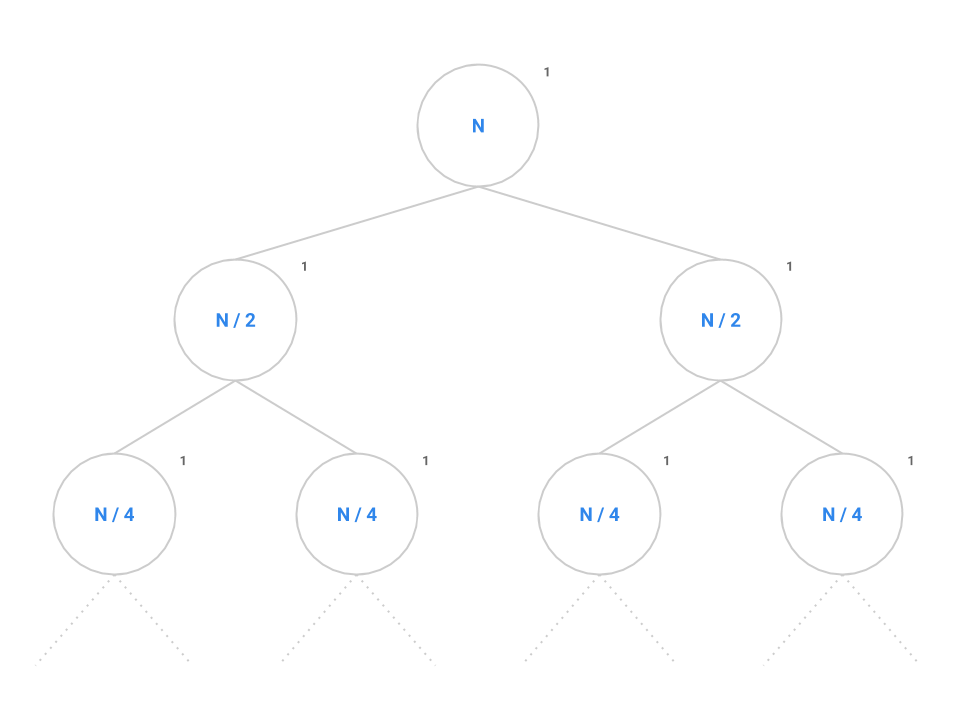
\includegraphics[scale=0.42]{images/02-bs-tree.png}
    \end{center}

    In each recursion step(level), we use 1 comparison(compare 
    $mid$ and $x$), then call recursion on a half 
    of the original array. From the image above, 
    we can easily notice there are total 
    $1+1+\cdots+1=1+\log_2 n$ comparisons.

    \newpage
    \section{Example: Towers of Hanoi}

    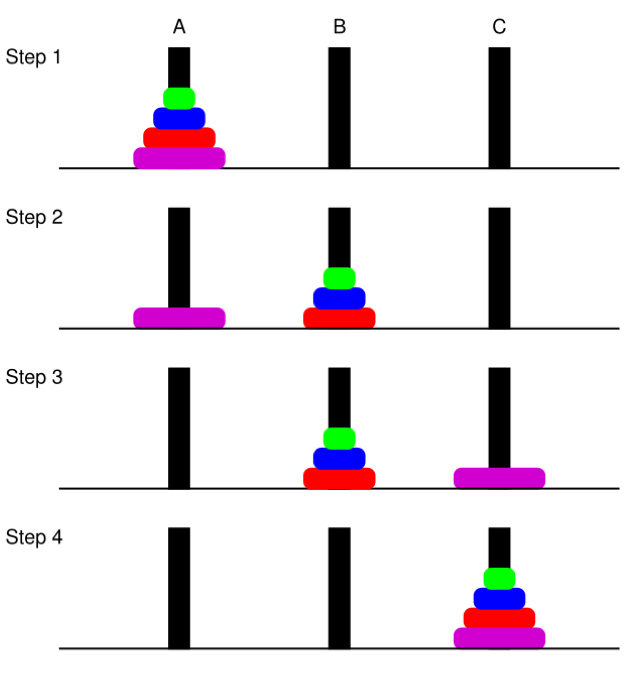
\includegraphics[scale=0.28]{images/02-hanoi.jpeg}
    
    In this example, we want to design an algorithm to 
    move all $n$ discs from peg $A$(start) to peg $C$(end), with the 
    constraints: (1) move one disc at a time, and 
    (2) cannot put larger disc on a smaller one.
    We are given another peg $B$(helper) where we can 
    temporary storage our discs.

    We still use the idea of {\bf Divide \& Conquer},
    consider how we can turn a problem of $n$ discs 
    into a problem of $n-1$? One possible solution is that,
    we can call recursion on upper $n-1$ discs, i.e., 
    move upper $n-1$ discs to peg $B$(helper peg), then move the remaining
    (the biggest) disc to peg $C$(end peg), and finally 
    move the $n-1$ discs from peg $B$(helper) to peg $C$(end).
    The following pseudocode shows this idea.

    \begin{algorithm}[H]
        \setstretch{1.1}
        \caption{MoveTower($n$, $start$, $helper$, $end$)}
        \KwIn{$n$: num of discs}
        \eIf{$n=1$}{
            move the only disc from $start$ peg to $end$ peg

            return
        }{
            {\tcp {move first $n-1$ from $start$ peg to $helper$ peg}}
            {\tcp {so this time ``helper'' peg will be the old $end$ peg}}
            {\bf MoveTower($n-1$, $start$, $end$, $helper$)}

            move the only disc from $start$ peg to $end$ peg

            {\tcp {finally move first $n-1$ from $helper$ peg to $end$ peg}}
            {\tcp {this time ``helper'' peg will be the old $start$ peg}}
            {\bf MoveTower($n-1$, $helper$, $start$, $end$)}
        }
    \end{algorithm}

    Now we would like to analyze the time complexity of this algorithm,
    in other words, how many {\bf steps} are needed.
    Let $T(n)$ be the num of steps for $n$ discs, each time, 
    we first move $n-1$ disks from $start$ to $helper$, 
    costs $T(n-1)$ steps; then we move the biggest disk to $end$ peg,
    costs only 1 step; finally we move $n-1$ disks from $helper$
    to $end$, again costs $T(n-1)$ steps. To sum up:
    $$T(n)=2T(n-1)+1$$ when $n>1$, and $T(1)=1$.

    Now we solve the recurrence by the {\bf expansion method}:
    \begin{align*}
        T(n) &= 2T(n-1) + 1\\
             &= 2[2T(n-2)+1] + 1\\
             &= 4T(n-2)+3\\
             &= 4[2T(n-3)+1] + 3 \\
             &= 8T(n-3) + 7\\
             &= \cdots \\
             &= 2^i T(n-i) + (2^i-1)\\
             &= 2^{n-1} T(1) + (2^{n-1}-1)\\
             &= 2^n-1
    \end{align*}

    Or, with the recursion tree method:
    \begin{center}
        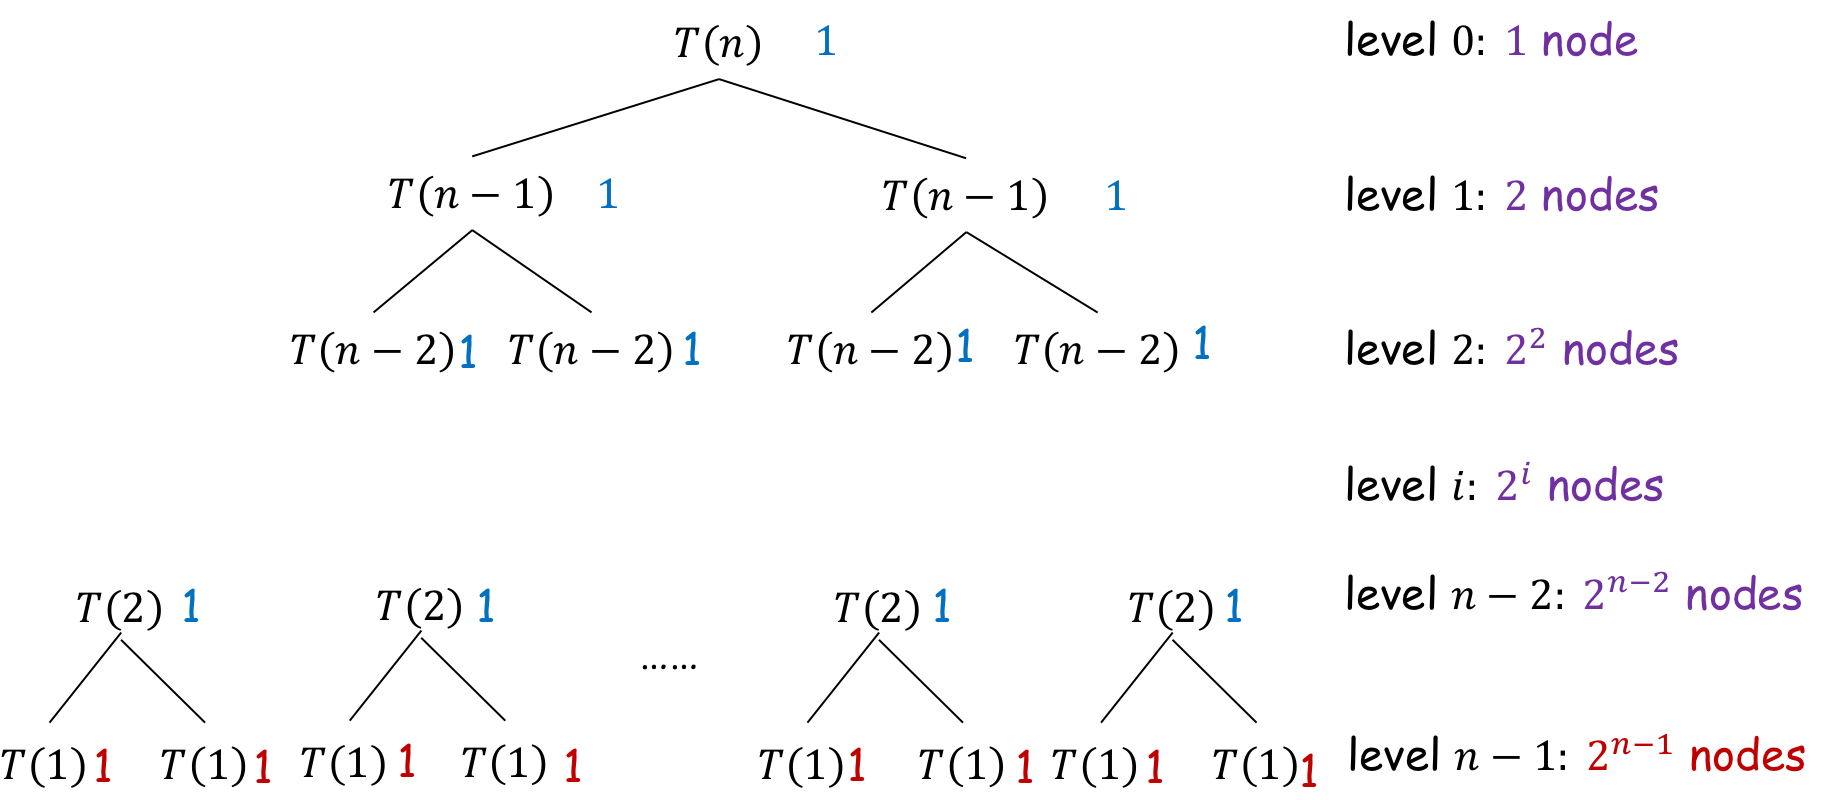
\includegraphics[scale=0.2]{images/02-hanoi-tree.jpeg}
    \end{center}
    
    There are, altogether, $1+2+2^2+2^3+\cdots + 2^{n-2}+2^{n-1}
    =2^n-1$ nodes, and we are doing one work(step) each node,
    then the time complexity is again, $2^n-1$.

    \newpage
    \section{Merge Sort}

    Now we again back to sorting, and we would like to introduce 
    a new algorithm or sorting: Merge Sort.
    This is a typical example of divide \& conquer, and 
    its process is like: (1) we first divide array into two halves,
    (2) then we recursively sort each half, (which means we 
    continuously divide it into halves, and then halves...)
    (3) finally {\bf merge} two halves to get a whole.

    The {\bf merge} operation may confuse you most. Here 
    it means combine two {\bf sorted lists} into a 
    whole sorted list. For example, given two sorted lists:
    $A=[2, 5, 7]$ and $B=[3, 4, 6, 10, 12]$, then after {\bf merge}
    operation, we will get $result=[2, 3, 4, 5, 6, 7, 10, 12]$.
    Since these two lists are sorted, we can do this process
    in $O(n)$ time, where $n$ is the length of result 
    list.(how many numbers in total) The basic idea is: 
    we compare the first item of $A$ and $B$, put the smaller 
    one, say, $A[1]$, in the first position of result list, then 
    we move on to the next item of $A$, but compare it still with 
    the {\bf first} item of $B$(since the first item of $B$
    has not yet inserted into result list), 
    and again put the smaller one into result list, then 
    continue move on. An example may help you understand the process:

    \noindent (1) Compare first items: $A=[{\blue 2},5,7], B=[{\blue 3},4,6,10,12]$, 
    $2<3$, so $result=[2]$;\\
    (2) then compare 2nd in $A$ and 1st in $B$, $A=[2, {\blue 5},7], B=[{\blue 3},4,6,10,12]$, 
    $3<5$, so $result=[2, 3]$;\\
    (3) continue the process, similarly, $A=[2, {\blue 5},7], B=[3,{\blue 4},6,10,12]$, 
    $4<5$, so $result=[2, 3, 4]$;\\
    (4) $A=[2, {\blue 5},7], B=[3,4,{\blue 6},10,12]$, 
    $5<6$, so $result=[2, 3, 4, 5]$;\\
    (5) $A=[2, 5,{\blue 7}], B=[3,4,{\blue 6},10,12]$, 
    $6<7$, so $result=[2, 3, 4, 5, 6]$;\\
    (6) $A=[2, 5,{\blue 7}], B=[3,4,6,{\blue 10},12]$, 
    $7<10$, so $result=[2, 3, 4, 5, 6, 7]$;\\
    (7) Now, all items in $A$ have already been inserted into result 
    list so that no items can be compared with items in $B$.
    Then we simply add remaining items in $B$ to result list,
    this will, obviously, ensure a sorted result list.(you may think of why)
    Hence $result=[2,3,4,5,6,7,{\blue 10,12}]$

    The pseudocode below shows the process:
    (below, append $\infty$ at the end of two lists can 
    free us from considering the situation that one list is 
    empty, like (7) above. Though different implementation, 
    the idea is entirely the same)
    
    \newpage
    \begin{algorithm}[H]
        \setstretch{1.1}
        \caption{Merge($A$, $left$, $mid$, $right$)}
        \tcp{merge two sorted list: $A[left\cdots mid]$ and $A[mid+1\cdots right]$}
        $L\lar A[left\cdots mid],\ R\lar A[mid+1\cdots right]$

        append $\infty$ at the end of $L$ and $R$ \qquad \tcp{see explanation above}

        $i\lar 1,\ j\lar 1$\qquad  \tcp{two pointers point at items in $L$ and $R$}

        \For{$k\lar left$ {\rm to} $right$} {
            \tcp{always choose the smaller one to insert, and move on}
            \eIf{$L[i] \le R[j]$}{
                $A[k]\lar L[i]$

                $i\lar i + 1$
            }{
                $A[k] \lar R[j]$

                $j\lar j + 1$
            }
        }
    \end{algorithm}

    After learning how {\bf Merge} works, you now, hopefully,
    are able to understand how Merge Sort works, with the image below:

    \begin{center}
        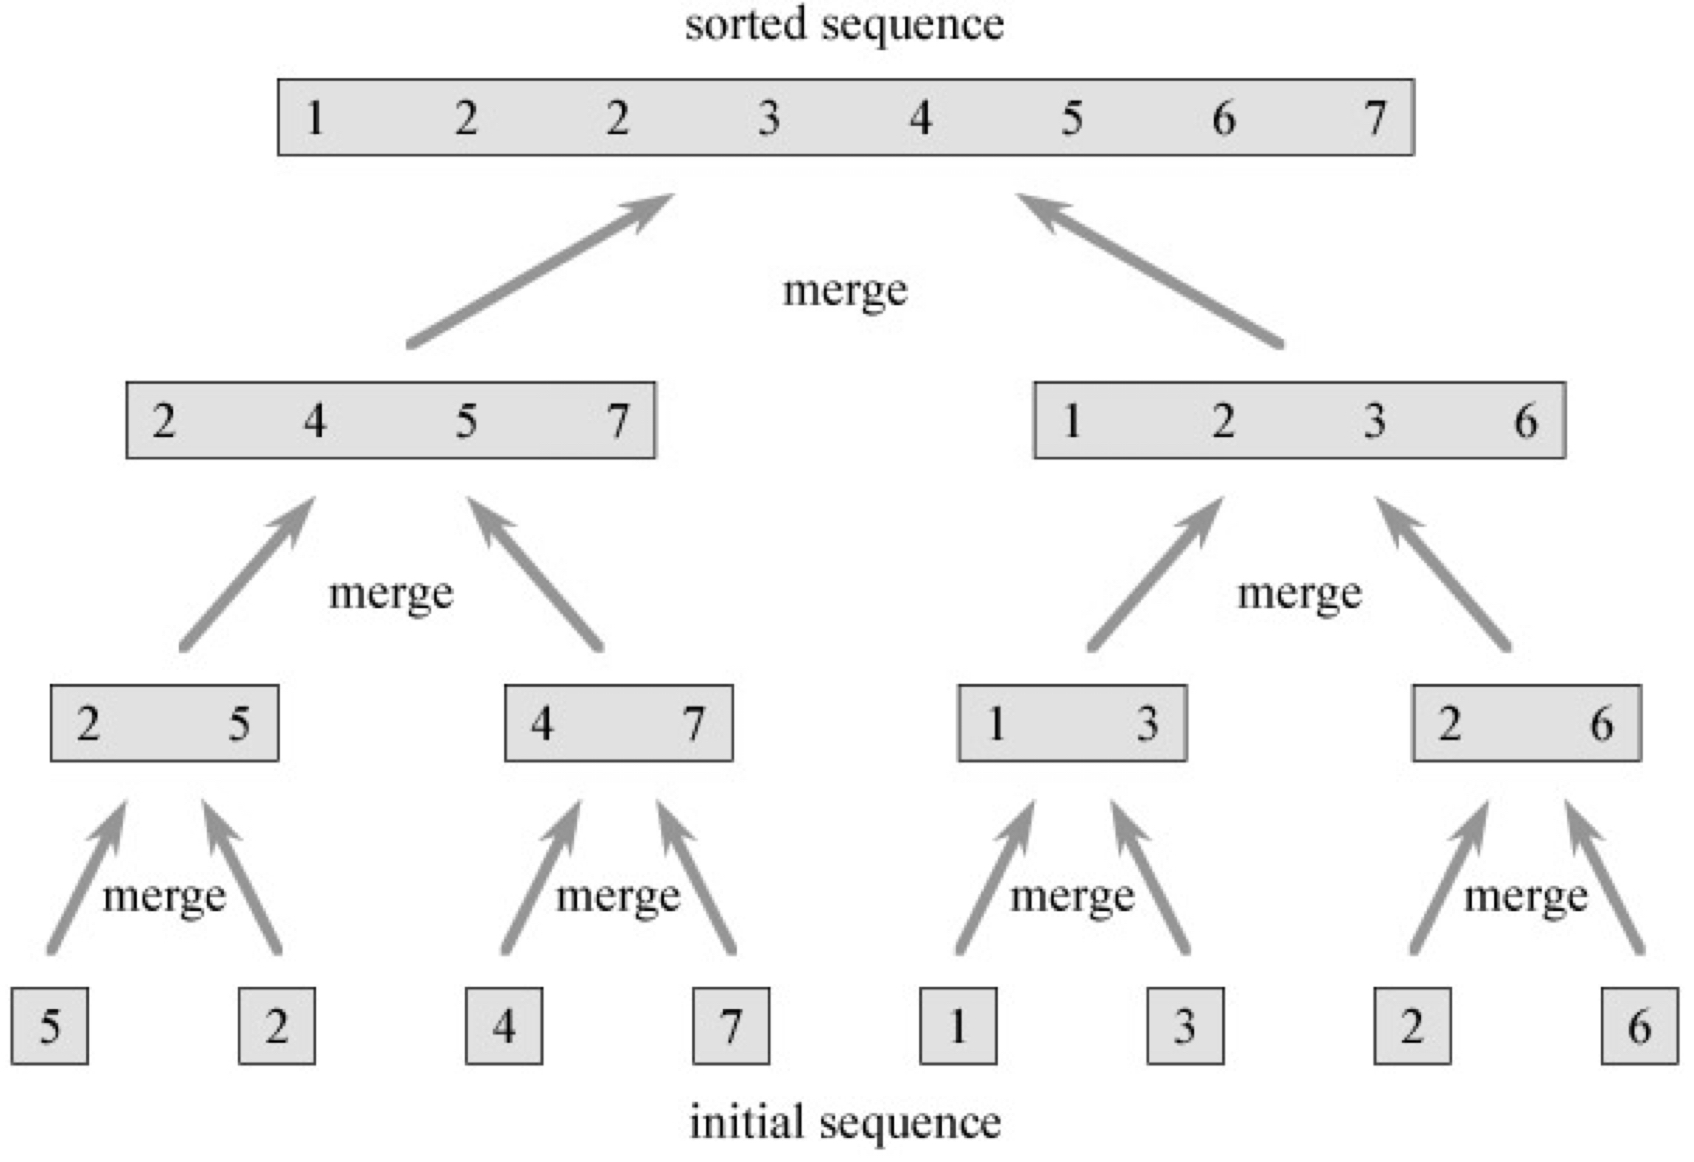
\includegraphics[scale=0.17]{images/02-mergeSort.jpeg}
    \end{center}
    
    We break down array recursively, until one element left,
    and then merge from bottom to up.
    The complete pseudocode for Merge Sort is given below:

    \newpage
    \begin{algorithm}[H]
        \setstretch{1.1}
        \caption{MergeSort($A$, $left$, $right$)}
        \If{$left=right$}{return}
        $mid\lar \lfloor (left + right) / 2 \rfloor$

        \tcp{recursively divide array into two halves}

        {\bf MergeSort($A$, $left$, $mid$)}

        {\bf MergeSort($A$, $mid+1$, $right$)}

        \tcp{then merge from bottom to up}

        {\bf Merge($A$, $left$, $mid$, $right$)}
    \end{algorithm}

    Firstly call {\bf MergeSort($A$, 1, $n$)} to sort array $A$.
    
    As usual, we are interested in the running time of Merge Sort 
    algorithm. Let $T(n)$ be the running time on an array of size $n$,
    it's not hard to find 
    $T(n)\le T(\lfloor n/2 \rfloor) + T(\lceil n/2 \rceil)+O(n)$,
    when $n>1$ and $T(1)=O(1)$.

    Here we are actually able to simplify the equation. Firstly 
    we can replace $\le $ with $=$, since we are interested
    in big-$O$ upper bound of $T(n)$; and with the same 
    reason, we can replace $O(n)$ with $n$, $O(1)$ with 1;
    finally, we can assume $n$ is a power of 2 for the sake of 
    simplicity but doesn't change the result at all, as 
    $T(n)\le T(n')\le T(2n)=O(T(n))$ where $n'$ is the 
    smallest power of 2 such that $n'\ge n$.

    Now we want to solve: 
    $T(n)=2T(n/2)+n$ for $n>1$, and $T(1)=1$.
    \begin{align*}
        T(n) &= 2\left(\frac{n}{2}\right)+n\\
             &= 2\left[ 2T\left(\frac{n}{4}\right) +\frac{n}{2}\right] + n
              = 2^2\cdot T\left(\frac{n}{2^2}\right) +2n\\
             &= 2^2\cdot \left[ 2T\left(\frac{n}{2^3}\right) +\frac{n}{2^2}\right] + 2n
              = 2^3\cdot T\left(\frac{n}{2^3}\right) +3n\\
             &= \cdots\\
             &= 2^{k}\cdot T\left(\frac{n}{2^k}\right) +kn
    \end{align*}
    We know the process ends with $\dfrac{n}{2^k}=1$ i.e. $k=\log_2 n$, thus
    \begin{align*}
        T(n) &= 2^{\log_2 n}T\left(\frac{n}{2^{\log_2 n}}\right)+n\cdot \log_2 n\\
             &= n\log_2 n+n
    \end{align*}
    In summary, merge sort runs in $O(n\log n)$ time.
    It is also worth pointing out that merge sort {\bf always}
    runs in $O(n\log n)$ time, which means best case is the same 
    as worst case, as you may think of it, 
    the complexity of merge sort {\it does not depend on inputs},
    it always break array down and then merge up.

    \newpage
    \section{Inversion Numbers}

    Given an array $A[1\cdots n]$, we say two elements $A[i]$ and $A[j]$
    are {\bf inverted} if $i<j$ but $A[i]>A[j]$, i.e., $A[i]$ appears
    before $A[j]$ but is larger than $A[j]$. The number of inverted pairs
    is called the {\bf inversion number} of array $A$. 
    Actually this is a useful measure, it provides us with an intuitive
    idea about how ``sorted'' an array is, larger inversion number implies
    a more unsorted array.

    What may surprise you is that inversion number has a close relation
    to insertion sort, and more concretely, {\bf the number of swaps
    used by insertion sort is equals to inversion number.}
    We can prove it by induction:
    
    \begin{proof}
        Assuming the array has size $n$. Basic case
        $n=2$ obviously holds.

        Inductive step: assume correct for an array of size $n-1$, i.e.,
        the total number of swaps performed while insertion sorting
        $A[1\cdots n-1]$ is equals to the inversion number of $A[1\cdots n-1]$.

        Let $x=A[n]$. Now, the remaining work by insertion sort is that we swap 
        $x$ with all items $A[j]$ such that $j<n$ and $A[j]>x$, 
        notice that the number of those items is the same of inversions in which
        {\bf $x$ participates}. Therefore, adding these new inversions gives
        the full inversion number of $A[1\cdots n]$.
    \end{proof}

    Now we will consider how to compute the inversion number of a given 
    array with size $n$. One possible method is we check all $(i,j)$
    pairs of given array, this requires ${n\choose 2}=\Theta(n^2)$
    running time. Another method uses the relation we proved above,
    running insertion sort and count the number of swaps we perform,
    but this also requires $\Theta(n^2)$ time since insertion sort 
    requires $\Theta(n^2)$. How can we improve that? 
    Come back to topic: divide and conquer!

    Similar to previous problems, we divide array into two halves, 
    and recursively count inversions in each half, but notice:
    we are missing something: we still need to count inversions
    where $a_i$ and $a_j$ are in different halves! We need 
    to return the sum of those three quantities finally.

    So the main problems is that, how we count the third quantity?
    Consider below situation, the two halves of array are:
    $[1,5,4,8,10,2]$ and $[6,9,12,11,3,7]$, how would you do that?
    You may count by hand, and knowing there are $5-3, 4-3, 8-6, \cdots$
    and in total 9 inversions with one item in 1st array and another in 
    2nd. But, it's really time consuming and totally a mess! We have 
    no efficient algorithm to do this but to count one by one.

    Fortunately, things will become much better if those two arrays are 
    {\it sorted}. For example, $A=[3,7,10,14,18,19]$ and 
    $B=[2,11,16,17,23,25]$. How will we do then? We can 
    scan progressively through both lists, and for each item 
    in $B$, we only need to find the smallest $A$ item 
    larger than it. In the lists above, for example, $A[1]=3$
    is larger than $B[1]=2$, so all items in $A$ form an inversion pair 
    with $B[1]$; then we move to $B[2]=11$, we try to find the smallest 
    item in $A$ larger than 11, so we move the pointer in $A$, 
    $A[2]=7<11, A[3]=10<11$, until $A[4]=14>11$, so 
    each item in $A[4]\cdots A[6]$ can form an inversion pair with $B[2]$.
    If we continue the process, we will finally get the inversion 
    number formed between $A$ and $B$, in $O(n)$ time. (Why is $O(n)$?
    Since we only iterate each item once during the whole process.
    You may find it quite similar to Merge operation in Merge Sort)

    \begin{algorithm}[H]
        \setstretch{1}
        \caption{Count($A$, $l$, $mid$, $r$)}
        \tcp{
            $l$ means left, while $r$ means right.
        }

        \tcp{notice here, $L[1\cdots (mid-l+1)]$ is corresponding to 
        $A[l\cdots mid]$, the subscript changes, try not be confused later.
        $R$ also changes.}
        $L\lar A[l\cdots mid],\ R\lar A[mid+1\cdots r]$

        (here assume) $L, R$ already sorted

        $i\lar 1,\ j\lar 1$\qquad \tcp{two pointers for $L$ and $R$}

        $ans\lar 0$ \qquad \tcp{total inversion number}

        \tcp{let $i,j$ iterator over two arrays}
        \While{$i\le mid-l+1$ and $j\le r-mid$}{
            \tcp{looking for smallest $L$ item larger than $R$}
            \eIf{$L[i]\le R[j]$}{ 
                $i\lar i+1$
            }{
                \tcp{Found $L[i] > R[j]$!}

                \tcp{then $L[i]\cdots L[mid-l+1]$ each can form an inversion pair with $R[j]$,
                remind here $L$ subscript is diff from $A$, as stated above}

                \tcp{so inversion num for $R[j]$ is $mid-l+1-i+1=mid-l-i+2$}

                $inv\lar (mid-l-i+2)$

                $ans\lar ans+inv$

                $j\lar j+1$
            }
        }
        return $ans$
    \end{algorithm}

    And, the whole algorithm for counting the inversion number will be:

    \begin{algorithm}[H]
        \setstretch{1.1}
        \caption{Count-Inversion($A$, $l$, $r$)}
        \If{$l=r$}{
            return 0
        }
        $mid \lar \lfloor (l+r)/2 \rfloor$

        $c_1\lar$ Count-Inversion($A$, $l$, $mid$)

        $c_2\lar$ Count-Inversion($A$, $mid+1$, $r$)

        MergeSort($A$, $l$, $mid$) 

        MergeSort($A$, $mid+1$, $r$) 

        $c_3\lar$ Count($A$, $l$, $mid$, $r$)

        return $c_1+c_2+c_3$
    \end{algorithm}

    First call: Count-Inversion($A$, 1, $n$).

    So far, you may think this is an excellent algorithm since we 
    only use $O(n)$ in each recursion step. However, it isn't! 
    Remember, we have assumed each half is already sorted, but in fact 
    they are random. If we firstly run some sort algorithm, say, 
    Merge Sort, and then do the counting above, the whole 
    running time will be:
    $$T(n)=2T(n/2)+\Theta (n\log n+n)=2T(n/2)+\Theta (n\log n)$$
    One can show $T(n)=\Theta(n\log^2 n)$.

    This is, to a certain degree, acceptable, compared to previous $\Theta(n^2)$,
    but we still want to improve that. 
    We can easily notice the main problem lies in sorting, which 
    uses $\Theta(n\log n)$ in each recursion step. How can we 
    reduce, or even avoid this process? 

    This is indeed hard to think about, but we can combine the sorting process 
    (more concretely, Merge sort)
    with the process which we count inversion pairs that form between the 
    two halves. In other words, previously we only do counting between 
    two halves, now we also perform Merge at the same time.
    What will this lead to? Consider from recursion bottom(1 item), 
    to top, each time we Merge the two halves, as what we did in 
    Merge Sort, and at the same time, count inversion pairs that cross 
    the two halves. And since we Merge from bottom to top, 
    the two halves will always be sorted.(this is exactly the same 
    Merge in Merge Sort)

    The paragraph above is still so abstract, at least for myself, 
    perhaps it's better to look at how the algorithm is implemented.\\

    \begin{algorithm}[H]
        \setstretch{1}
        \caption{Merge-and-Count($A$, $l$, $mid$, $r$)}

        \tcp{same as previous algorithm, subscripts for $L,R$ and $A$
        are different, remember this}

        $L\lar A[l\cdots mid],\ R\lar A[mid+1\cdots r]$

        append $\infty$ at the end of $L$ and $R$

        $i\lar 1,\ j\lar 1$ \qquad \tcp{two iteration pointers for $L$ and $R$}

        $count \lar 0$  \qquad \tcp{counter for inversion number}

        \For{$k\lar l$ to $r$}{
            \eIf{$L[i]\le R[j]$}{
                $A[k]\lar L[i]$

                $i\lar i+1$
            }{
                $A[k]\lar R[j]$

                $j\lar j+1$

                $count \lar count + (mid-l-i+2)$
            }
        }
        return $count$

    \end{algorithm}

    As you can find out above, apart from count inversion pairs 
    between $L$ and $R$, we merge them into a new array $A$,
    this is exactly what we did in merge sort, which maintains
    the ``sorted'' invariant. With the function above, 
    the complete algorithm for finding inversion number for an array is 
    displayed below.

    \begin{algorithm}
        \caption{Sort-and-Count($A$, $l$, $r$)}

        \If{$l=r$}{
            return 0
        }
        $mid\lar \lfloor (l+r)/2\rfloor$

        $c_1\lar $ Sort-and-Count($A$, $l$, $mid$)

        $c_2\lar $ Sort-and-Count($A$, $mid+1$, $r$)

        $c_3\lar $ Merge-and-Count($A$, $l$, $mid$, $r$)

        return $c_1+c_2+c_3$
    \end{algorithm}

    First call: Sort-and-Count($A$, 1, $n$)

    \newpage
    \section{The Maximum Subarray Problem}

    {\bf Problem:} Given an array of size $n$, the task is
    to find the largest possible sum of a contiguous subarray.
    For example, given $[3,2,1,-7,5,2,-1,3,-1]$, 
    subarray $[5,2,-1,3]$ has the largest sum among all subarrays,
    we need to output $5+2+(-1)+3=9$.

    We will provide a lot of algorithms to solve this problem.

    \subsection{brute force algorithm}

    The simplest idea is, for each pair $(i,j)$, we calculate
    $A[i]+A[i+1]+\cdots+A[j]$, and record maximum value 
    we have seen along the process.

    \begin{algorithm}
        \caption{Max-Subarray-Brute-Force($A$)}
        $maxSum \lar A[1]$ \qquad \tcp{can also use -inf to initialize}

        \For{$i\lar 1$ to $n$}{
            \For{$j\lar i$ to $n$}{
                \tcp{calculate $A[i]+\cdots+A[j]$}

                $sum\lar 0$

                \For{$k\lar i$ to $j$}{
                    $sum \lar sum + A[k]$
                }
                \tcp{if current $sum$ is larger, update $maxSum$}
                \If{$sum > maxSum$}{
                    $maxSum \lar sum$
                }
            }
        }
        return $maxSum$
    \end{algorithm}

    This is a very simple algorithm, but requires $\Theta(n^3)$ running time.

    \subsection{prefix sum}

    In brute force algorithm, we notice that each time when we 
    calculate $A[i]+A[i+1]+\cdots+A[j]$, we need to iterate through 
    these items, and add them together, which requires a lot of 
    redundant work. The {\bf prefix sum}, say $S[i]$, is defined 
    as $\sum_{j=1}^{i} A[i]$, i.e., the sum of all items before(and include)
    $A[i]$. If we have a table of all $S[i]$ values, we can now rewrite 
    $\sum_{k=i}^{j} A[k]=S[j]-S[i-1]$. See? That's a $\Theta(1)$ job!

    \vspace{0.2in}
    \begin{algorithm}
        \setstretch{1.5}
        \caption{Get-Prefix-Sum($A$)}
        \tcp{$S[]$ records the prefix sum of array $A$}
        $S[0]=0$

        \For{$i=1$ to $n$}{
            $S[i]\lar S[i-1]+A[i]$
        }
        return $S$
    \end{algorithm}

    \begin{algorithm}[H]
        \setstretch{1}
        \caption{Max-Subarray-Prefix-Sum($A$)}
        $maxSum \lar A[1]$ 

        $S\lar$ Get-Prefix-Sum($A$) \qquad \tcp{get prefix sum}

        \For{$i\lar 1$ to $n$}{
            \For{$j\lar i$ to $n$}{
                $sum\lar S[j]-S[i-1]$ \qquad \tcp{calculate $A[i]+\cdots+A[j]$}

                \If{$sum > maxSum$}{
                    $maxSum \lar sum$
                }
            }
        }
        return $maxSum$
    \end{algorithm}

    This reduces the running time of our algorithm to $\Theta(n^2)$.
    (Calculating prefix sum only requires $\Theta(n)$, 
    so overall $\Theta(n^2+n)=\Theta(n^2)$)

    \subsection{divide and conquer}

    Again, we return to our topic, and again, we try to cut 
    the array into two halves. Similar to {\bf Inversion Number}
    example, we classified all subarrays into three cases:
    \begin{enumerate}
        \item entirely in the first half
        \item entirely in the second half
        \item crosses the cut
    \end{enumerate}
    I think it will not surprise you that the third situation is 
    the most difficult one, while the first two cases, can still 
    be found recursively.

    \newpage
    \begin{algorithm}[H]
        \setstretch{1}
        \caption{Max-Subarray-Divide-Conquer($A$, $l$, $r$)}

        \If{$l=r$}{return $A[l]$}

        $mid\lar \lfloor (l+r)/2 \rfloor$

        $max_1\lar $ Max-Subarray-Divide-Conquer($A$, $l$, $mid$)

        $max_2\lar $ Max-Subarray-Divide-Conquer($A$, $mid+1$, $r$)

        $max_3\lar $ Max Subarray that crosses the cut

        return $\max \{ max_1, max_2, max_3 \}$
    \end{algorithm}

    So how can we efficiently calculate $max_3$? Firstly, consider 
    what do we mean by ``crosses the cut''? That should be, 
    the subarray will {\it at least include both $A[mid]$ and $A[mid+1]$}
    in order to ``cross''. Hence these kind of subarray can always be 
    divided into two parts: $A[i\cdots mid]$ and $A[mid+1\cdots j]$
    for some $i$ and $j$. So in order to find max $A[i]+\cdots +A[j]$,
    we just find max $A[i]+\cdots +A[mid]$, and $A[mid+1]+\cdots +A[j]$,
    and finally add them together, this will definitely give us 
    the max value.

    Alright, so how can we find $i$?(and can use exactly the same 
    method to find $j$)
    It should be the index that maximize $A[i]+\cdots +A[mid]$.
    This is much easier since one end, say, $mid$, is fixed.
    We initialize $maxSum$ to $-\infty$, then scan from $mid$ towards left,
    each step we add an item to temporary $sum$, and update 
    $maxSum$ if $sum$ is larger. When we reach $l$(left end), 
    we will have already iterated all possible indices $i$ and 
    stored the max sum in $maxSum$.
    
    \begin{algorithm}[H]
        \setstretch{1}
        \caption{Max-Subarray-Divide-Conquer($A$, $l$, $r$)}

        \If{$l=r$}{return $A[l]$}

        $mid\lar \lfloor (l+r)/2 \rfloor$

        $max_1\lar $ Max-Subarray-Divide-Conquer($A$, $l$, $mid$)

        $max_2\lar $ Max-Subarray-Divide-Conquer($A$, $mid+1$, $r$)

        \tcp{now let's count $max_3$}

        $L_m\lar -\infty,\ R_m\lar -\infty$

        $sum\lar 0$

        \For{$i=mid$ down to $l$}{
            $sum\lar sum + A[i]$

            \If{$sum > L_m$}{$L_m\lar sum$}
        }

        $sum\lar 0$

        \For{$i=mid+1$ to $r$}{
            $sum\lar sum + A[i]$

            \If{$sum > R_m$}{$R_m\lar sum$}
        }

        return $\max \{ max_1, max_2, L_m+R_m \}$
    \end{algorithm}

    First call {\bf Max-Subarray-Divide-Conquer($A$, 1, $n$)}.

    It's not difficult to find out the process of finding $max_3$
    requires $O(n)$ time, since we just scan throughout the array.
    If let $T(n)$ be the running time of whole algorithm, 
    we will get:
    $$T(n)=2T(n/2)+O(n)$$
    This gives $T(n)=O(n\log n)$.

    \subsection{linear time?}

    Review the idea of calculating $max_3$ above, we said that 
    finding max $A[i]+\cdots +A[mid]$ is much easier since $mid$
    is a fixed ending point. This gives us an inspiration:
    for a {\it fixed} $j$, finding largest $A[i]+\cdots +A[j]=
    S[j]-S[i-1]$, is the same as finding the smallest $S[i-1]$
    .(Recall that $S[]$ is the prefix sum)
    If we can find the smallest $S[i-1]$ for each $j$,
    we will able to find the max subarray.(here $i-1$ must 
    be strictly smaller than $j$, otherwise the subarray is null)

    The process of finding smallest $S[i-1]$ can be easily done 
    during the iteration through array. More concretely, 
    we only need to update $minS = \min\{minS, A[i]\}$ at each step.
    Below shows the entire algorithm.
    
    \begin{algorithm}
        \caption{Max-Subarray-Linear($A$)}
        \tcp{Here we initialize $minS$ to 0 because {\it at least}
        we can do $S[j]-S[0]$ to ensure the sum is {\it at least}
        not smaller than $S[j]$}
        $maxSum \lar -\infty,\ minS\lar 0$

        \tcp{for each $j$, find $minS$, and then find $S[j]-minS$}
        \For{$j\lar 1$ to $n$}{
            \tcp{update overall answer}
            \If{$S[j]-minS>maxSum$}{
                $maxSum\lar S[j]-minS$
            }
            \tcp{update $minS$ so far}
            \If{$S[j] < minS$}{
                $minS\lar S[j]$
            }
        }
        return $maxSum$
    \end{algorithm}

    This algorithm can also be written without calculating prefix sum 
    before, since each time we only use $S[j]$, we only need one
    variable to record $S[j]$ and accumulate it each time.

    \newpage
    \begin{algorithm}
        \setstretch{1}
        \caption{Max-Subarray-Linear2($A$)}
        \tcp{$S$ will be all prefix sum so far, i.e., $A[1]+\cdots+A[j]$}
        $maxSum \lar -\infty,\ minS\lar 0,\ S\lar 0$

        \For{$j\lar 1$ to $n$}{
            $S\lar S+A[j]$ \qquad \tcp{calculate prefix sum so far}
            \If{$S-minS>maxSum$}{
                $maxSum\lar S-minS$
            }
            \tcp{update $minS$ so far}
            \If{$S < minS$}{
                $minS\lar S[j]$
            }
        }
        return $maxSum$
    \end{algorithm}

    As you can see, this algorithm only requires linear $\Theta(n)$ time.
    It is indeed a difficult progress that we optimize the algorithm 
    from $\Theta(n^3)$ down to $\Theta(n)$, with lots of new ideas 
    come out. We say this is ``More art than science''.

    \subsection{dynamic programming}

    By using {\bf dynamic programming} ideas, which we will formally 
    introduce later, we can also design quite efficient algorithms,
    but efficient always requires more thinking.
    Here we just give you a first taste on DP.

    We define $d[i]$ be the max sum of subarray that {\it 
    ends with $A[i]$}. Here we must contain $A[i]$ in 
    $d[i]$, otherwise, we cannot get $d[i+1]$ from $d[i]$,
    because it will break the ``consecutive'' subarray requirement.
    But if you ask me why we define in such a way, I cannot 
    explain it, and that is the ``art of dynamic programming'' :)

    So when we calculating $d[i]$, we only need to check $d[i-1]$
    and $A[i]$, this is the basic idea of dynamic programming, 
    that is, get value from previous values.
    And if $d[i-1]\le 0$, which means $d[i-1]+A[i]$ is not larger than 
    $A[i]$ itself! So why should we include $d[i-1]$ then, 
    we just let $d[i]=A[i]$, this will be the max sum with 
    $A[i]$ included.
    On the contrary, if $d[i-1]>0$, then we should let 
    $d[i]=d[i-1]+A[i]$, since include $d[i-1]$ makes the sum 
    larger, and that is exactly what we want.

    \newpage
    \begin{algorithm}[H]
        \setstretch{1}
        \caption{Max-Subarray-DP($A$)}
        $d[0]\lar 0$ \qquad \tcp{max sum of subarrays end with no item is 0}

        $maxSum\lar A[1]$\qquad \tcp{used to record max sum so far, notice here cannot initialize to 0}
        \For{$i=1$ to $n$}{
            \eIf{$d[i-1]\le 0$}{
                $d[i]\lar A[i]$
            }{
                $d[i]\lar d[i-1]+A[i]$
            }
            \If{$d[i]>maxSum$}{$maxSum=d[i]$}
        }
        return $maxSum$
    \end{algorithm}

    This is also a $\Theta(n)$ algorithm, and as usual, it is not easy 
    to think. But, we can still reduce the space it takes, i.e., 
    space complexity. Notice here we use an array $d[i]$ to record 
    the max sum of subarrays end with $A[i]$, but each time, 
    say, when we calculate $d[i]$, we only use the previous one,
    say, $d[i-1]$. So it is no need that we use an array to track this:
    we only need a variable to record the previous $d$ value,
    that's enough! So we can slightly modify the algorithm as below:

    \begin{algorithm}[H]
        \setstretch{1}
        \caption{Max-Subarray-DP2($A$)}
        $previousD\lar 0$ 

        $maxSum\lar A[1]$

        \For{$i=1$ to $n$}{
            \eIf{$previousD\le 0$}{
                $previousD\lar A[i]$
            }{
                $previousD\lar previousD+A[i]$
            }
            \If{$previousD>maxSum$}{$maxSum=previousD$}
        }
        return $maxSum$
    \end{algorithm}

    \newpage
    \section{The Master Theorem}

    \subsection{Theorem and its proof}

    {\bf The Master Theorem:} Let $a\ge 1, b>1, c\ge 0$
    be constants, if $T(n)=aT(n/b)+n^d$, then:
    \begin{align*}
        \setstretch{0.7}
        T(n)=\left\{ \begin{array}{ll}
            O(n^d), & \text{if } d>\log_b{a}\\
            O(n^d\log n), & \text{if } d = \log_b{a}\\
            O(n^{\log_b{a}}), & \text{if } d < \log_b{a}\\
        \end{array}\right.
    \end{align*}

    There is one kind of proof given in lecture slide, 
    using expansion method. But personally, I like the method below.

    \begin{proof}
    Consider $T(n)=a\cdot T\left(\dfrac{n}{b}\right)+c\cdot n^{d}$,
    for the 0th layer of recursion(since we haven't begun recursion),
    running time is $c\cdot n^{d}$;
    for the 1st layer, there are $a$ branches, and each
    branch has running time $c\cdot \left(\dfrac{n}{b}\right)^d$, 
    in total $c\cdot \left(\dfrac{a}{b^d}\right)\cdot n^d$;
    for the 2nd layer, each branch in 1st layer has $a$ branches,
    so there are $a^2$ branches now, with each requires 
    $c\cdot \left(\dfrac{n}{b^2}\right)^d$, and 
    $c\cdot \left(\dfrac{a}{b^d}\right)^2\cdot n^d$ in total.
    We can easily find the pattern: 
    the running time of $k$-th layer is 
    $c\cdot \left(\dfrac{a}{b^d}\right)^k\cdot n^d$.

    Add all of them together, we get 
    $$T(n)=c\cdot n^d\cdot \left[ 1+ \left(\dfrac{a}{b^d}\right)+\cdots + \left(\dfrac{a}{b^d}\right)^k\right]$$

    Recall the sum of geometric sequence:
    \begin{align*}
        \setstretch{0.7}
        1+p+p^2+\cdots +p^k=\left\{
        \begin{array}{ll}
            k+1, & \text{if } p=1\\
            \dfrac{p^{k+1}-1}{p-1}, & \text{if } p\ne 1
        \end{array}\right.
    \end{align*}

    Condition 1: when $a=b^d$, ratio is 1, so $T(n)=O(n^d\log n)$.

    Condition 2: when $a<b^d$, the sequence is decreasing, 
    so the sum is determined by the first item(you can also 
    infer from the equation of sum above), then $T(n)=O(n^d)$.

    Condition 3: when $a>b^d$, the sequence is increasing, 
    the sum is determined by the last item, this gives 
    $T(n)=n^{d}\left(\dfrac{a}{b^{d}}\right)^{\log _{b} n}=
    n^{d}\left(\dfrac{a^{\log _{b} n}}{\left(b^{\log _{b} n}\right)^{d}}\right)=
    a^{\log _{b} n}=
    \left(n^{\log_n{a}}\right)^{\log_b{n}}=
    n^{\left(\frac{\ln a}{\ln n}\cdot \frac{\ln n}{\ln b}\right)}=
    n^{\log _{b} a}$.
    \end{proof}

    \newpage
    \subsection{equalities, inequalities and more}

    {\Large\color{red} to be added. (2021/09/05)}

    \newpage
    \section{Integer Multiplication}

    You may first think of using primary school method: 
    i.e., ``long multiplication'', and this requires $\Theta(n^2)$
    time. We will show that we can do better than this, but 
    the ideas are quite difficult to think of, and actually 
    people used quite a long time to invent the algorithms.

    \subsection{divide and conquer: first attempt}

    For example, we would like to calculate $3711\times 4021$,
    we can divide each number into two parts: {\bf high} part 
    and {\bf low} part, say, $x_h=37, y_h=40$, and $x_l=11, y_l=21$.
    Then, $x\times y=x_h\times y_h\cdot 10^n+(x_l\times y_h+x_h\times 
    y_l)\cdot 10^{n/2}+x_l\times y_l$, where $n$ is the length of 
    two numbers. One thing worths mentioning is that we can always 
    take $n$ as a perfect square of 2, and if it is not, we just 
    put some 0s in front of the number.
    So now, there are four multiplications and we can use recursion 
    to calculate each of them. And for multiplying power of 10, 
    we can just think of it as adding some 0s after the number, so 
    this takes $O(n)$ time.

    \begin{algorithm}
        \caption{multiply-DC($A$, $B$)}
        \tcp{$A[1\cdots n]$ and $B[1\cdots n]$ are two arrays storing 
        string of base 10. $A[1], B[1]$ are least siginificant bits.(LSB)}

        $n\lar $ size of $A$ and $B$

        \If{$n=1$}{return $A[1]\cdot B[1]$}

        $mid\lar \lfloor n/2 \rfloor$

        $M_1\lar $multiply-DC($A[mid+1\cdots n]$, $B[mid+1\cdots n]$)
        \qquad \tcp{$x_h\times y_h$}

        $M_2\lar $multiply-DC($A[1\cdots mid]$, $B[mid+1\cdots n]$)
        \qquad \tcp{$x_l\times y_h$}

        $M_3\lar $multiply-DC($A[mid+1\cdots n]$, $B[1\cdots mid]$)
        \qquad \tcp{$x_h\times y_l$}

        $M_4\lar $multiply-DC($A[1\cdots mid]$, $B[1\cdots mid]$)
        \qquad \tcp{$x_l\times y_l$}

        \tcp{Below we can put numbers in array directly, or 
        append 0 at the end and add them together.
        Assume $res[]$ is filled with 0 at the beginning.}

        $res[1\cdots n]\lar M_4$

        $res[mid+1\cdots ]\lar res[mid+1\cdots] + M_2+M_3$

        $res[n+1\cdots]\lar res[n+1\cdots]+M_1$

        return $res$
    \end{algorithm}

    This will require a running time as $T(n)=4T(n/2)+O(n)$, 
    hence $T(n)=O(n^2)$, which doesn't improve our algorithm 
    at all. One may think of using binary representation(base 2)
    instead of decimal, but this doesn't help either, 
    though multiply by power of 2 can be done in $O(1)$ time, 
    with the help of left shift($<<$), write the result into 
    the array still takes $O(n)$, regardless of the time 
    converting an integer of base 10 into base 2. 
    So basically, we need to reduce the time we call recursion 
    to reduce the running time.

    \subsection{Karatsuba's method}

    As shown above, we need to calculating 4 multiplications,
    which makes us to call 4 recursions. Trying to improve that, 
    Karatsuba noticed that we only need $x_h\times y_l+x_l\times y_h$(the sum),
    instead of calculating each of the multiplication result.
    He suggested we only need to calculate 3 times, and they are:
    $M_1=x_h\times y_h, M_2=x_l\times y_l, M_3=(x_h+x_l)\times 
    (y_h+y_l)$, then we can get $x_h\times y_l+x_l\times y_h$ 
    by doing $M_3-M_1-M_2$. This successfully reduce the 
    running time of multiplication algorithm, with only 3 
    recursion calls:
    $T(n)=3T(n/2)+O(n)$, gives $T(n)=n^{\log_2 3}\approx n^{1.585}$.

    \begin{algorithm}
        \caption{Karatsuba($A$, $B$)}
        \tcp{$A[1\cdots n]$ and $B[1\cdots n]$ are two arrays storing 
        string of base 10. $A[1], B[1]$ are LSB.}

        $n\lar $ size of $A$ and $B$

        \If{$n=1$}{return $A[1]\cdot B[1]$}

        $mid\lar \lfloor n/2 \rfloor$

        $M_1\lar $Karatsuba($A[mid+1\cdots n]$, $B[mid+1\cdots n]$)
        \qquad \tcp{$x_h\times y_h$}

        $M_2\lar $Karatsuba($A[1\cdots mid]$, $B[1\cdots mid]$)
        \qquad \tcp{$x_l\times y_l$}

        $A'\lar A[mid+1\cdots n]+A[1\cdots mid]$

        $B'\lar B[mid+1\cdots n]+B[1\cdots mid]$

        $M_3\lar $Karatsuba($A'$, $B'$)
        \qquad \tcp{$(x_h+x_l)\times (y_h+y_l)$}

        \tcp{Assume $res[]$ is filled with 0 at the beginning.}

        $res[1\cdots n]\lar M_2$

        $res[mid+1\cdots ]\lar res[mid+1\cdots] +M_3-M_1-M_2$

        $res[n+1\cdots]\lar res[n+1\cdots]+M_1$

        return $res$
    \end{algorithm}

    \subsection{So far...}

    Inspired by Karatsuba, people can improve his algorithm by 
    ``dividing each integer into 3 parts, and solve 5 multiplications'',
    or ``divide into $n$ parts, and solve $2n-1$ multiplications'' etc.
    Later on, in 1971, Strassen solved this problem in 
    $O(n\log n\log \log n)$, using {\bf Fast Fourier Transformation(FFT)}.
    In 2007, $O(n\log n\cdot 8^{\log ^* n})$ algorithm was found 
    and in 2019, finally, $O(n\log n)$ algorithm was found.

    However, Karatsuba's algorithm isn't always faster than 
    our primary school $O(n^2)$ method, since it has a larger 
    constant. In practice, people find that for integers with
    length less than 20, using our $O(n^2)$ method is better;
    while Karatsuba's algorithm is better for length $20\sim 2000$,
    FFT is better for $>2000$. And for your reference, Python 
    uses 70 as a critical value to judge whether to perform 
    primary school method or Karatsuba's method.

    \newpage
    \section{Matrix Multiplication}

    Given two $n\times n$ matrices $A, B$, how can we compute 
    $C=AB$?
    
    Since $c_{ij}=\sum_{k=1}^{n}a_{ik}b_{kj}$, 
    we can use three nested loops to calculate each items in $C$,
    in $\Theta(n^3)$ time. This is our brute force algorithm.

    \subsection{divide and conquer?}

    Much similar to integer multiplication, we try to divide 
    $A$ and $B$ into $\frac{1}{2}n\times \frac{1}{2}n$ matrices 
    and call recursion to multiply each part.
    \begin{align*}
        \setstretch{0.5}
        \left[ \begin{array}{cc}
            C_{11} & C_{12} \\
            C_{21} & C_{22}
        \end{array} \right]
        =
        \left[ \begin{array}{cc}
            A_{11} & A_{12} \\
            A_{21} & A_{22}
        \end{array} \right]
        \left[ \begin{array}{cc}
            B_{11} & B_{12} \\
            B_{21} & B_{22}
        \end{array} \right]
    \end{align*}
    and,
    \begin{align*}
        C_{11} &= (A_{11}\times B_{11}) + (A_{12}\times B_{21}) \qquad 
        C_{12} = (A_{11}\times B_{12}) + (A_{12}\times B_{22}) \\
        C_{21} &= (A_{21}\times B_{11}) + (A_{22}\times B_{21}) \qquad 
        C_{22} = (A_{21}\times B_{12}) + (A_{22}\times B_{22}) 
    \end{align*}
    This algorithm requires $T(n)=8T(n/2)+O(n^2)$, notice 
    here add matrices is $O(n^2)$. We can easily know 
    $T(n)=O(n^3)$, from Master's Theorem.

    \subsection{Strassen's method}

    This is not easy to improve. But inspired by integer multiplication,
    Strassen managed to calculate that with only 7 multiplications:
    \begin{center}
        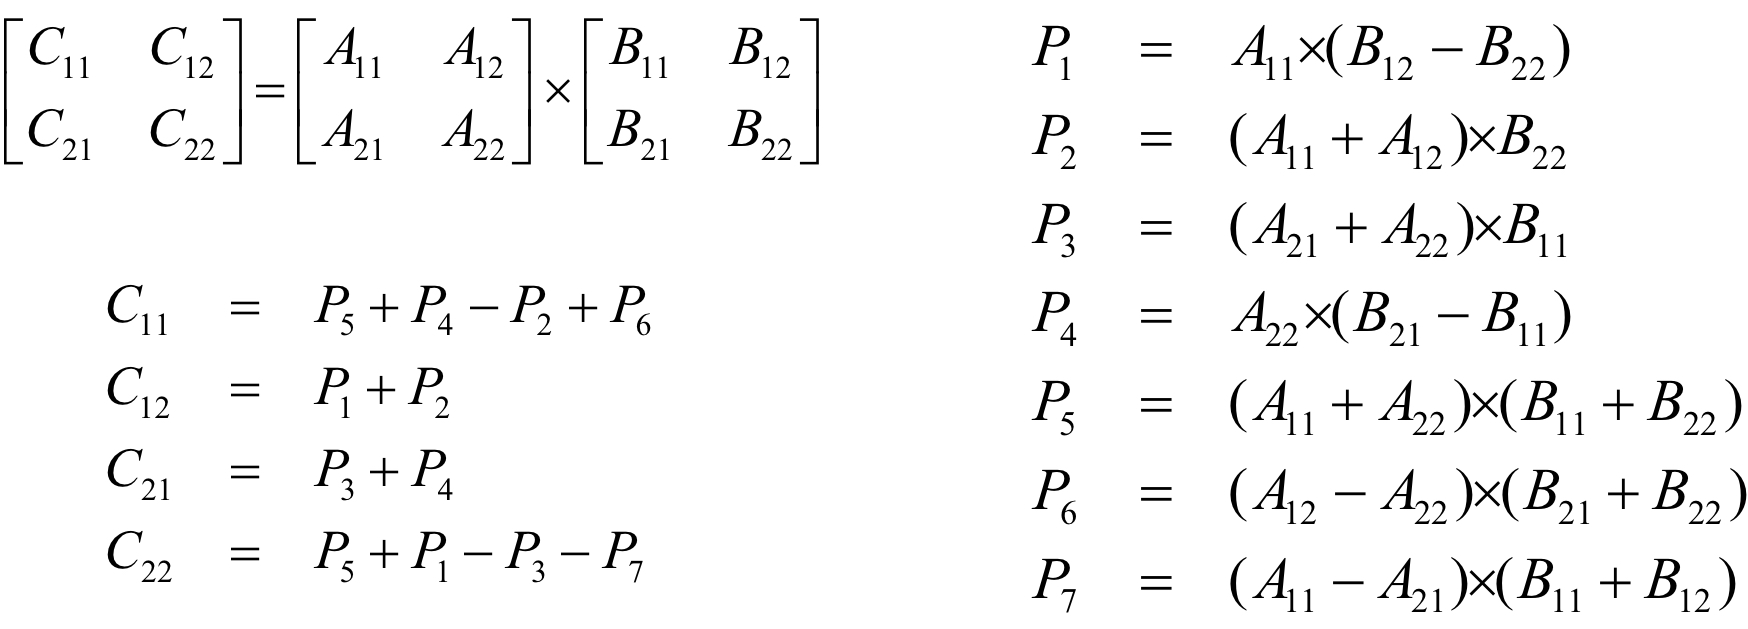
\includegraphics[scale=0.19]{images/02-matrix-mult.jpg}
    \end{center}
    
    And this reduce the running time down to 
    $O(n^{\log_2 7})\approx O(n^{2.807})$.

    Again, many people are trying to reduce the time complexity 
    and another competition arose. 
    We would not go into details here.


\end{spacing}


\chapter{Randomized Algorithm}


\begin{spacing}{1.3}
    
    \section{Recap: Probability}

    Here are some commonly used definitions.

    {\bf Expectation: } $\disp \E(X)=\sum i\cdot \Pr(X=i)$

    {\bf Linearity of expectation: } $\E(X+Y)=\E(X)+\E(Y)$, 
    no matter $X$ and $Y$ are independent or not.

    {\bf Indicator random variables:} $X$ only takes 
    0 or 1, which means $\E(X)=\Pr(X=1)$.

    {\bf Example 1}: coin comes up heads with probability $p$ and 
    tails with $1-p$. Find the expectation of flips $X$ 
    until first head is seen.
    \begin{align*}
        \E(X)&=\sum_{j=1}^{\infty} j\cdot \Pr(X=j)\\
        &= \sum_{j=1}^{\infty}j\cdot (1-p)^{j-1}\cdot p\\
        &= \frac{p}{1-p} \sum_{j=1}^{\infty}j\cdot (1-p)^{j}\\
        &= \frac{p}{1-p}\cdot \frac{1-p}{p} =\frac{1}{p}
    \end{align*}

    The last step is somehow mysterious, the brief idea is: 

    $$\left(\sum_{n=1}^{\infty} x^i\right)'=\sum_{n=1}^{\infty}i\cdot x^{i-1}$$

    multiply each side by $x$, and notice the left hand side is the 
    derivative of geometric series, then: 
    $$x\cdot \left(\frac{x}{1-x}\right)'=\sum_{n=1}^{\infty}i\cdot x^{i}$$
    This gives the last step above.

    {\bf Example 2}: Roll two dice. What is the expected total value $X$?

    It is trivial that $\E(X_1)=\E(X_2)=3.5$, then: 
    $$\E(X_1+X_2)=\E(X_1)+\E(X_2)=7$$

    \section{The Hiring Problem}

    Consider we're looking for an assistant and there are $n$ 
    candidates. We would like to hire the best one, so we 
    interview one by one, and if the current one is better than 
    the best one we've seen before, we just fire the previous one 
    and hire the current one.

    \begin{algorithm*}[H]
        \caption{Hire-Assistant($n$)}

        $best\lar 0$

        \For{$i\lar 1$ to $n$}{
            interview candidate $i$

            \If{candidate $i$ is better than $best$}{
                fire $best$

                hire candidate $i$

                $best\lar i$
            }
        }
    \end{algorithm*}

    This algorithm runs fine, but there is one problem that we 
    may hire too many people(worst case $n$) 
    before we finally find the best one,
    so it may cost lots of money to fire old ones.
    In order to make things better, we consider interview the 
    candidates {\it in a random order}.

    \begin{algorithm*}[H]
        \setstretch{1}
        \caption{Hire-Assistant($n$)}

        {\blue{randomly permute all $n$ candidates}}

        $best\lar 0$

        \For{$i\lar 1$ to $n$}{
            interview candidate $i$

            \If{candidate $i$ is better than $best$}{
                fire $best$

                hire candidate $i$

                $best\lar i$
            }
        }
    \end{algorithm*}

    So what is the expected number of hires in the algorithm above?
    Let an indicator variable $X_i$ where: 
    $$X_i=\left\{ 
        \setstretch{0.5}
        \begin{array}{ll}
            1 &, \text{if we hire candidate }i\\
            0 &, \text{if we don't}
        \end{array}
     \right.$$
    
    Then apparently the number of hires $X=X_1+\cdots+X_n$, thus 
    the expected number of hires, $\E(X)=\E(X_1)+\cdots+\E(X_n)$ 
    according to the linearity of expectation.

    Then what is $\E(X_i)$? Since $X_i$ is an indicator variable, 
    $\E(X_i)=\Pr(X_i=1)$. We hire the candidate $i$ if and only 
    if he/she is the best among all first $i$ candidates, and 
    since they are arranged randomly, the probability that the best 
    one among first $i$ candidates is at the last position is $\frac{1}{i}$.
    Thus, $\E(X_i)=\frac{1}{i}$, and 
    $$\E(X)=\E(X_1)+\cdots+\E(X_n)=1+\frac{1}{2}+\cdots+\frac{1}{n-1}+\frac{1}{n}
    =\Theta(\log n)$$

    \section{Generating a random permutation}

    Notice that in the hiring problem above, we first need to randomly
    permute those candidates. But how can we do that? 
    (Here randomly means all permutations, in total $n!$, should 
    appear with equal probability $\frac{1}{n!}$)

    Let's first look at the implementation of this algorithm, and 
    then explain why it can perform the job well. 
    Assume out computer has a procedure $Random(i, j)$ that can  
    generates a {\bf random uniform} integer between $i$ and $j$.
    ({\bf uniform} means each int occurs with same probability)

    \begin{algorithm*}
        \caption{RandomPermute($A$)}

        $n\lar A.length$

        \For{$i\lar 1$ to $n$}{
            swap $A[i]$ with $A[Random(1, i)]$
        }
    \end{algorithm*}

    \begin{center}
        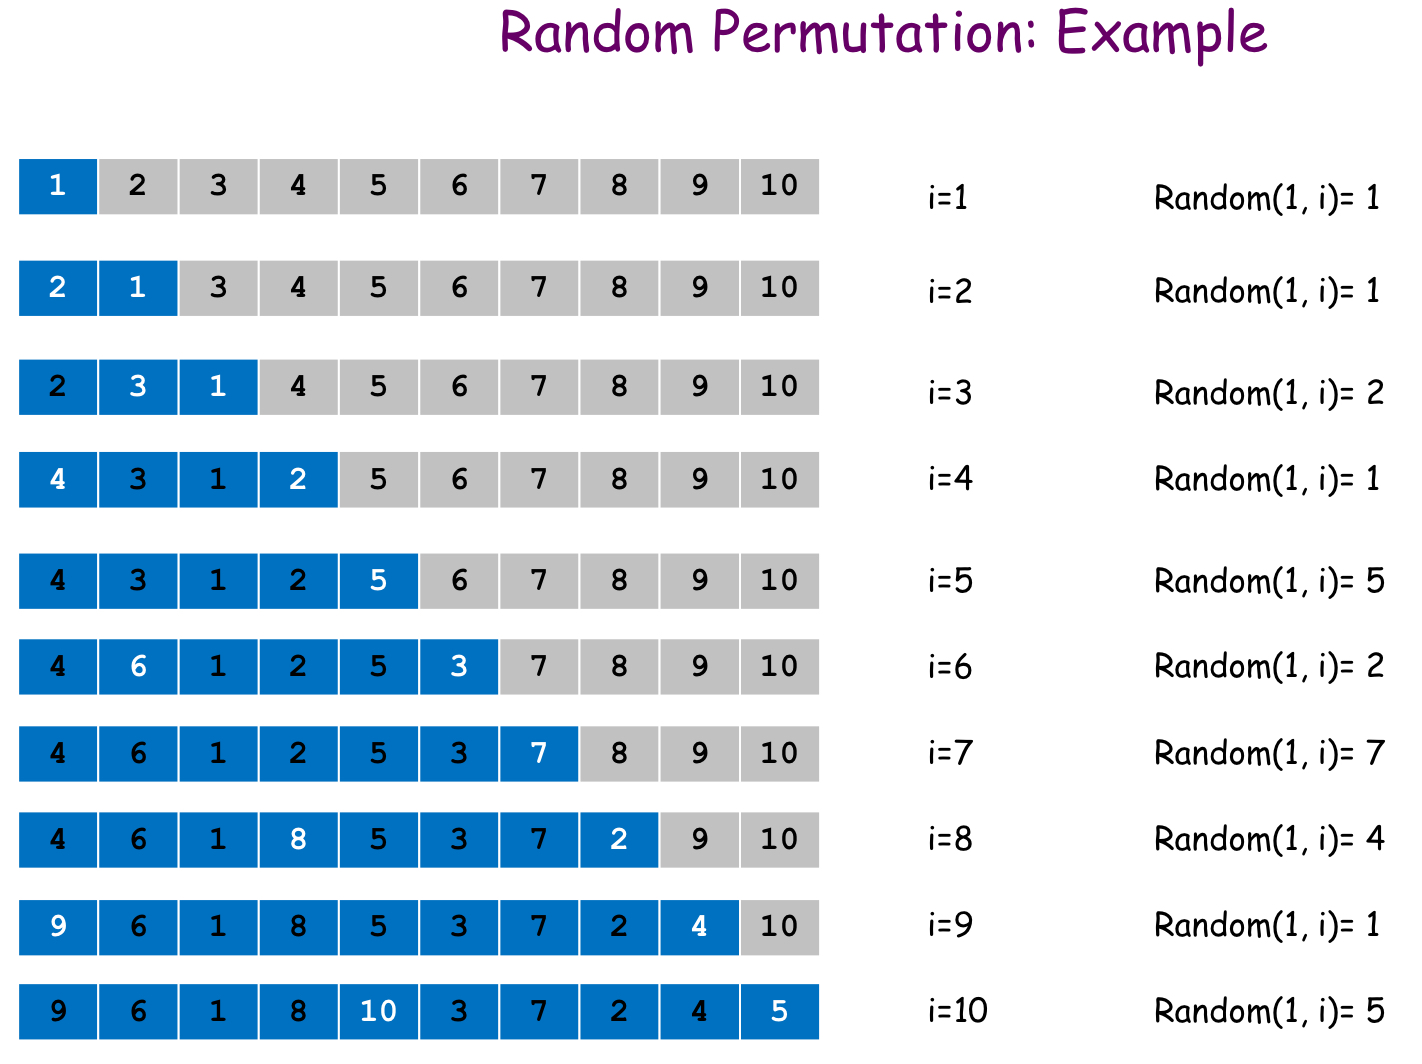
\includegraphics[scale=0.2]{images/03-permutation-eg.jpeg}
    \end{center}

    In the example above, take the last step as an example, 
    the random number we generated is 5, so we will 
    swap the item at index 5, which is 5, with the last item 
    10. Then 10 ends up with index 5 and 5 ends up with index 10.

    Notice this process is actually {\it revertible}, 
    from the end to beginning. For example, we notice at the end, 
    $A[5]=10$, so the last step we must have swapped $A[5]$ with 
    $A[10]$, since before last step, $A[10]=10$. Then if we 
    ``revert'' this step, i.e., swap $A[5]$ and $A[10]$, then 
    the array will back to the status before last step.

    Then, if we denote the random number generated at step $i$
    to be $r_i$, the $n$-tuple $(r_1,\cdots, r_n)$ will 
    generate a permutation of the array. Moreover, given the 
    result permutation, we can actually ``revert'' the process, 
    like we discussed above, to get the $(r_1,\cdots,r_n)$ 
    generated. This means, a tuple $(r_1,\cdots, r_n)$ is 
    {\bf uniquely corresponding} to a permutation at last.
    So if two tuples are different, the permutations they 
    generate are different as well!

    Now we can easily prove the correctness of this algorithm, 
    since each tuple is generated with probability $\dfrac{1}{n!}$,
    (each $r_i$ is generated with probability $\dfrac{1}{n}$),
    then each permutation is also generated with probability 
    $\dfrac{1}{n!}$.

    \vspace{0.3in}

    Here we will give another proof by induction, to show 
    that ``after the $i$-th iteration, $A[1\cdots i]$
    has been randomly permuted.''

    {\bf Base case: }$i=1$, trivial.

    {\bf Inductive step:} Assume $A[1\cdots i-1]$ has been randomly 
    permuted after $i-1$ iterations of the algorithm, then 
    we will calculated the probability that $A[1\cdots i]=
    (a_1,\cdots,a_i)$ appears after the $i$-th iteration.

    For example, if $i=10$, then after $(i-1)$ steps, 
    the array must be something like this: 
    $$[2,8,{\blue 7},3,4,1,5,6,9,{\blue 10}]$$
    then what is the probability that we generate 
    $[2,8,{\blue 10},3,4,1,5,6,9,{\blue 7}]$ after $i$-th step? 
    We must swap $A[3]=7$ with $A[10]=10$, which means 
    $Random(1, i)$ must return 3 to achieve that.

    To summarize the above paragraph, we can get 
    $A[1\cdots i]=(a_1,\cdots,a_i)$ after $i$-th iteration 
    {\it if and only if}
    \begin{itemize}
        \item $Random(1,i)$ returns a specific number and 
        \item $A[1\cdots i-1]$ is a specific $(a_1,\cdots,a_{i-1})$
    \end{itemize}

    The second point above has a probability $\dfrac{1}{(i-1)!}$ according 
    to assumption of induction, the first point above has a probability 
    $\dfrac{1}{i}$. Hence, the probability that $A[1\cdots i]=(a_1,\cdots,a_i)$
    is $\dfrac{1}{(n-1)!}\cdot \dfrac{1}{i}=\dfrac{1}{i!}$, which 
    means that it's a random permutation.

    \section{Quick Sort}

    {\bf Quick Sort} is somehow similar to {\bf Merge Sort}. Instead, 
    it chooses a {\bf pivot} each time, and then {\bf partitions}
    the array so that all items less than or equal to the pivot are 
    on the left and all items greater than pivot are 
    on the right.

    Then it recursively calls QuickSort to left and right sides.

    \begin{algorithm*}
        \caption{QuickSort($A$, $l$, $r$)}

        \If{$l\ge r$}{
            return
        }
        $pivot\lar $ Partition($A$, $l$, $r$)

        QuickSort($A$, $l$, $pivot - 1$)\qquad \tcp{quick sort left part}

        QuickSort($A$, $pivot+1$, $r$)\qquad \tcp{quick sort right part}
    \end{algorithm*}

    For the {\bf Partition} process, we need to choose a pivot first, 
    here we simply choose the last element as pivot. 
    Then we divide the array $A[l\cdots r]$ into two parts: 
    $A[l\cdots i]$ are all smaller or equal than pivot $A[r]$, $A[i+1\cdots j-1]$
    are all larger than pivot $A[r]$, while $A[j\cdots r-1]$ 
    are not decided yet.

    To divide, we perform ``swaps'': iterate $j$ from $l$ to $r-1$,
    if $A[j]$ is smaller or equal than pivot $A[r]$, we expand 
    the area of left part, i.e., $i\lar i+1$, and then swap 
    $A[j]$ with $A[i]$. This will enlarge smaller subpart by size 1, 
    and put the newly found item into that part.
    On the contrary, if $A[j]$ is larger than pivot, then we 
    just expand the larger subpart by size 1, say $j\lar j+1$,
    and no need to do other stuff since $A[j]$ will be already 
    contained after we expand the part.

    Here is the implementation of this process: 

    \begin{algorithm*}
        \caption{Partition($A$, $l$, $r$)}

        $x\lar A[r]$ \qquad \tcp{choose last item to be pivot}

        $i\lar l - 1$\qquad \tcp{No item found yet, so there should be nothing in $A[l\cdots i]$}

        \For{$j\lar l$ to $r-1$}{
            \If{$A[j]\le x$}{
                $i\lar i + 1$   \qquad \tcp{expand left part}

                swap $A[i]$ and $A[j]$ \qquad \tcp{include the new item into left part}
            }
        }
        swap $A[i+1]$ and $A[r]$ \qquad \tcp{make pivot to be at middle}

        return $i+1$    \qquad \tcp{return pivot}
    \end{algorithm*}

    \begin{center}
        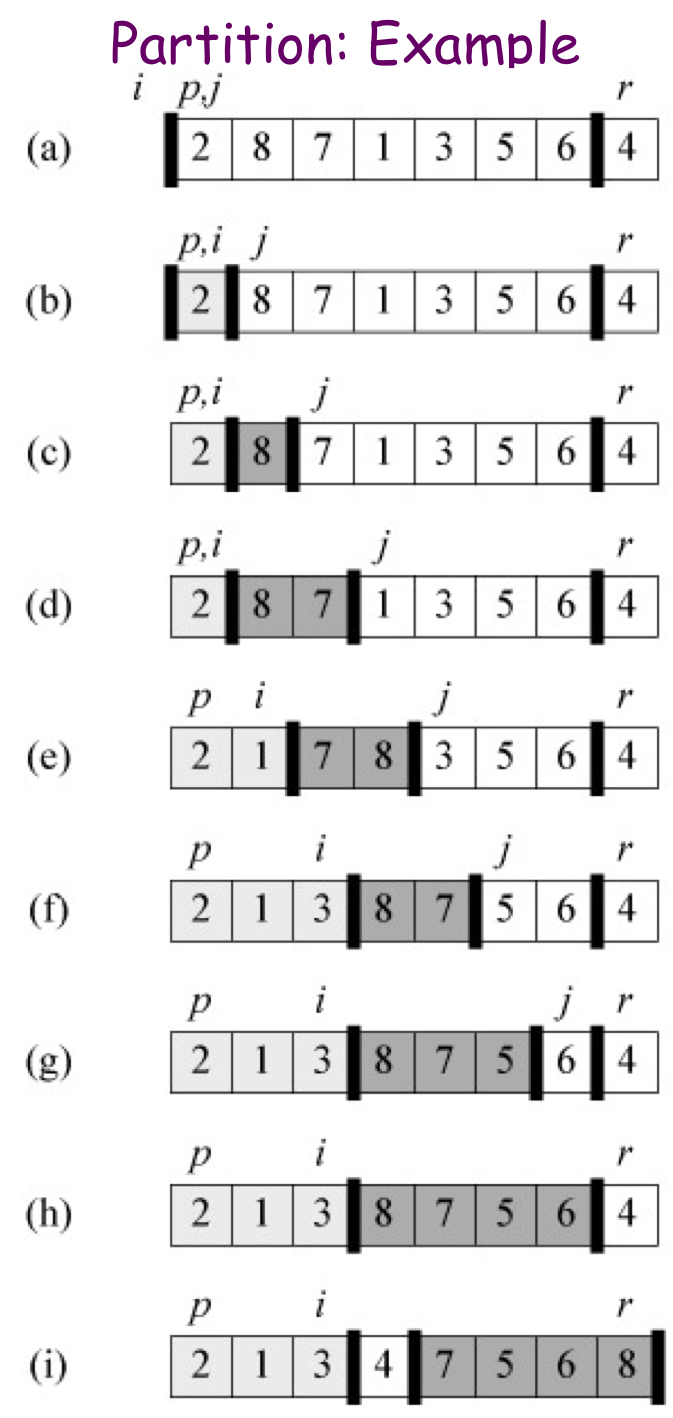
\includegraphics[scale=0.2]{images/03-partition-eg.jpeg}
    \end{center}

    Now we would like to analyze the running time of Quick Sort.
    Firstly, for the best case, where we {\it can always 
    select median element as pivot}, we can divide the array 
    into two parts every time, which gives $\Theta(n\log n)$.
    However, for the worst case, for example, if we always select 
    the smallest(or largest) element as pivot, then 
    it will be $\Theta(n^2)$.

    Thus, in reality, we {\bf randomly} choose a pivot in the 
    array, and this is {\bf randomized algorithm}: making 
    a random choice each time it chooses a pivot.

    For quick sort, or a randomized algorithm, we often care about 
    its {\bf expected running time}, denote as $\E[T(I,R)]$, 
    where $I$ is the input(the array in quick sort), while $R$ is 
    a random string or numbers that decide what we choose as 
    random each time.

    Without loss of generality, we can assume all elements are 
    distinct, since if this is not the case, we can regard 
    original input $A[1\cdots n]$ as $B[1\cdots n]$, where 
    $B[i]=\{A[i], i\}$. Then all elements in $B$ are distinct 
    and we can just manipulate on $B[]$ instead. 
    Also, remember the running time is {\it proportional to}
    number of comparisons. Notice that for any two items, 
    they will either not be compared, or be compared only once,
    that is when one of them is the pivot.
    Since any two items can {\it at most compare once},
    we can define indicator random variable: 
    \begin{align*}
        \setstretch{0.5}
        X_{ij}=\left\{ 
            \begin{array}{ll}
                1 &, {\rm if\ } i{\rm -th\ smallest\ item\ is\ ever\ compared 
                \ with\ }j{\rm -th\ smallest\ item}\\
                0 &, otherwise
            \end{array}
        \right.
    \end{align*}

    Then,
    \begin{align*}
        \E(runtime)&\le \E\left(c\cdot \left(\sum_{i<j}X_{ij}\right)\right)\\
        &=c\cdot \sum_{i<j} \E(X_{ij})\\
        &=c\cdot \sum_{i<j} \Pr(X_{ij}=1)
    \end{align*}
    
    So now we consider how to find $\Pr(X_{ij}=1)$, that is, 
    the probability of $i$-th smallest and $j$-th smallest 
    elements are ever compared. 
    (In the image below, assume items are arranged in 
    ascending order)
    \begin{center}
        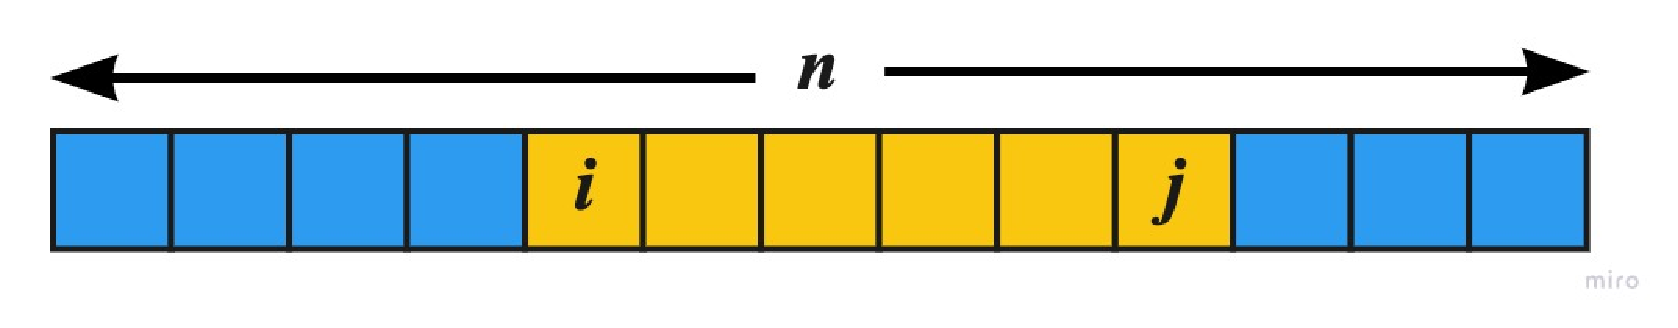
\includegraphics[scale=0.3]{images/03-quicksort-exp.pdf}
    \end{center}
    In the image above, we divide the array into two color regions,
    where between $i$ and $j$(including $i$ and $j$) are colored 
    with yellow.
    \begin{itemize}
        \item if pivot is in {\bf blue region}, then $i$ and $j$
        will be then allocated to the same subpart of array,
        during this process, they cannot be compared to each other.
        \item if pivot is in {\bf yellow region}, then this 
        level is the last chance for $i$ and $j$ to be compared.
        And moreover, $i$ and $j$ will be compared {\it if and 
        only if} $i$ or $j$ is chosen to be the pivot this level.
    \end{itemize}
    Thus, either they will be compared or not is {\it decided 
    at the level which pivot is chosen in yellow region}.
    And at that level, they will be compared if and only if 
    one of them is chosen as the pivot. Therefore,
    $$\Pr(X_{ij}=1)=\frac{2}{j-i+1}$$

    Now we can calculate:
    $$\E(runtime)=c\cdot \sum_{i<j}\E(X_{ij})=c\cdot 
    \sum_{i=1}^{n-1}\sum_{j=2}^{n} \frac{2}{j-i+1}$$

    The summation is hard to calculate directly, but let's make a table: 

    When $i=1$, $\disp \frac{1}{2}+\frac{1}{3}+\frac{1}{4}+
    \cdots+\frac{1}{n-2}+\frac{1}{n-1}+\frac{1}{n}$

    When $i=2$, $\disp \frac{1}{2}+\frac{1}{3}+\frac{1}{4}+
    \cdots+\frac{1}{n-2}+\frac{1}{n-1}$

    When $i=3$, $\disp \frac{1}{2}+\frac{1}{3}+\frac{1}{4}+
    \cdots+\frac{1}{n-2}$

    $\cdots$

    When $i=n-1$, $\disp \frac{1}{2}$

    To sum up {\it by column}, we get: 
    $$(n-1)\cdot \frac{1}{2}+(n-2)\cdot \frac{1}{3}+
    (n-3)\cdot \frac{1}{4}+\cdots +1\cdot \frac{1}{n}$$

    And with some tricks: 
    \begin{align*}
        &\quad (n-1)\cdot \frac{1}{2}+(n-2)\cdot \frac{1}{3}+
        (n-3)\cdot \frac{1}{4}+\cdots +1\cdot \frac{1}{n}\\
        &\le n\cdot \frac{1}{2}+n\cdot \frac{1}{3}+
        n\cdot \frac{1}{4}+\cdots +n\cdot \frac{1}{n}\\
        &= n\cdot \left(\frac{1}{2}+\frac{1}{3}+
        \frac{1}{4}+\cdots \frac{1}{n} \right)\\
        &\le n\cdot \int_1^{n} \frac{1}{x}\ dx= n\ln n
    \end{align*}
    Despite the constant $c$, the expected running time 
    for quick sort is still $\Theta(n\log n)$.

    \section{Randomized Selection}

    {\bf Problem: }Given an array $A$ of $n$ distinct 
    elements, found the $i$-th smallest element in $A$.


\end{spacing}







\part{Sorting Algorithms}

\chapter{Other Basic Sorting Algorithms (optional)}


\begin{spacing}{1.3}

    {\it Notice: } Insertion sort, merge sort and 
    quick sort have been covered in Topic 00, 02, 03,
    respectively, we will not cover them in this note.

    These two algorithms are not paid much attention during this course.
    Selection Sort is introduced in first class which is designed to give students
    an intuition of algorithm, while Bubble Sort is introduced in Tutorial session.
    
    \section{Selection Sort}

    This is quite a natural algorithm: to sort an array of elements, firstly, you
    find the smallest item in the array, put it to first position, and 
    find the smallest item in remaining of the array(i.e., except for the 
    first element), and put it to the second position.

    The real implementation of Selection Sort is just like this, only one thing 
    to amend is that when we find the smallest one and put it to first position, 
    what should we do to the original item that at 1st position? 
    There are two different methods:
    \begin{enumerate}
        \item We put sorted items into a new array, i.e., each time we find the smallest 
        item, we insert it into the new array, so the new array will be sorted
        \item Or, we directly swap the two items. For example, if the smallest 
        item is at position 4, we swap $A[1]$ and $A[4]$. This will not affect 
        our later processes.
    \end{enumerate}
    Apparently, first method is simple but requires extra {\bf space complexity}
    (remember this word?), so usually we choose the second one.

    Let's have an example for this algorithm:
    \begin{itemize}
        \item to sort array: $(5,2,8,6,1)$ 
        \item 1st step: find the smallest one, $1$, swap with first item, 
        results in $(1,2,8,6,5)$
        \item 2nd step: find the smallest except for first item, $2$, swap with second item, 
        results in $(1,2,8,6,5)$
        \item 3rd step: find the smallest except for first two items, $5$, swap with third item, 
        results in $(1,2,5,6,8)$
        \item $\cdots$
    \end{itemize}

    The pseudocode should be like this:
    \begin{algorithm*}[htbp]
        \caption{Selection-Sort-1($A[1\cdots n]$)}

        \For{$i\lar 1$ to $n-1$}{
            \tcp{Now we want to find the smallest item among $A[i\cdots n]$}

            $minNum\lar A[i]$ \qquad \tcp{Records the smallest item we've met}

            $minIndex\lar i$\qquad \tcp{Records the index of $minNum$}

            \For{$j\lar i+1$ to $n$}{
                \tcp{If a smaller one found, record it!}
                \If{$A[j] < minNum$}{
                    $minNum\lar A[j]$

                    $minIndex\lar j$
                }
            }

            \tcp{After finding the smallest one, swap with $A[i]$}

            swap $A[i]$ and $A[minIndex]$
        }
    \end{algorithm*}

    The lecture slides use a different implementation, instead of looking 
    for the smallest one and, at the end, swap it with current one($i$-th item), 
    we continuously swap $A[i]$(current one) and $A[j]$ whenever we find 
    such an $A[j]$ that smaller than $A[i]$. For example, to sort $(5,2,8,6,7,1)$,
    \begin{itemize}
        \item First $i=1$, $A[i]=5$, and we loop $j$ from $2$ to $6$, to check if there 
        is a smaller item 
        \item when $j=2$, $A[j]=2<A[i]=5$, we swap them, results in $({\red 2},{\red 5},8,6,7,1)$
        \item when $j=3$, $A[j]=8>A[i]=2$, don't swap
        \item when $j=4$, $A[j]=6>A[i]=2$, don't swap
        \item when $j=5$, $A[j]=7>A[i]=2$, don't swap
        \item when $j=6$, $A[j]=1<A[i]=2$, swap them, results in $({\red 1},5,8,6,7,{\red 2})$
    \end{itemize}

    The pseudocode of this algorithm looks much shorter, but actually their thoughts 
    and time complexity don't differ too much.
    \begin{algorithm*}[htbp]
        \caption{Selection-Sort-2($A[1\cdots n]$)}

        \For{$i\lar 1$ to $n-1$}{
            \For{$j\lar i+1$ to $n$}{
                \tcp{Look for smaller item, and swap with $A[i]$}

                \If{$A[i]>A[j]$}{
                    swap $A[i]$ and $A[j]$
                } 
            }
        }
    \end{algorithm*}

    The correctness of {\bf Selection Sort} can be proved by induction.
    \begin{theorem}
        When {\bf Selection Sort} terminates, the array is sorted.
    \end{theorem}
    \begin{proof}
        We use induction to prove it.

        {\bf Basic step:} When $n=1$, the algorithm is obviously correct.

        {\bf Inductive step:} Assume the algorithm sorts {\it every array of size $n-1$} correctly,
        then for an size $n$ array $A[1\cdots n]$, what the algorithm does is that:
        \begin{itemize}
            \item It first find the smallest item, and put it at $A[1]$
            \item Then, it omits the first item, and runs {\bf Selection Sort} on $A[2\cdots n]$:
            where by induction, this correctly sort $A[2\cdots n]$
            \item Since $A[1]$ is the smallest, the whole array $A[1\cdots n]$ are sorted.
        \end{itemize}
    \end{proof}


    The running time of Selection Sort is easy to analyze. Take the second algorithm above 
    as example, line 3 and line 4 will run for each iteration of the two loops, so 
    the running time is 
    $$\sum_{i=1}^{n-1}\sum_{i+1}^n 1=\sum_{i=1}^{n-1} (n-i)=\frac{n(n-1)}{2}$$
    which immediately follows that the running time of Selection Sort is always $\Theta(n^2)$.

    \section{Bubble Sort}

    The idea of {\bf Bubble Sort} is that: each time we check two adjacent items, 
    if the left one is larger, we swap them. Then, after one iteration through the whole 
    array $A[1\cdots n]$, the largest item will be ``bubbled'' to right-most position.
    Then, we continuously do this on $A[1\cdots n-1]$(except for the last one, which already 
    sorted), and now the second-largest item will be ``bubbled'' to second-rightmost position.

    The pseudocode is like this:
    \begin{algorithm*}[htbp]
        \caption{Bubble-Sort-1($A[1\cdots n]$)}
        \For{$i\lar 1$ to $n$}{
            \tcp{Could you explain why $j$ terminates at $n-i$?}
            \For{$j\lar 1$ to $n-i$}{
                \tcp{Check adjacent, if left is larger, swap them}
                \If{$A[j]>A[j+1]$}{
                    swap $A[j]$ and $A[j+1]$
                }
            }
        }
    \end{algorithm*}

    This algorithm looks stupid, since it requires lots of ``checking and swaps''. Consider the case 
    where the input is already sorted, the {\bf Bubble Sort} algorithm above still 
    perform ALL two nested loops, and check each adjacent items to see if they need swaps.
    Inspired by this, we can directly terminates the algorithm if {\it the previous $j$ iteration 
    does zero swaps}. If the $j$ loops from begin to end and find that no swap is required, then 
    no surprising the array must have already been sorted.
    
    So now we can change the algorithm into:
    \begin{algorithm*}[htbp]
        \caption{Bubble-Sort-2($A[1\cdots n]$)}
        $swapped\lar true$\qquad \tcp{Record whether we swapped last time, here initialize to true}
        \While{$swapped$ is true}{
            $swapped\lar false$
            \For{$i\lar 1$ to $n-1$}{
                \If{$A[i]>A[i+1]$}{
                    swap $A[i]$ and $A[i+1]$

                    $swapped\lar true$
                }
            }
        }
    \end{algorithm*}

    The correctness of Bubble Sort can be obtained by the correctness of below two theorems:
    \begin{theorem}
        When Bubble Sort terminates, the array must be sorted.
    \end{theorem}
    \begin{proof}
        The algorithm terminates only if the last pass did not swap any pair, i.e
        $$A[1] \le  A[2] \le  \cdots \le A[n - 1] \le A[n],$$
        which means that the array is sorted.
    \end{proof}
    \begin{theorem}
        After the $i$-th pass, the items in locations $A[n - i + 1, \cdots , n]$ are in their proper
        sorted locations and none of them ever move again.
    \end{theorem}
    \begin{proof}
        We prove this claim by induction.
        \begin{itemize}
            \item This is obviously true if $n=1$ or $n=2$.
            \item After the 1st pass, the largest element must be in location $A[n]$, 
            and that item never moves after the first pass completes.
            \item After the 1st pass completes, it is as if Bubble Sort is being run on array $A[1 \cdots n-1]$.
            \item The claim then follows by induction.
        \end{itemize}
    \end{proof}


    For time complexity, the best case is when the array is already sorted, $O(n)$, while 
    the worst case is when the array is reversely sorted, $O(n^2)$, the worst case complexity
    can be directly observed from our first Bubble Sort algorithm.

    There is also a formal proof of worst case in problem set SS6. I'd like to omit details here.


    
\end{spacing}


\chapter{Heap Sort}

\begin{spacing}{1.3}
    \section{Intro. to Heap}

    Omitting excessive introductions, now we want a data structure that supports 
    two operations:
    \begin{itemize}
        \item {\bf Insert}: insert a new element into it
        \item {\bf Extract-Min}: removes and returns the smallest element inside
    \end{itemize}

    For now, you may come up with some possible implementations:
    \begin{itemize}
        \item Use a list:
            \begin{itemize}
                \item {\bf Insert} requires $O(1)$ time.
                \item {\bf Extract-Min} requires $O(n)$ time, since you need scan 
                through the list to find the smallest one
            \end{itemize}
        \item Use a sorted list:
            \begin{itemize}
                \item {\bf Insert} requires $O(n)$ time, since in order to 
                maintain the list to be sorted, you need to scan through the list 
                to find a suitable place to insert the new element.(like insertion sort)
                \item {\bf Extract-Min} requires $O(1)$ time, since list is sorted.
            \end{itemize}
    \end{itemize}

    However, we are not satisfied with the results above, let's introduce {\bf Heap}.

    \newpage
    \begin{definition}
        {\bf Heaps} are {\bf binary trees}, with the restrictions:
        \begin{itemize}
            \item 
            \item All levels must be full, except for the lowest level
            \item If the lowest level is not full, all nodes must be packed to the left.
        \end{itemize}
    \end{definition}
    \begin{figure}[htbp]
        \centering
        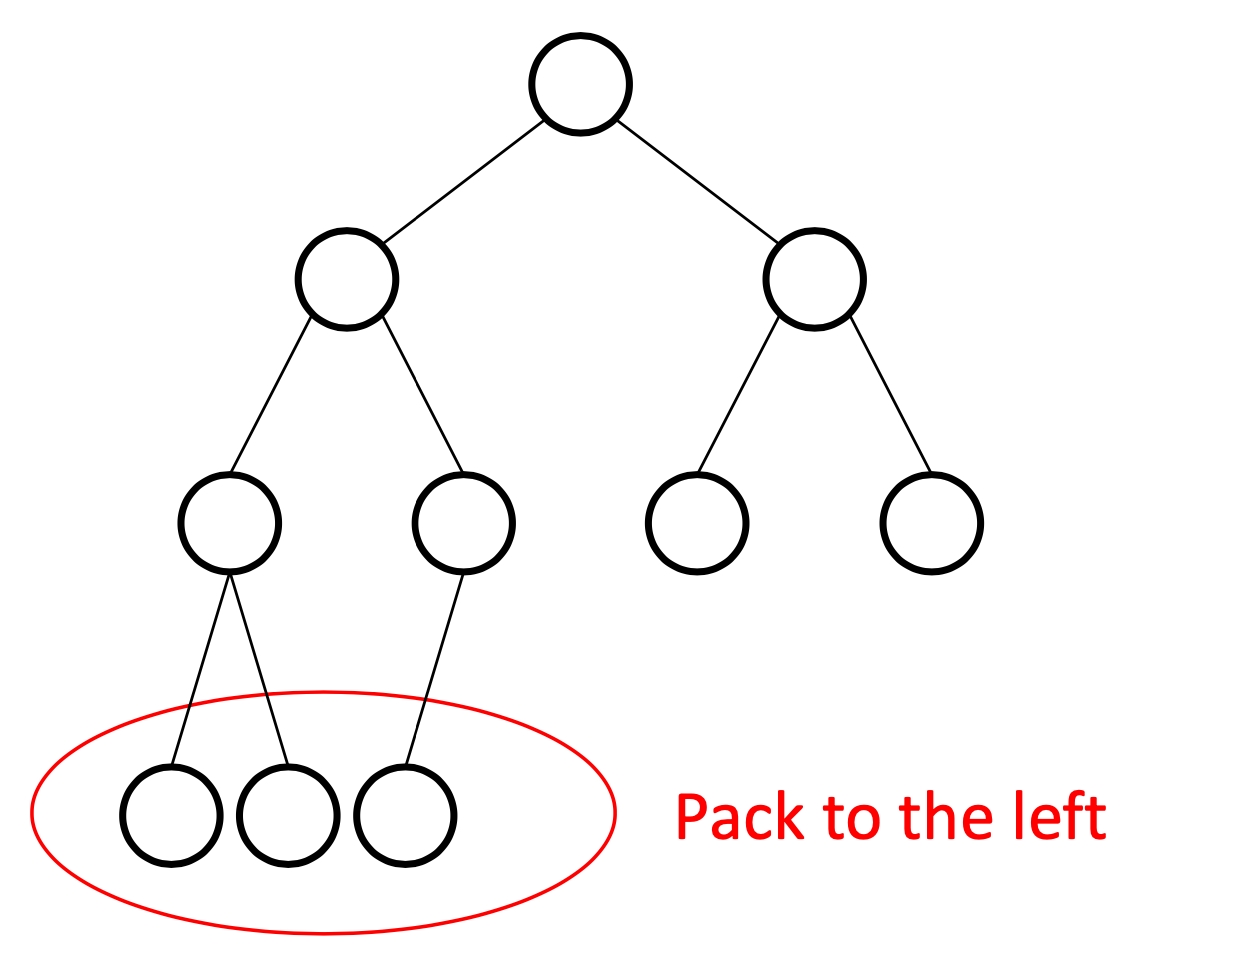
\includegraphics[scale=0.38]{images/05-heap-intro.png}
    \end{figure}

    We also define a special kind of heap called {\bf Min-heap}.
    \begin{definition}
        {\bf Min-heap} is a {\bf heap} in which the value of a node 
        is {\it at least} the value of its parent.
    \end{definition}
    \begin{figure}[htbp]
        \centering
        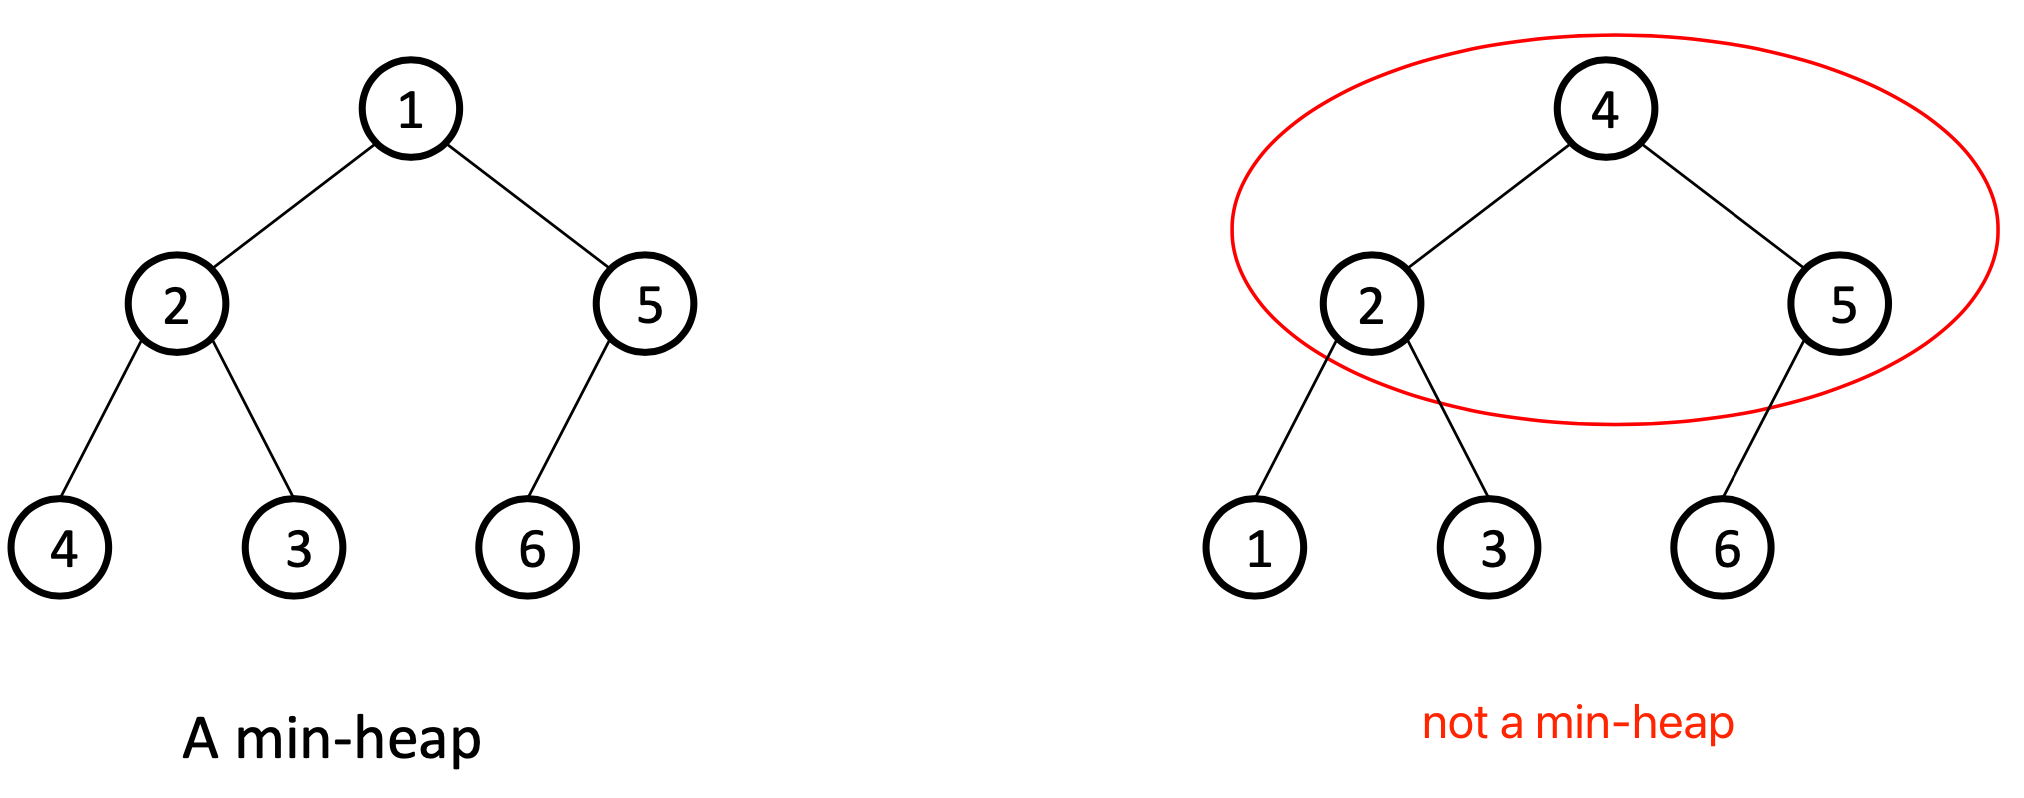
\includegraphics[scale=0.4]{images/05-min-heap-intro.png}
    \end{figure}

    Since {\bf heap} is a special kind of {\bf binary tree}, its height $h$
    and number of elements $n$ are related:
    \begin{theorem}
        For a {\bf heap} with $n$ elements and height $h$, there must be 
        $$2^h\le n<2^{h+1}$$
        thus an $n$-element heap has height $\Theta(\log n)$.
    \end{theorem}
    \begin{proof}
        The proof is trivial, only use the fact that a binary tree with height $h$
        can have at most $2^{h+1}-1$ nodes(height starts from 0), so a heap with 
        height $h$ must have $2^h-1$ nodes before level $h$(since they must be full).
    \end{proof}

    Interestingly, the structure of {\bf heap} is so regular so that we can 
    use an array to represent it.
    \begin{figure}[htbp]
        \centering
        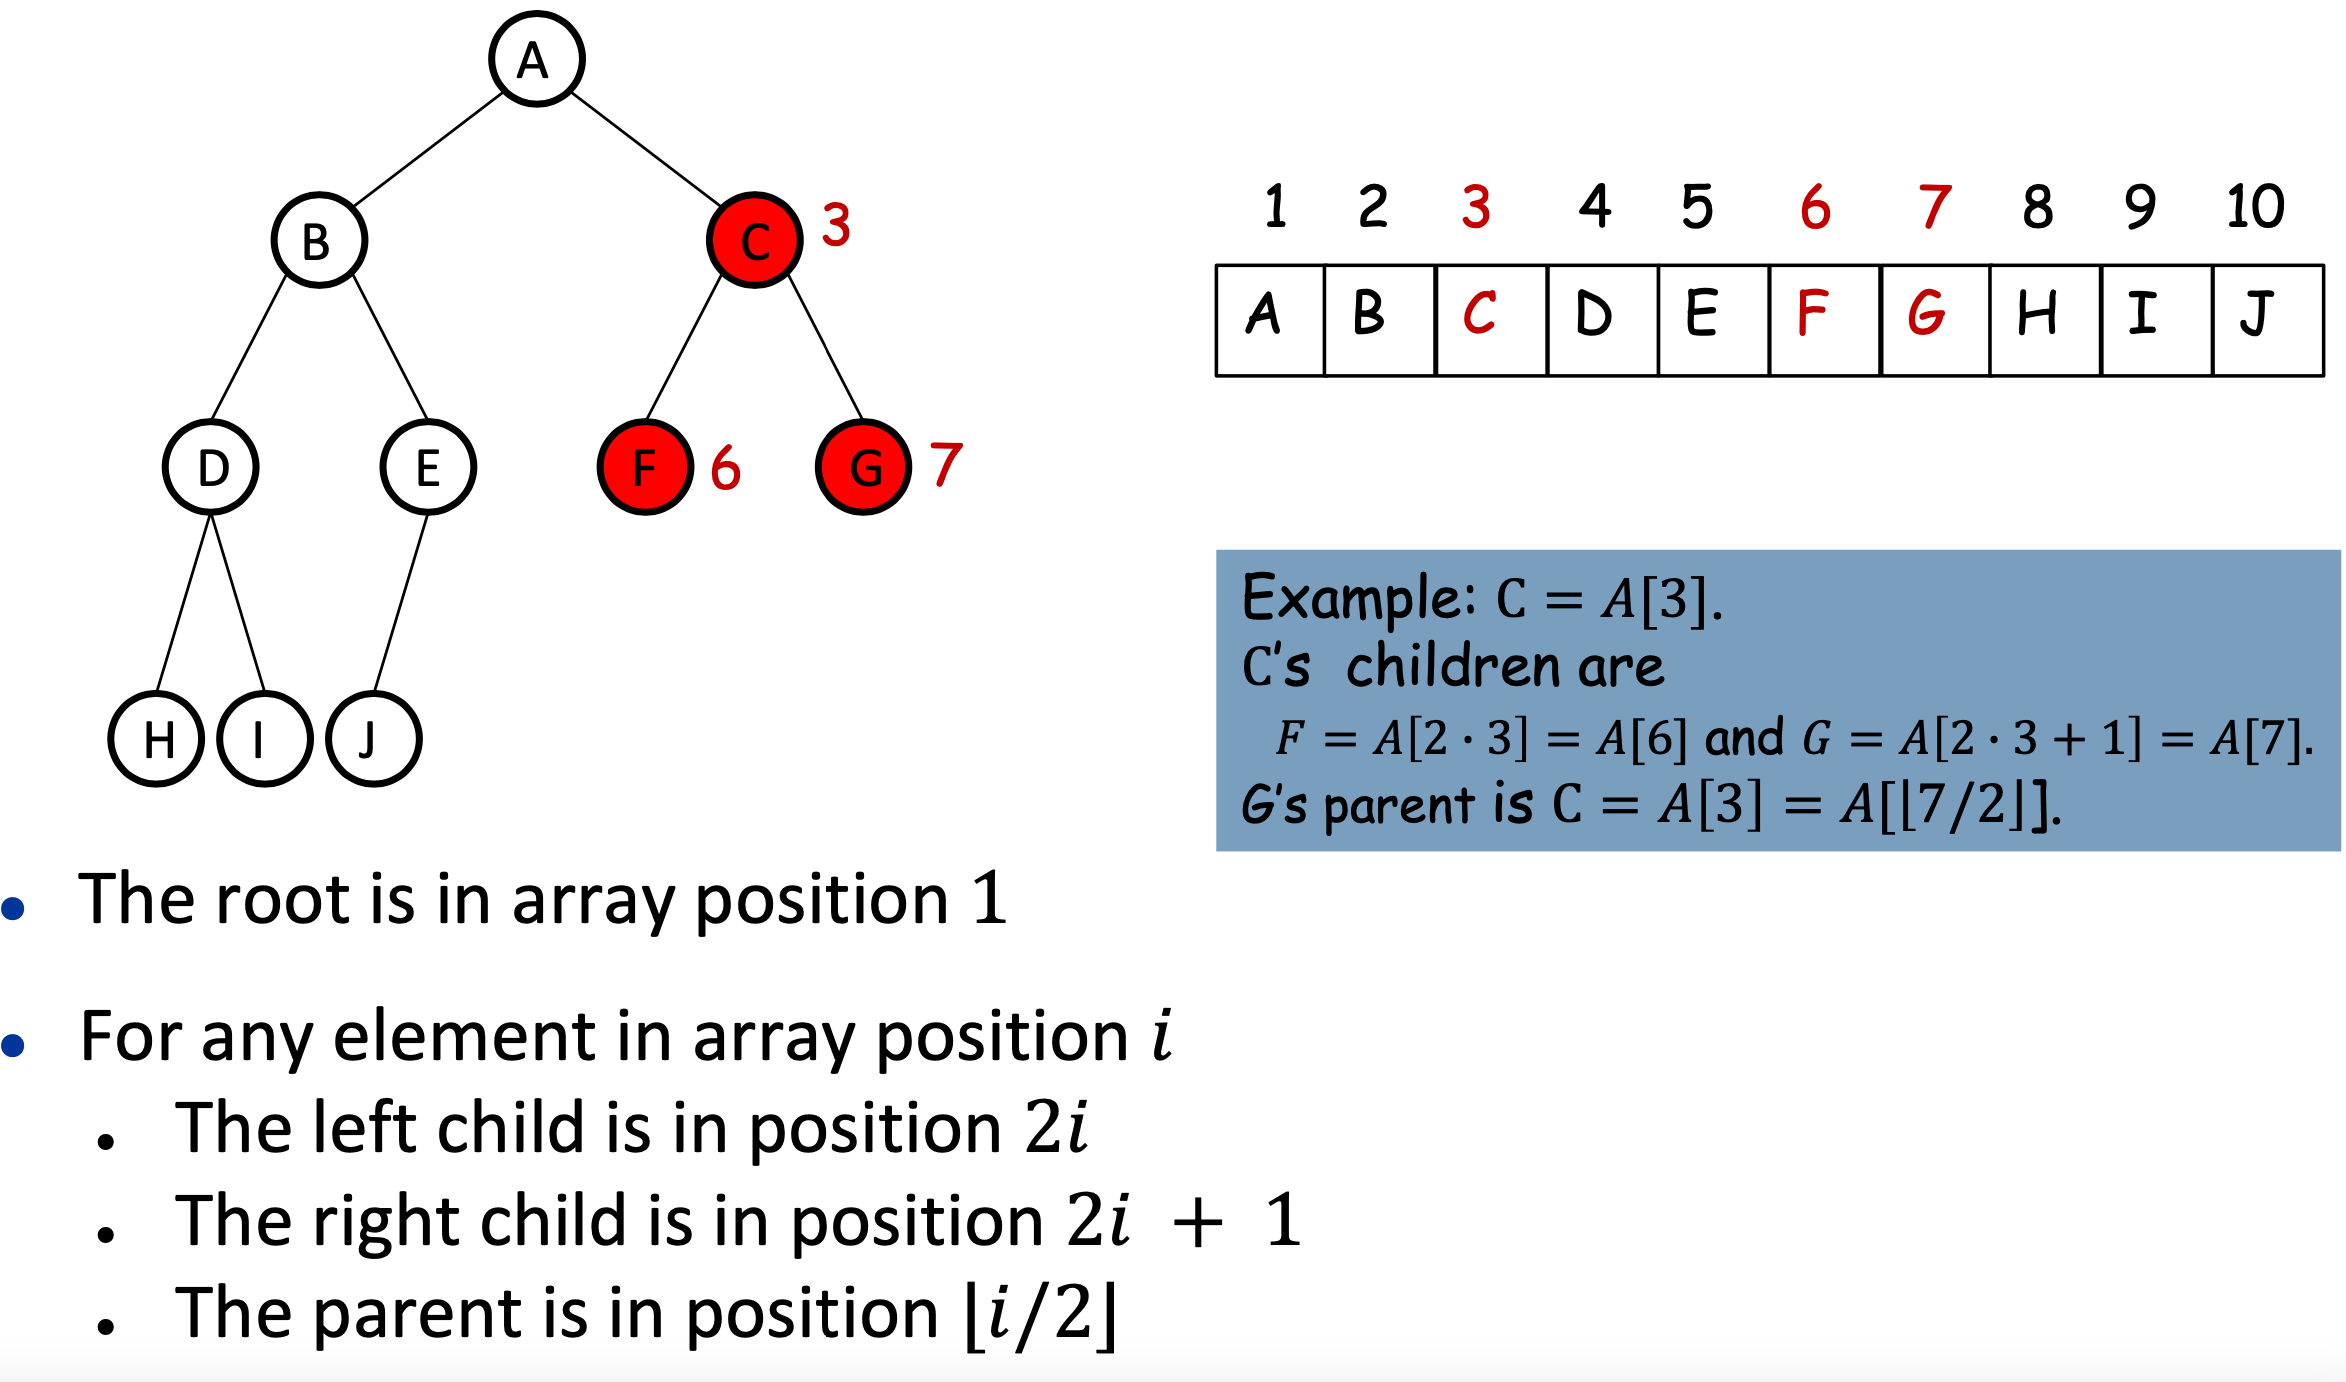
\includegraphics[scale=0.35]{images/05-heap-array.png}
    \end{figure}

    Now with the properties of heap, we can introduce how we can use heap to 
    efficiently perform {\bf insertion} and {\bf extract-min} operations.


    \vspace{0.3in}
    \section{Insertion}

    Recall that a heap must be ``left-packed'', so it is not surprising that 
    if we insert a new node, we should insert it into the {\it next available 
    position at the lowest level}. ``The lowest level'' is because the 
    upper levels are all full, and ``next available'' means the immediate 
    right position of the last node, which allows us to maintain the ``left-packed'' property.

    So if we insert 1 into the heap below, we end up with:
    \begin{figure}[htbp]
        \centering
        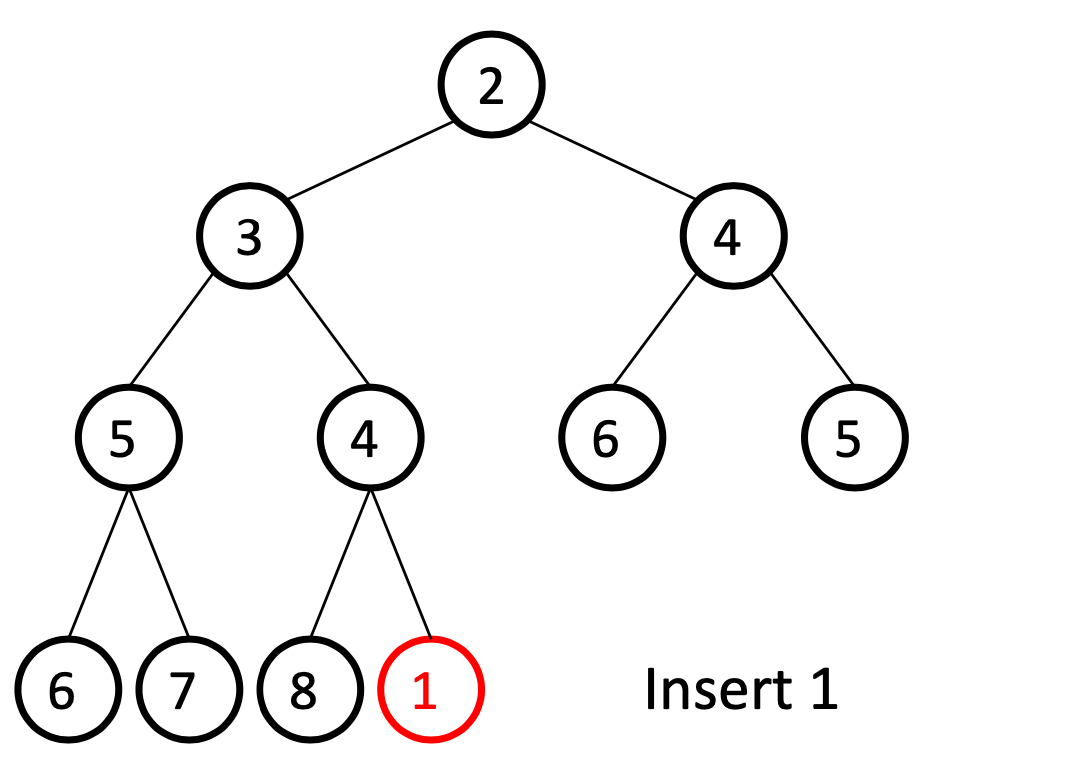
\includegraphics[scale=0.25]{images/05-insert-1.png}
    \end{figure}

    You may have already noticed that the new heap violates the ``min-heap property'', namely
    1 has a parent 4 that is larger than 1. To fix the problem, we consider 
    ``{\bf percolate up(or bubble up)}'': such that if the parent of the node is 
    larger than the node, we swap the parent with that child.

    Here, since $4>1$, we swap parent 4 and its child 1:
    \begin{figure}[htbp]
        \centering
        \qquad 
        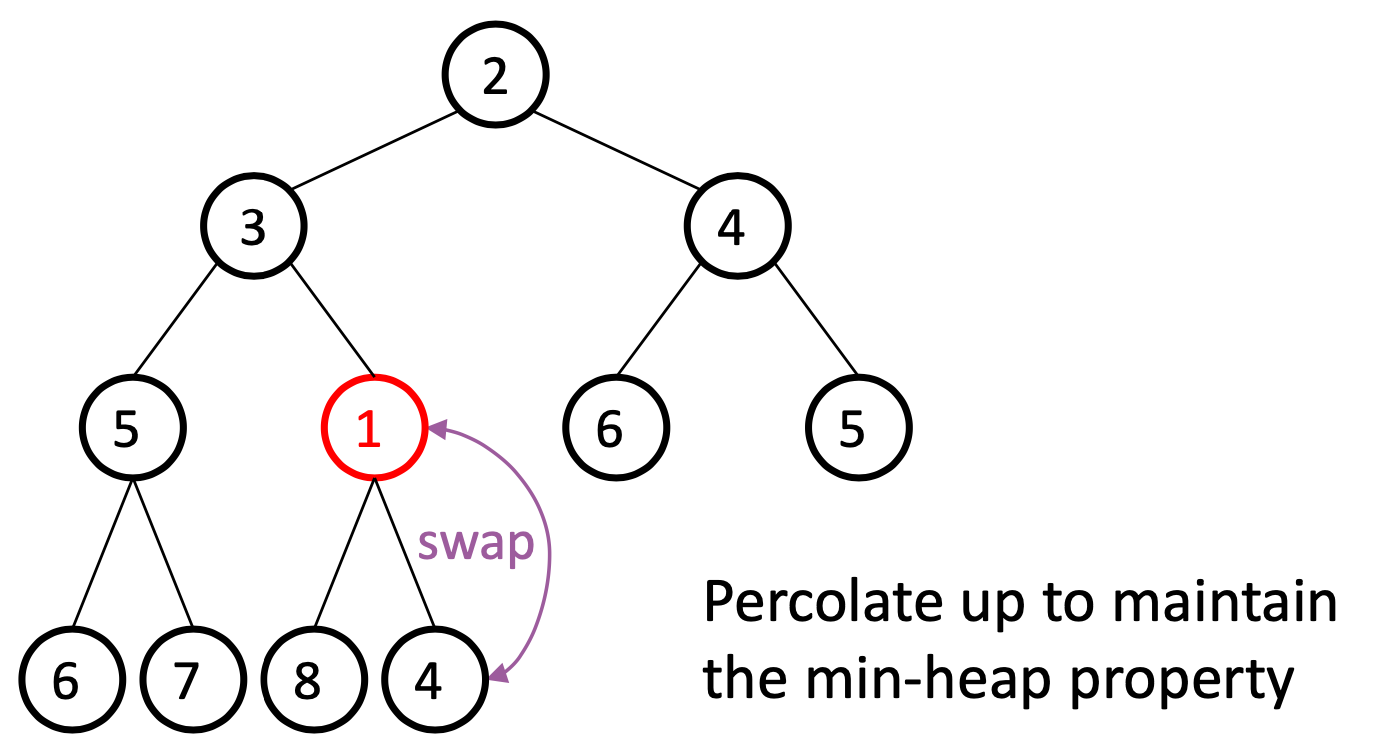
\includegraphics[scale=0.25]{images/05-insert-2.png}
    \end{figure}

    However, 1 still has a parent 3 that larger than 1, so we bubble up again:
    \begin{figure}[htbp]
        \centering
        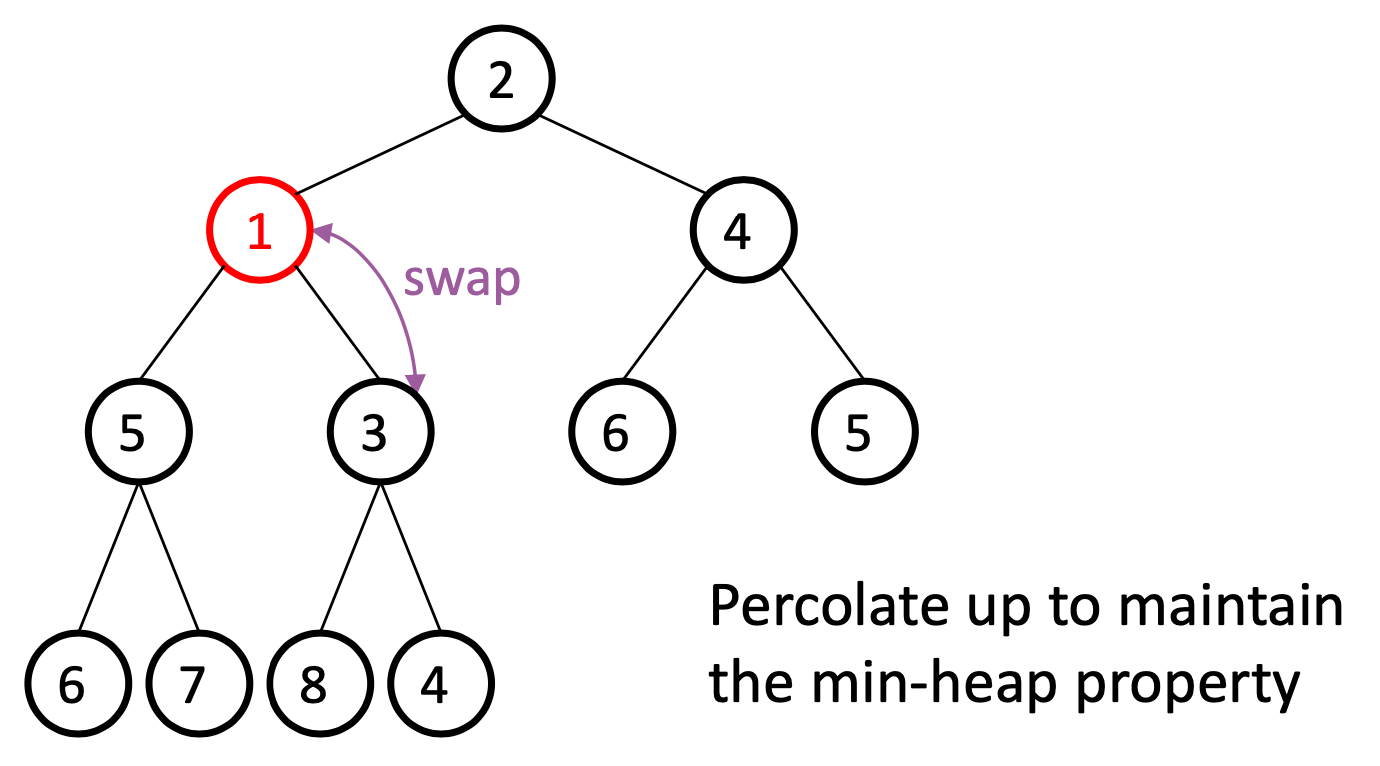
\includegraphics[scale=0.25]{images/05-insert-3.png}
    \end{figure}

    1 still has a parent 2 that larger than 1, bubble up again:
    \begin{figure}[htbp]
        \centering
        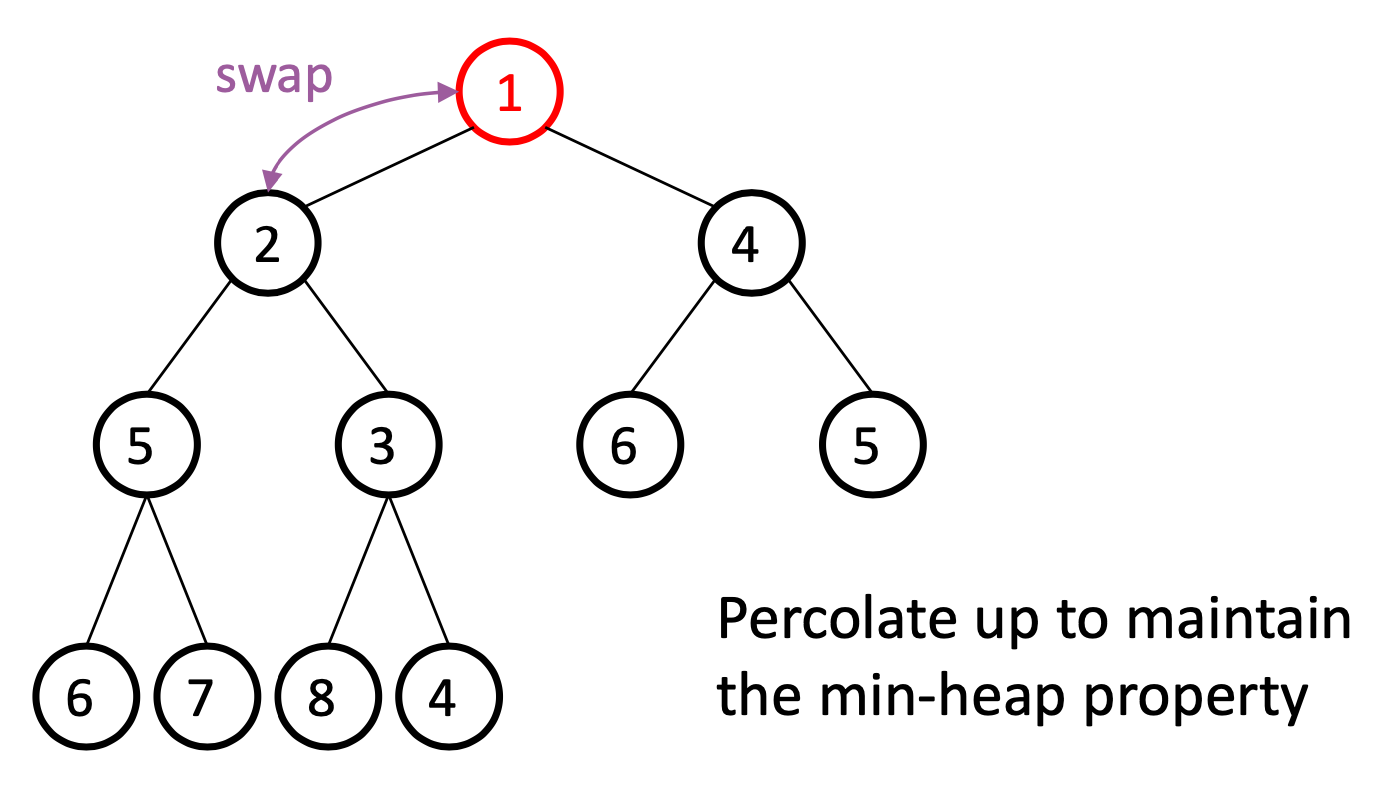
\includegraphics[scale=0.25]{images/05-insert-4.png}
    \end{figure}

    The heap now is fine.

    Since after each swap, the min-heap property is satisfied for the current subtree
    (with the new element as root), so after all those bubble up operations, the 
    min-heap property will certainly be preserved.

    The {\bf time complexity}, which can be measured by number of swaps, is 
    at most the height of heap, i.e., $O(\log n)$.

    We should notice that the swapping process is not necessarily stopped 
    when the new element reaching the top, instead, it stops when 
    its parent is smaller than it. For example, if we insert 2 into the resulted heap above,
    \begin{figure}[htbp]
        \centering
        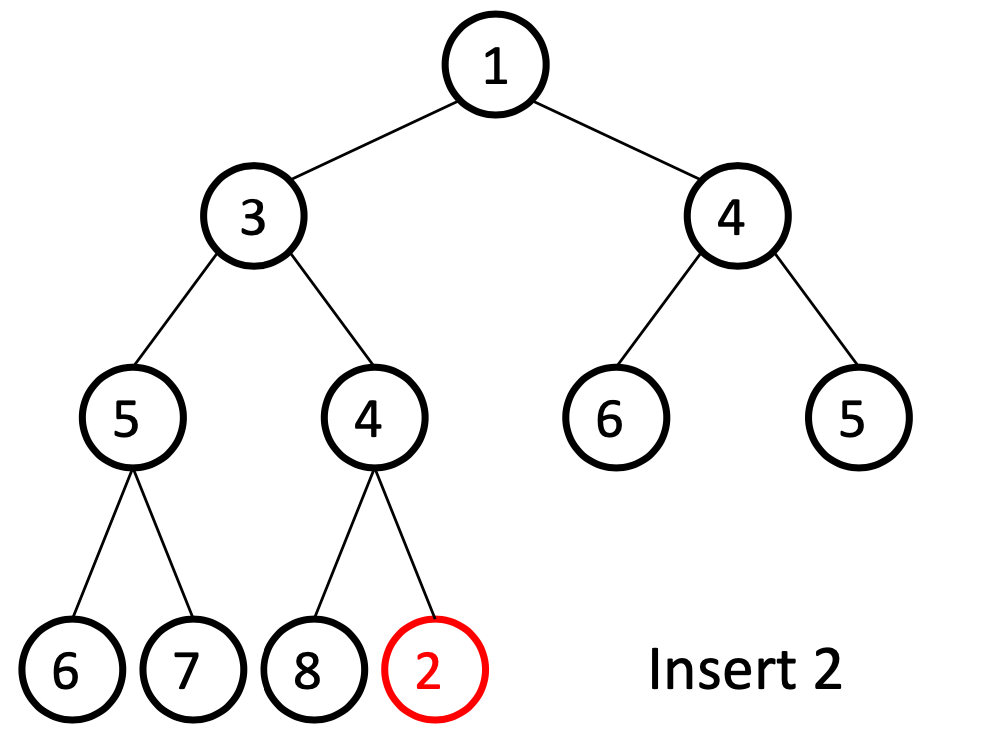
\includegraphics[scale=0.22]{images/05-insert-5.png}\quad 
        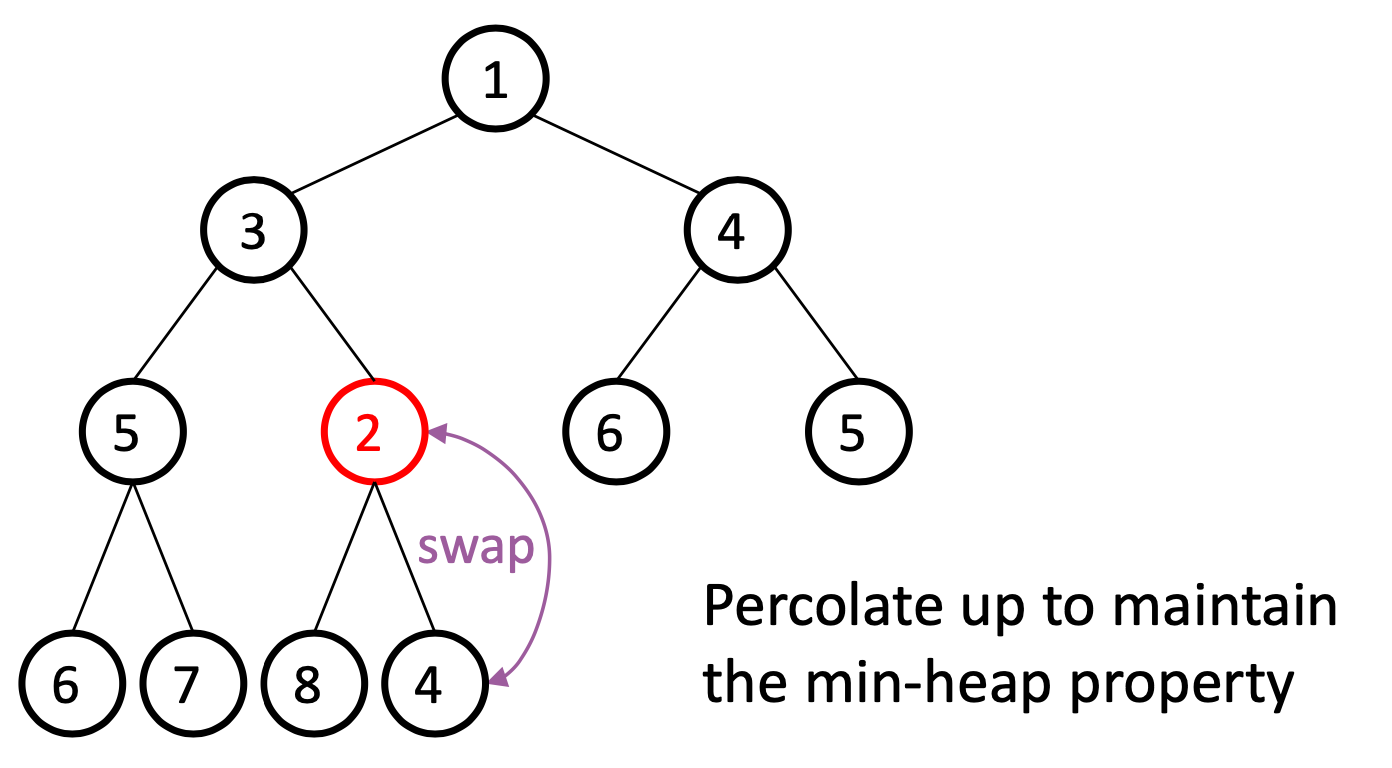
\includegraphics[scale=0.22]{images/05-insert-6.png}\quad 
        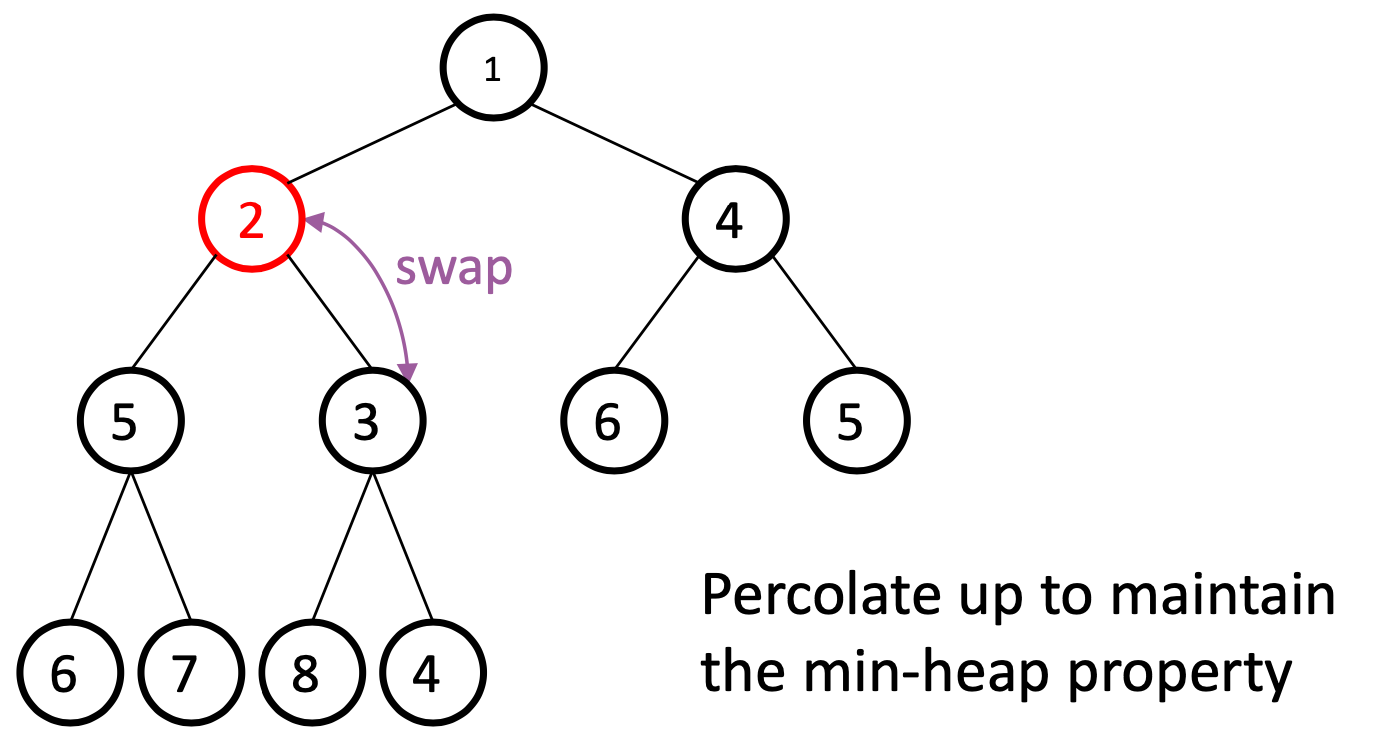
\includegraphics[scale=0.22]{images/05-insert-7.png}\quad 
    \end{figure}
    the process stops before reaching root 1.


    We conclude this section with pseudocode of Insert operation.
    \begin{algorithm*}[htbp]
        \caption{Insert($x$, $i$)}
        \tcp{Insert item $x$ to heap $A[1\cdots i-1]$ creating heap $A[1\cdots i]$}

        $A[i]\lar x$

        $j\lar i$

        \tcp{If smaller than parent, and not reach root yet}
        \While{$A[j]<A\left[\lf \frac{j}{2} \rf\right]$ and $j>1$}{
            \tcp{bubble up $A[j]$, swap with its parent}

            swap $A[j]$ and $A\left[\lf \frac{j}{2} \rf\right]$

            $j=\lf \frac{j}{2} \rf$\qquad \tcp{continue the process on new parent}
        }
    \end{algorithm*}

    \vspace{0.3in}
    \section{Extract-Min}
    
    




\end{spacing}

\chapter{Linear Sort}

\begin{spacing}{1.3}
    \section{Lower Bound for Comparison Sorts}

    So far, all sorting algorithms we have seen perform no better than $\Omega (n \log n)$. 
    You may wonder if it is possible to have a much faster sorting algorithm,
    and the answer is No, if we {\it restricted to comparison sorts}, i.e., each time we 
    compare two numbers and decide some kind of order of them. All sorting algorithm we have seen 
    are {\bf comparison-based} sorts, and we can prove that any sorting algorithm based only on 
    comparison cannot perform better than $\Omega (n\log n)$.

    \begin{theorem}
        Any comparison sort algorithm requires $\Omega (n\log n)$ comparisons in the worst case.
    \end{theorem}

    Note that the correctness of the theorem above directly gives ``$\Omega(n\log n)$ is a 
    lower bound for all {\bf Comparison-Based Sorting} algorithms.''

    To proof the theorem, we first introduce {\bf Decision Tree}, with which we can view 
    the process of comparison sorts. 
    \begin{definition}
        A {\bf decision tree} is a {\it full binary tree} that represents the comparisons between 
        elements that are performed by a particular sorting algorithm on an input of given size.
    \end{definition}
    In a decision tree, each {\it non-leaf} node is represented by $i:j$ to indicate that we are comparing 
    $i$ and $j$, and if $i\le j$, we go to the left subtree, while $i>j$ goes to the right.
    Each {\it leaf} node represents a permutation of the result of sorting algorithm, corresponding to 
    an order of all items.

    The example below can help you have a better understanding of decision tree.
    \begin{center}
        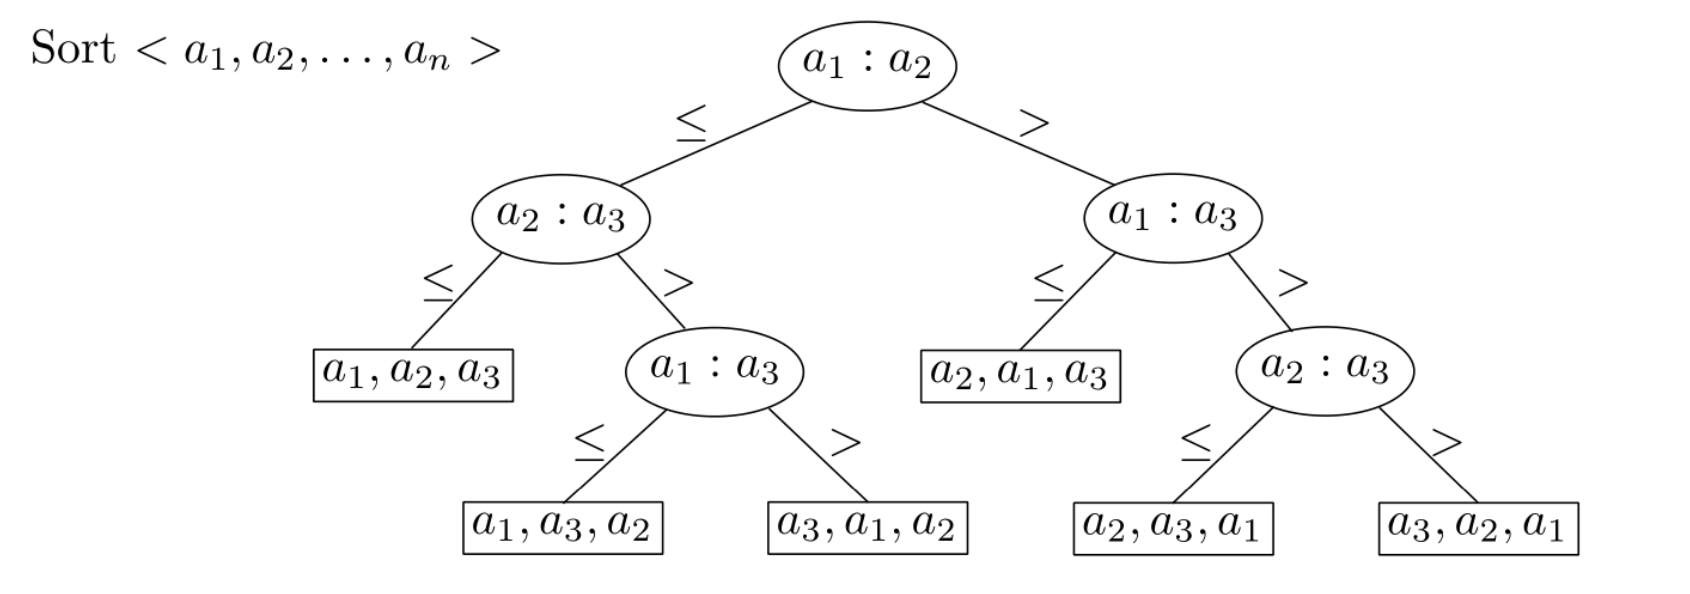
\includegraphics[scale=0.45]{images/06-decision-tree.png}
    \end{center}

    So the decision tree above basically imitates the process of our comparison sort,
    for example, we first ask ``Is $a_1$ larger than $a_2$?'', assuming the answer is 
    No, we go to left subtree, and then ask ``Is $a_2$ larger than $a_3$?'', and if 
    the answer is also No, we go to left subtree again, and reach a leaf node, 
    which means now we can determine their order, which is $a_1\le a_2\le a_3$.

    Notice that any correct sorting algorithm must be able to produce {\it each 
    permutation} of its input, each of the $n!$ permutations of a size $n$ input 
    must appear as one of the leaves of the decision tree for a comparison sort to be correct.
    (think why, though this is intuitive)

    Therefore, the decision tree must have $n!$ leaves since a sorting algorithm 
    can have $n!$ different outputs for each possible permutation on $n$ items.
    Moreover, a binary tree(recall decision tree is binary) with $n!$ leaves must 
    have height $\Omega(\log n)$(see theorem below). Therefore, the height of 
    tree must be 
    $$\Omega (\log (n!))=\Omega(n\log n)$$
    which means we need $\Omega(n\log n)$ comparisons in this algorithm, 
    therefore comparison-based sorting algorithm requires at least $\Omega(n\log n)$ time.

    \begin{theorem}
        A binary tree with $n$ leaves must have height $\Omega (\log n)$.
        \begin{proof}
            Firstly we know a binary tree of height $h$ has at most $2^h$ leaves.
            (This should follow immediately from the definition of binary tree)
            Since the tree has $n$ leaves, we have 
            $$n\le 2^h\quad \Rightarrow h\ge \log_2 n$$
        \end{proof}
    \end{theorem}


    
    \newpage
    \section{Counting Sort}
    So, it is true that we cannot do better for sorting? No! 
    We may consider other sort algorithms that doesn't depend on comparisons.

    Here is one intuitive method. Consider you have $n$ integers and all of them 
    are between $1$ and $k$. For example, if $n=5$ and $k=4$, you may have:
    $$a_1=4\quad a_2=2\quad a_3=1\quad a_4=4\quad a_5=2$$
    Now consider you have $k$ ``buckets'', labelled from $1$ to $k$, whenever you meet 
    an item $x$, you put it into the bucket with label $x$. Now your buckets should look like:
    \begin{center}
        \begin{tabular}{r|C{2cm}|C{2cm}|C{2cm}|C{2cm}}
            \hline
            Bucket & 1 & 2 & 3 & 4\\\hline
            \# of items in the bucket & 1 & 2 & 0 & 2\\\hline
        \end{tabular}
    \end{center}
    because you have one 1, two 2s and two 4s.

    Now if you have those ``buckets'', it will be easy for you to sort those numbers,
    for example, $a_5$ should be put at new position 3, since there are 
    one item in bucket 1, and two items in bucket 2(one of the two items is $a_5$ itself)
    that are less than or equal to $a_5$. So the new order will be:
    \begin{center}
        \begin{tabular}{r|C{2cm}|C{2cm}|C{2cm}|C{2cm}|C{2cm}}
            \hline
            Order after sorting & 1 & 2 & 3 & 4 & 5\\\hline
            Item &  &  & $a_5=2$ & & \\\hline
        \end{tabular}
    \end{center}
    Notice if we first check $a_2$, then it will also be put at new position 3, 
    for the same reason above. However, we would not do that because it will 
    lead to {\it unstable sort}. Notice that $a_2=a_5=2$ at the beginning, 
    so if the sort is {\it stable}, we still want $a_2$ to be in front of $a_5$ 
    after sorting. Inspired by this, we should {\it check items backwards},
    i.e., check $a_5$, then $a_4$, then $a_3$, $a_2$, $a_1$. This guarantee
    our algorithm to be {\it stable}. (please think about this point twice,
    it is important for you to know why check backwards can make it stable)

    Back to our sorting process, remember we check items {\it backwards}, 
    so now we check $a_4$. Similarly, $a_4$
    should be put at new position 5, since there are 
    one item in bucket 1, two items in bucket 2 and two items in 
    bucket 4(one of the two items is $a_4$ itself)
    that are less than or equal to $a_4$.
    \begin{center}
        \begin{tabular}{r|C{2cm}|C{2cm}|C{2cm}|C{2cm}|C{2cm}}
            \hline
            Order after sorting & 1 & 2 & 3 & 4 & 5\\\hline
            Item &  &  & $a_5=2$ & & $a_4=4$\\\hline
        \end{tabular}
    \end{center}
    Then $a_3$, there is only one item in bucket 1, which is $a_3$ itself, 
    so it should be put at position 1.
    \begin{center}
        \begin{tabular}{r|C{2cm}|C{2cm}|C{2cm}|C{2cm}|C{2cm}}
            \hline
            Order after sorting & 1 & 2 & 3 & 4 & 5\\\hline
            Item & $a_3=1$ &  & $a_5=2$ & & $a_4=4$\\\hline
        \end{tabular}
    \end{center}
    Then $a_2$, notice though there are 
    one item in bucket 1, and two items in bucket 2(one of the two items is $a_2$ itself)
    that are less than or equal to $a_2$, we have {\it already ejected $a_5$},
    so now it should be put at position $1+1=2$ rather than $1+2=3$.
    (think twice, make sure you understand the process)
    \begin{center}
        \begin{tabular}{r|C{2cm}|C{2cm}|C{2cm}|C{2cm}|C{2cm}}
            \hline
            Order after sorting & 1 & 2 & 3 & 4 & 5\\\hline
            Item & $a_3=1$ & $a_2=2$ & $a_5=2$ & & $a_4=4$\\\hline
        \end{tabular}
    \end{center}
    Then $a_1$, similar to $a_2$, it should be put at position $1+2+1=4$ rather than 
    $1+2+2=5$ since $a_4$, which equals to $a_1$, has already been ejected.
    \begin{center}
        \begin{tabular}{r|C{2cm}|C{2cm}|C{2cm}|C{2cm}|C{2cm}}
            \hline
            Order after sorting & 1 & 2 & 3 & 4 & 5\\\hline
            Item & $a_3=1$ & $a_2=2$ & $a_5=2$ & $a_1=4$ & $a_4=4$\\\hline
        \end{tabular}
    \end{center}
    Now the sorting process terminates, with order $a_3, a_2, a_5, a_1, a_4$, 
    with no surprise, this is a {\it stable sort algorithm}.

    \begin{remark}
        {\bf Remark:} After the whole process, try to recall:
        \begin{itemize}
            \item What do the ``buckets'' hold?
            \item Why we check items backwards?
            \item How do we determine the position of an item?
            \item Why sometimes we need to ``kick-out'' some elements, rather 
            than simply add up the number of items in all buckets that are less than 
            or equal to it?
        \end{itemize}
    \end{remark}

    The code of this algorithm could be rather confusing. 
    In code, after computing how many items should each ``bucket'' holds, we 
    replace them with how many items that are {\it less than or equal to} the 
    ``bucket label'', that is, a {\it prefix sum} of the ``buckets''.
    If you redo the process above, you can discover that this will largely 
    reduce the complexity of the process: when we determine the position of 
    element $x$, we don't need to calculate how many items are less than or equal to $x$,
    we can directly read off from ``bucket'', also, when position of $x$ is determined,
    we decrease the number stored in ``bucket'' $x$ by 1, indicating {\it we have 
    already ejected one $x$ out, and we should not re-count it when we meet another 
    $x$ later}.
    
    \newpage
    \begin{algorithm*}
        \setstretch{1.1}
        \caption{Counting-Sort($A$, $B$, $n$, $k$)}
        \KwIn{$A[1\cdots n]$, where $A[i]\in \{1,2,\cdots, k\}$}
        \KwOut{$B[1\cdots n]$, sorted $A$ array}
        \tcp{$C[i]$ will be our ``bucket'' with label $i$}

        Let $C[1\cdots k]$ be a new array with all 0

        \For{$i\lar 1$ to $n$}{
            \tcp{For item $A[i]$, put it into ``bucket'' with label $A[i]$}

            $C[A[i]]\lar C[A[i]] + 1$
        }

        \For{$j\lar 2$ to $k$}{
            $C[j]\lar C[j] + C[j-1]$\qquad \tcp{prefix-sum, as we explained before}
        }
        \tcp{Now $C[i]$ stores the number of items that $\le i$}

        \tcp{Now check backwards, determine the position of each item}
        \For{$j\lar n$ to $1$}{
            \tcp{item $A[j]$ has $C[A[j]]$ items $\le $ it, 
            so it should at position $C[A[j]]$}

            $B[C[A[j]]]\lar A[j]$ \\

            \tcp{
                Remember we have ejected one $A[j]$, should not re-count when meet another $A[j]$ later
            }

            $C[A[j]]\lar C[A[j]] - 1$
        }
    \end{algorithm*}
    Running time: $\Theta(n+k)$.

    This process is only slightly different from what we introduced above.
    I'd like to attach a picture in textbook for your reference, which 
    shows the detail steps of what the algorithm given above is doing.
    \begin{center}
        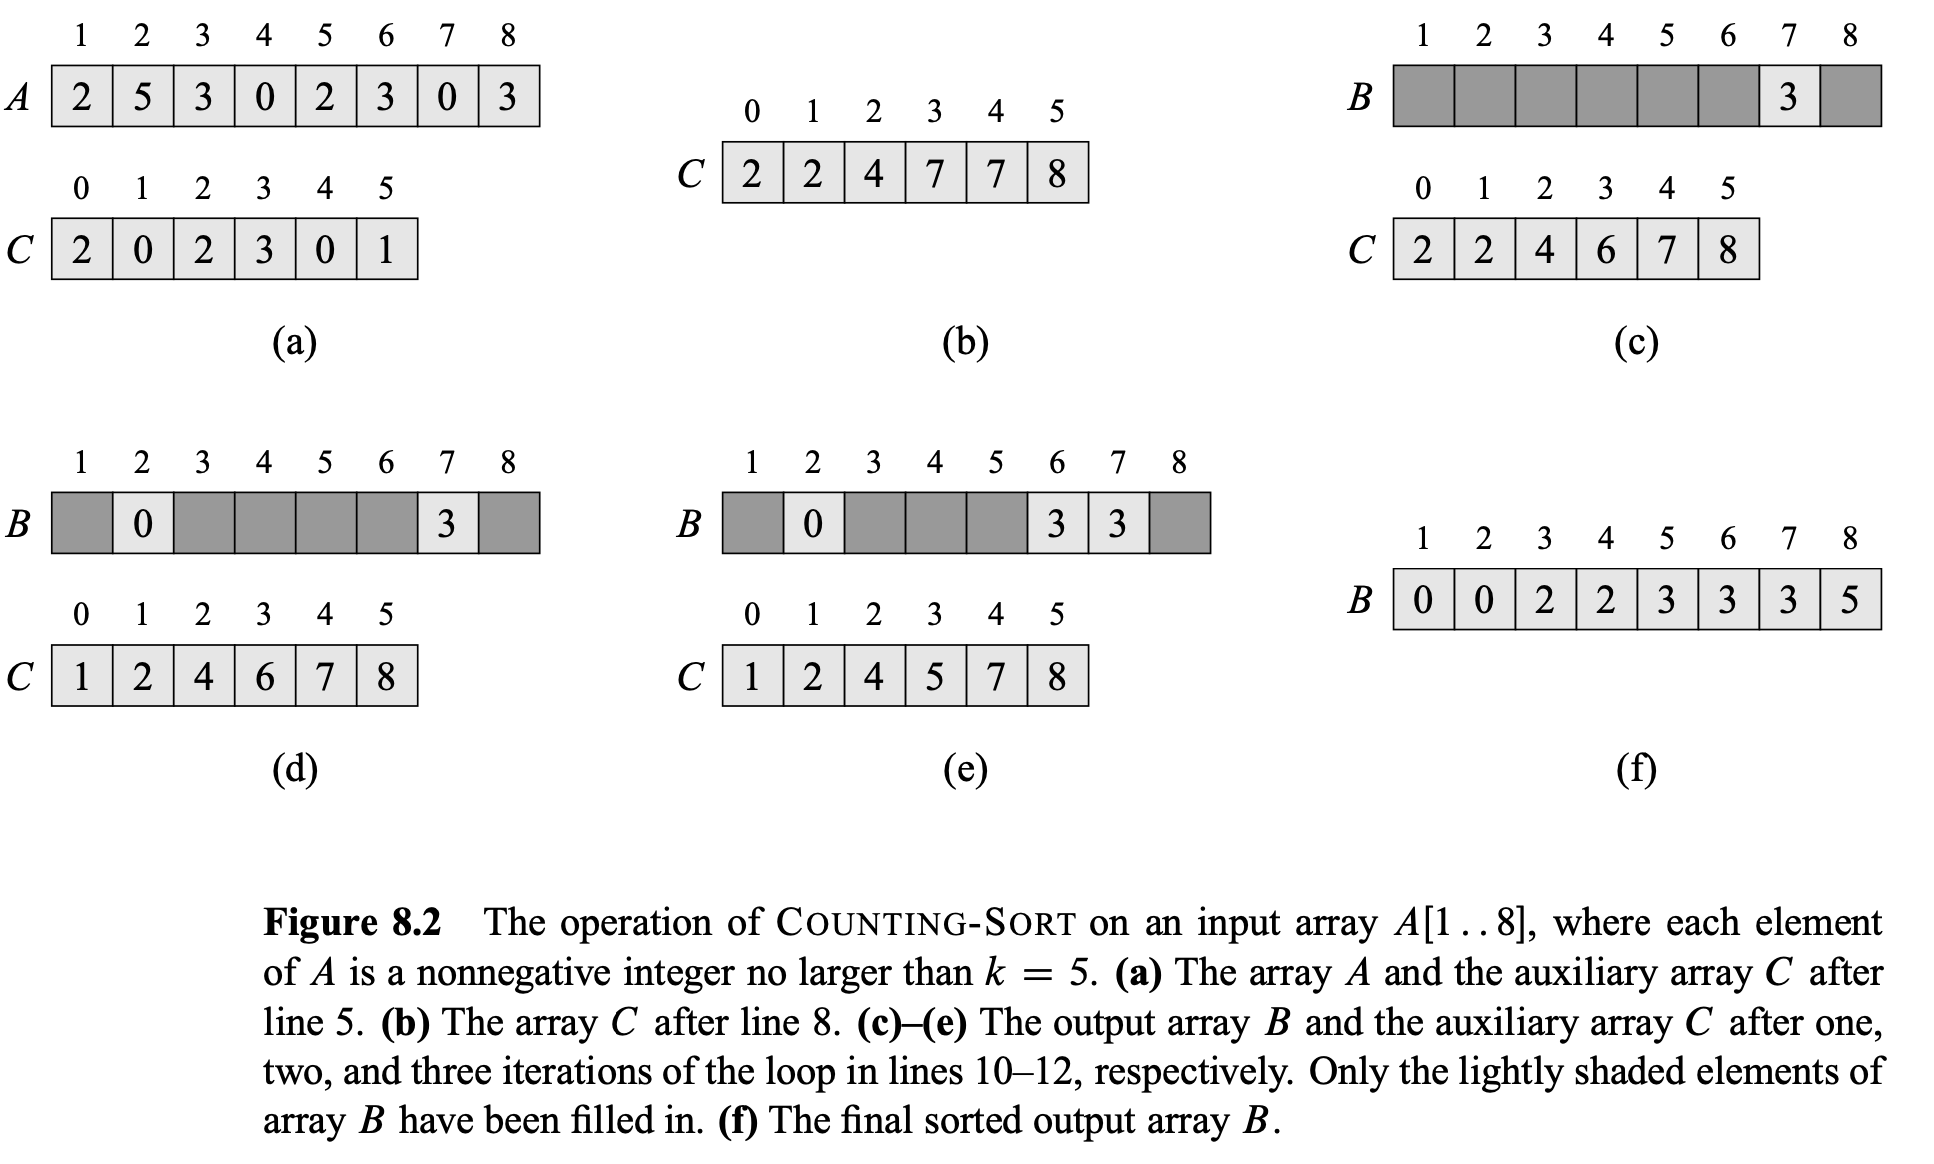
\includegraphics[scale=0.43]{images/06-counting-eg.png}
    \end{center}
    

    \section{Radix Sort}

    {\bf Radix Sort} is quite interesting. With the help of a {\it stable 
    sort}, where Counting Sort will be a good choice, it sorts the array 
    on one digit, each time, from {\bf least-significant bit}(LSB) to 
    {\bf most-significant bit}(MSB).

    Here is what Radix Sort does, on an input of array of $n$ items,
    each of them has $d$ digits, and digit $1$ is the right-most digit(LSB),
    digit $d$ is the left-most digit(MSB).

    \begin{algorithm*}
        \caption{Radix-Sort($A,d$)}
        \For{$i\lar 1$ to $d$}{
            use {\bf counting sort} to sort array $A$ on digit $i$
        }
    \end{algorithm*}
    Here is an example of what Radix Sort does on each step:
    \begin{center}
        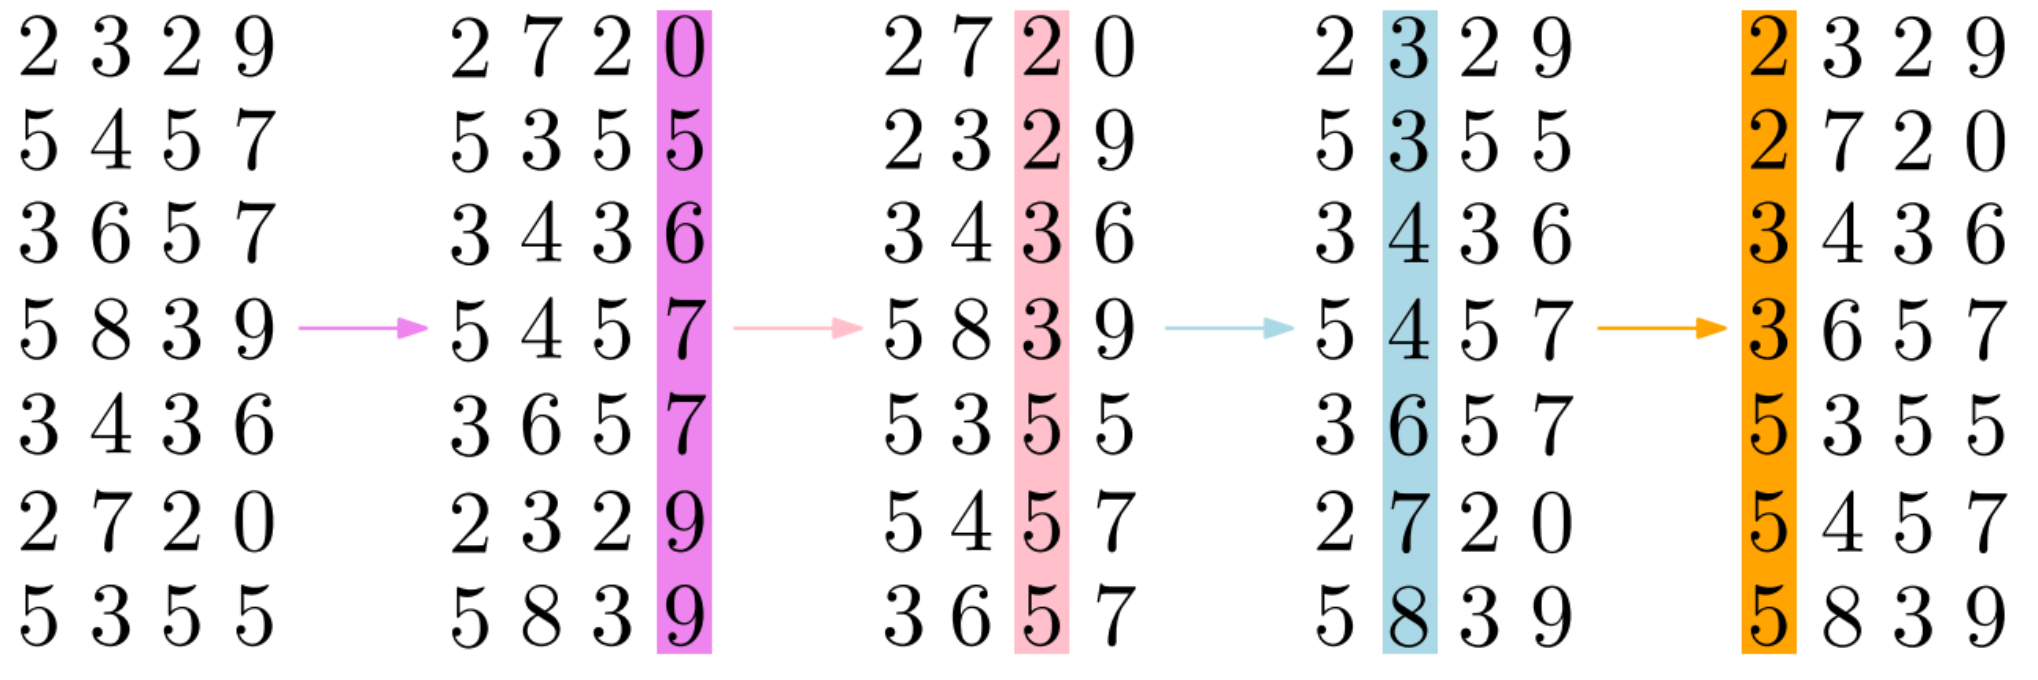
\includegraphics[scale=0.4]{images/06-radix-eg.png}
    \end{center}
    Since here we are focusing on decimal numbers, so for counting sort, 
    $k=10$(each digit is in $\{0,1,\cdots, k-1\}$). It is not necessary that 
    we sort it on decimal numbers, actually each digit can be of any range,
    maybe hexadecimal, binary, etc, since all of them work fine with 
    Counting Sort.

    We prove the correctness of Radix Sort by induction.
    \begin{proof}
        Assume that the numbers are already sorted by their low-order $i-1$ digits.
        (that is, we've already use radix sort on digit $1\cdots i-1$)

        Now assume sorting on digit $i$. 
        \begin{itemize}
            \item Two numbers that differ on digit $i$ will be correctly sorted 
            by their $i-$th digit, 
            \item Two numbers that we same digit $i$ will be put in the same order 
            in output as they were in input, since we are using a stable sort,
            (Counting Sort, usually)
        \end{itemize}
        Therefore, they are correctly sorted by their $i-$th digits.
    \end{proof}

    The running time of Radix Sort is depends on three variables: $n$, the size of input, 
    $k$, the numbers of values that each digit can take, and $d$, number of digits 
    in each item.

    We know Counting Sort takes $\Theta(n+k)$ time, and for Radix Sort, we run 
    Counting Sort for $d$ times, its running time should be $\Theta(d(n+k))$.

    If you remember what we said above, it is not necessary that we represent each 
    item in decimal numbers. If we are given $n$ hexadecimal numbers, $k$ changes 
    from $10$ to $16$, but $d$ will become smaller. On the contrary, if we are given 
    $n$ binary numbers, $k$ will be only 2, but $d$ will become larger.


    \section{Sort Review}

    For now, you've seen those sorting algorithms.
    \begin{center}
        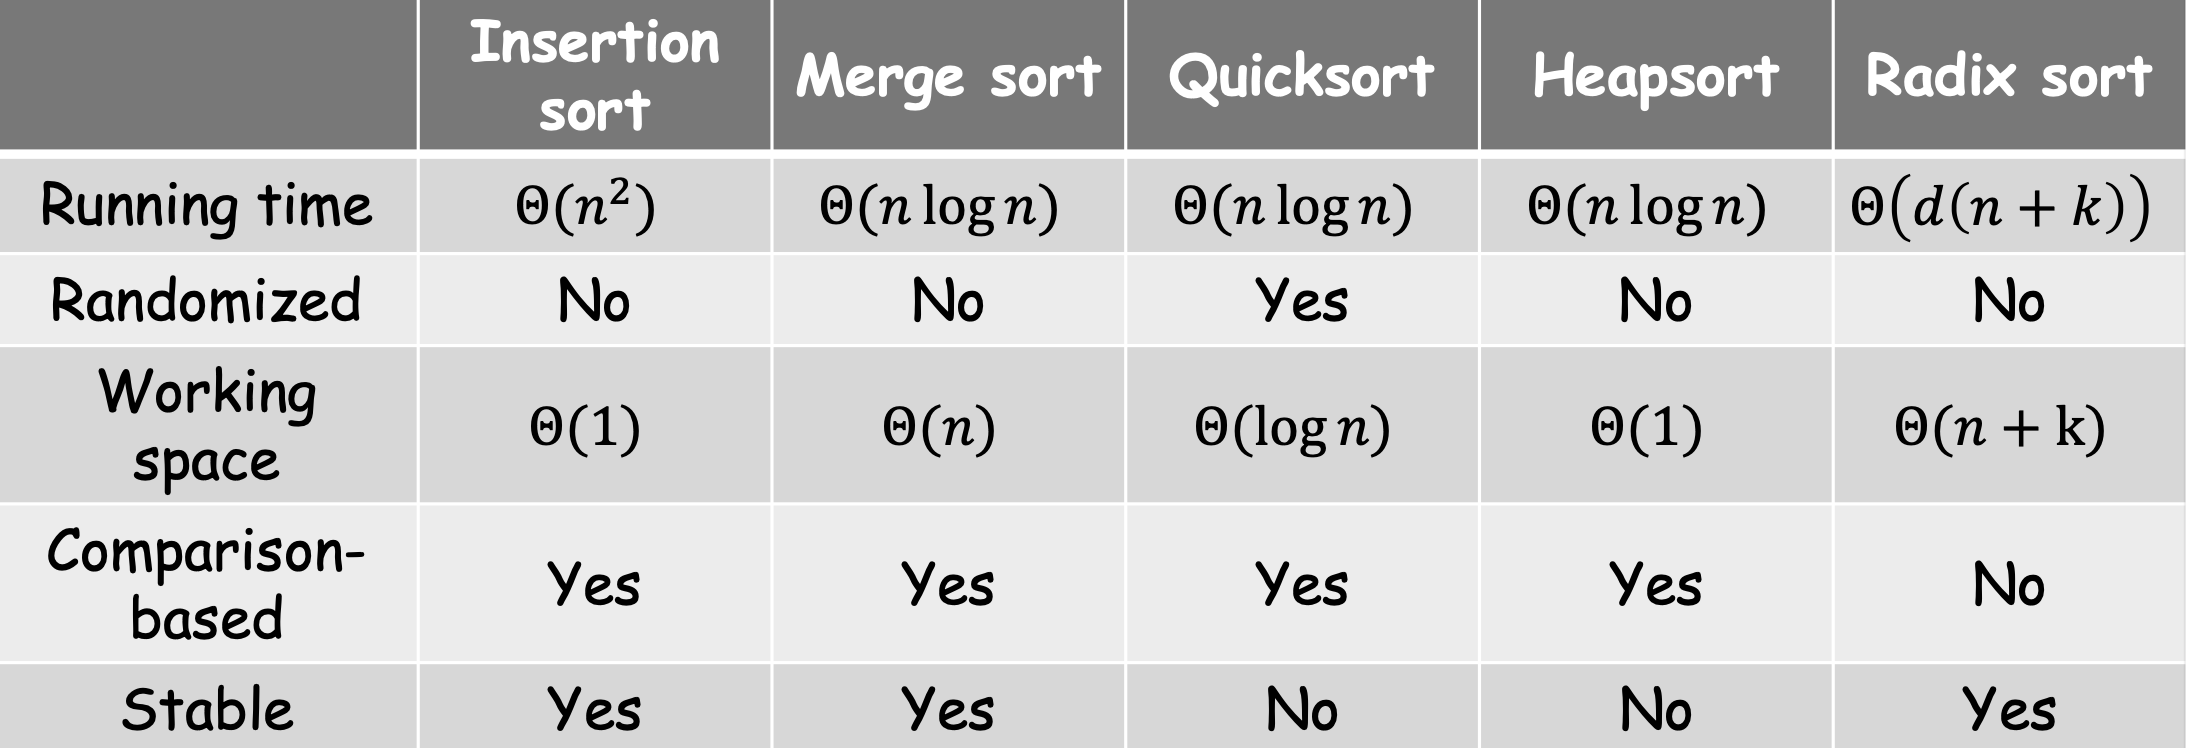
\includegraphics[scale=0.4]{images/06-sort-review.png}
    \end{center}

    
\end{spacing}





\part{Advanced Design Techniques}

\chapter{Greedy}

\begin{spacing}{1.3}

    \section{Introduction}

    Let's first define(informally) what is a {\bf Greedy Algorithm}. Consider for a problem 
    that requires us to find some kinds of {\it optimal solutions}, and to find it, 
    we always makes the choice that {\it looks best at current moment}, and choose it as 
    a part of our final solution.

    This idea may sound natural, simple, and even runs efficiently. Indeed it is, however, 
    one may alert that this strategy doesn't always give us the optimal solution 
    {\it of the whole problem}(we only make optimal choice at each step, we cannot guarantee 
    the solution is still optimal after all steps). We will see some problems that greedy 
    algorithm fails to find optimal.

    As you can see, greedy algorithm is really easy, while the hardest part is how to formally
    {\it prove} it. You must convince other people that your greedy algorithm is able to 
    find {\it global optimal solution} by simply grab {\it optimal solution at each step}.
    We will cover three different kinds of problems(except for Huffman Coding, which is a special one) 
    where greedy algorithm performs well, and the first two have similar proof of correctness,
    while the third one has a totally different proof.
    (You may be required to redo the proof or adapt the proof to another similar 
    problem in homework/exam)


    \section{Interval Scheduling}

    {\bf Problem:} Given $n$ jobs, where job $j$ starts at time $s_j$ and finishes at $f_j$.
    We say two jobs $i$ and $j$ are {\it compatible} or {\it not overlap} if their time intervals 
    $(s_i, f_i)\cap (s_j, f_j) = \emptyset$. Our goal is to find the maximum-size subset
    of {\it mutually compatible} jobs.
    \begin{center}
        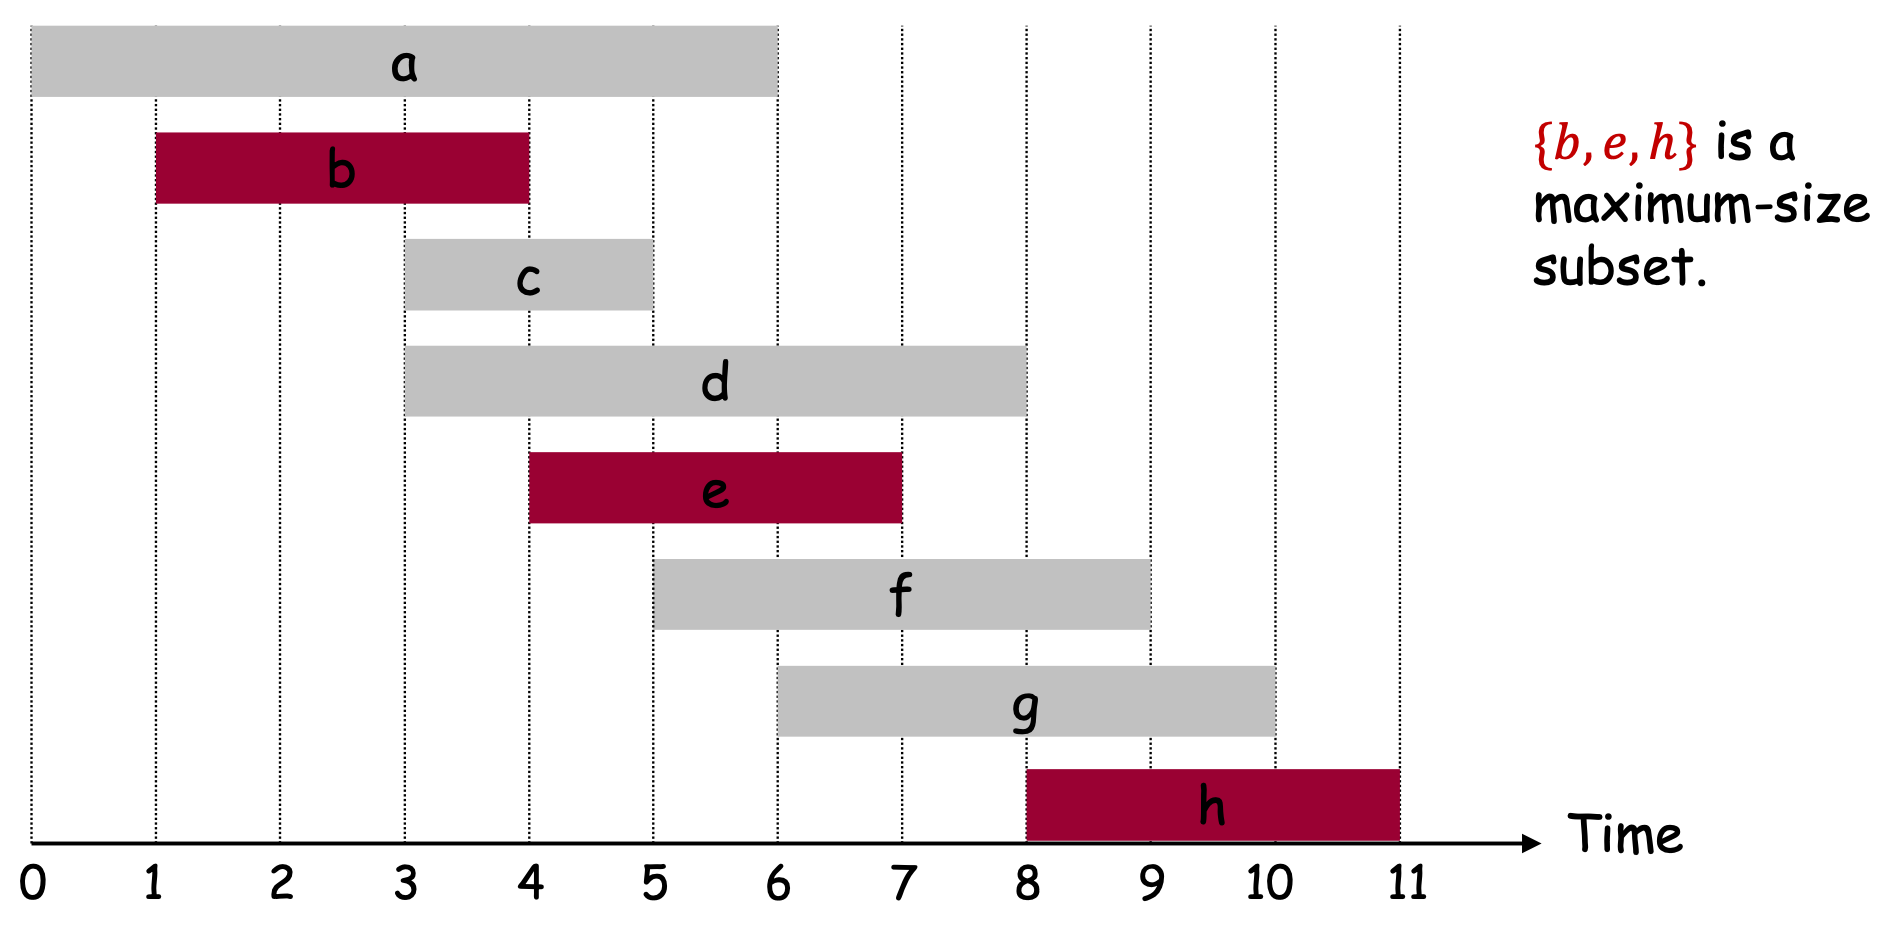
\includegraphics[scale=0.35]{images/07-interval-example.png}
    \end{center}
    In the example above, $\{b,e,h\}$ is a maximum-size subset, since you cannot find 
    a subset of size more than 4 and the jobs in that subset are mutually compatible.

    We consider to solve this problem by greedy, that is, given some jobs, we need 
    to make the best choice at current timestamp, that could make the size of subset maximized.
    So how can we maximized it? Consider choosing a job if it is compatible with all previous ones 
    that we've already taken, and not choosing it otherwise. In this way we achieve what we said that 
    ``make the best current choice''.

    However, you may easily find a counterexample, like if we first encounter a job that overlap 
    with all other jobs, then we can choose at most one job using the strategy above. So to ensure 
    its correctness, we need to first {\it consider jobs in some order}, and then use the above method.

    This order can be hard to decide, and one may think of sort jobs by:
    \begin{enumerate}
        \item increasing order of {\it start time} $s_j$,
        \item increasing order of {\it interval length} $f_j-s_j$,
        \item increasing order of {\it fewest conflicts} of each job,
        \item increasing order of {\it finish time} $f_j$.
    \end{enumerate}

    Unfortunately, we can find(not difficult) counterexamples for first three orders:
    \begin{center}
        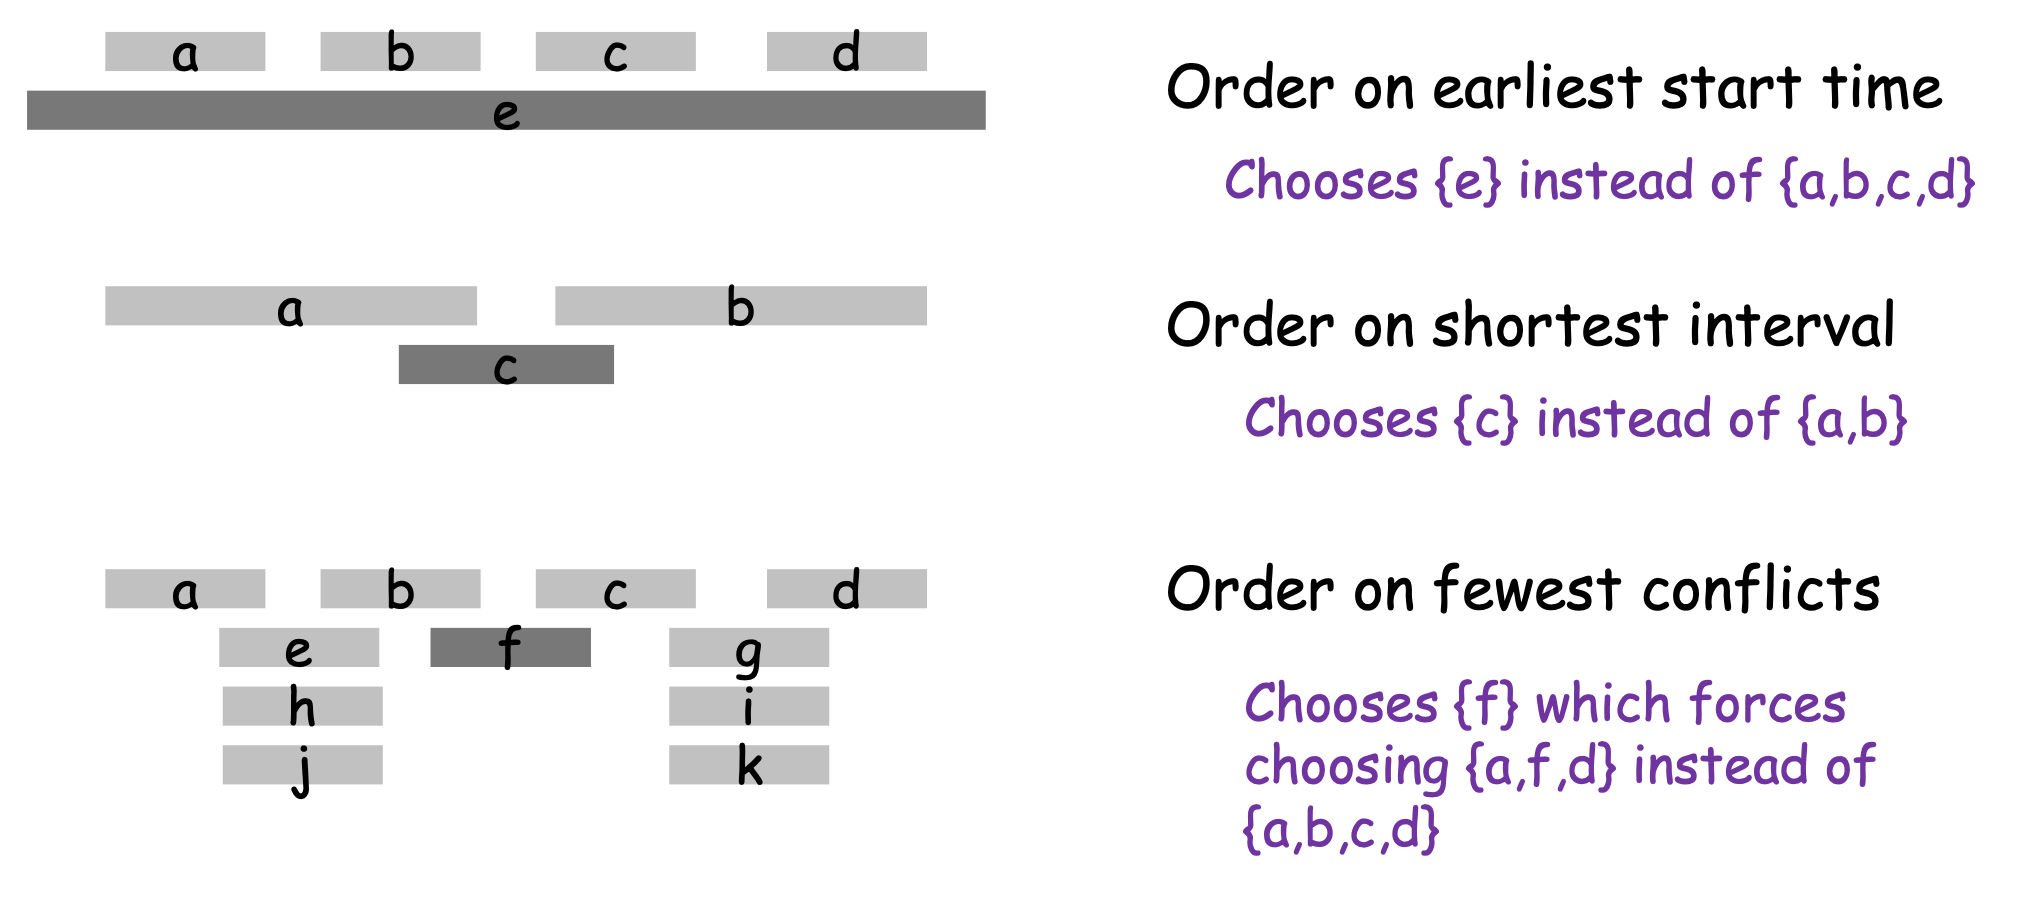
\includegraphics[scale=0.35]{images/07-interval-countereg.png}
    \end{center}

    The fourth order, i.e., sort jobs by {\it finish time}, can actually guarantee the greedy 
    algorithm to be optimal. This is not easy to find out, but the intuition is that 
    we can leave {\it maximum time} for scheduling {\it the rest of jobs}.

    You may want to review this image:
    \begin{center}
        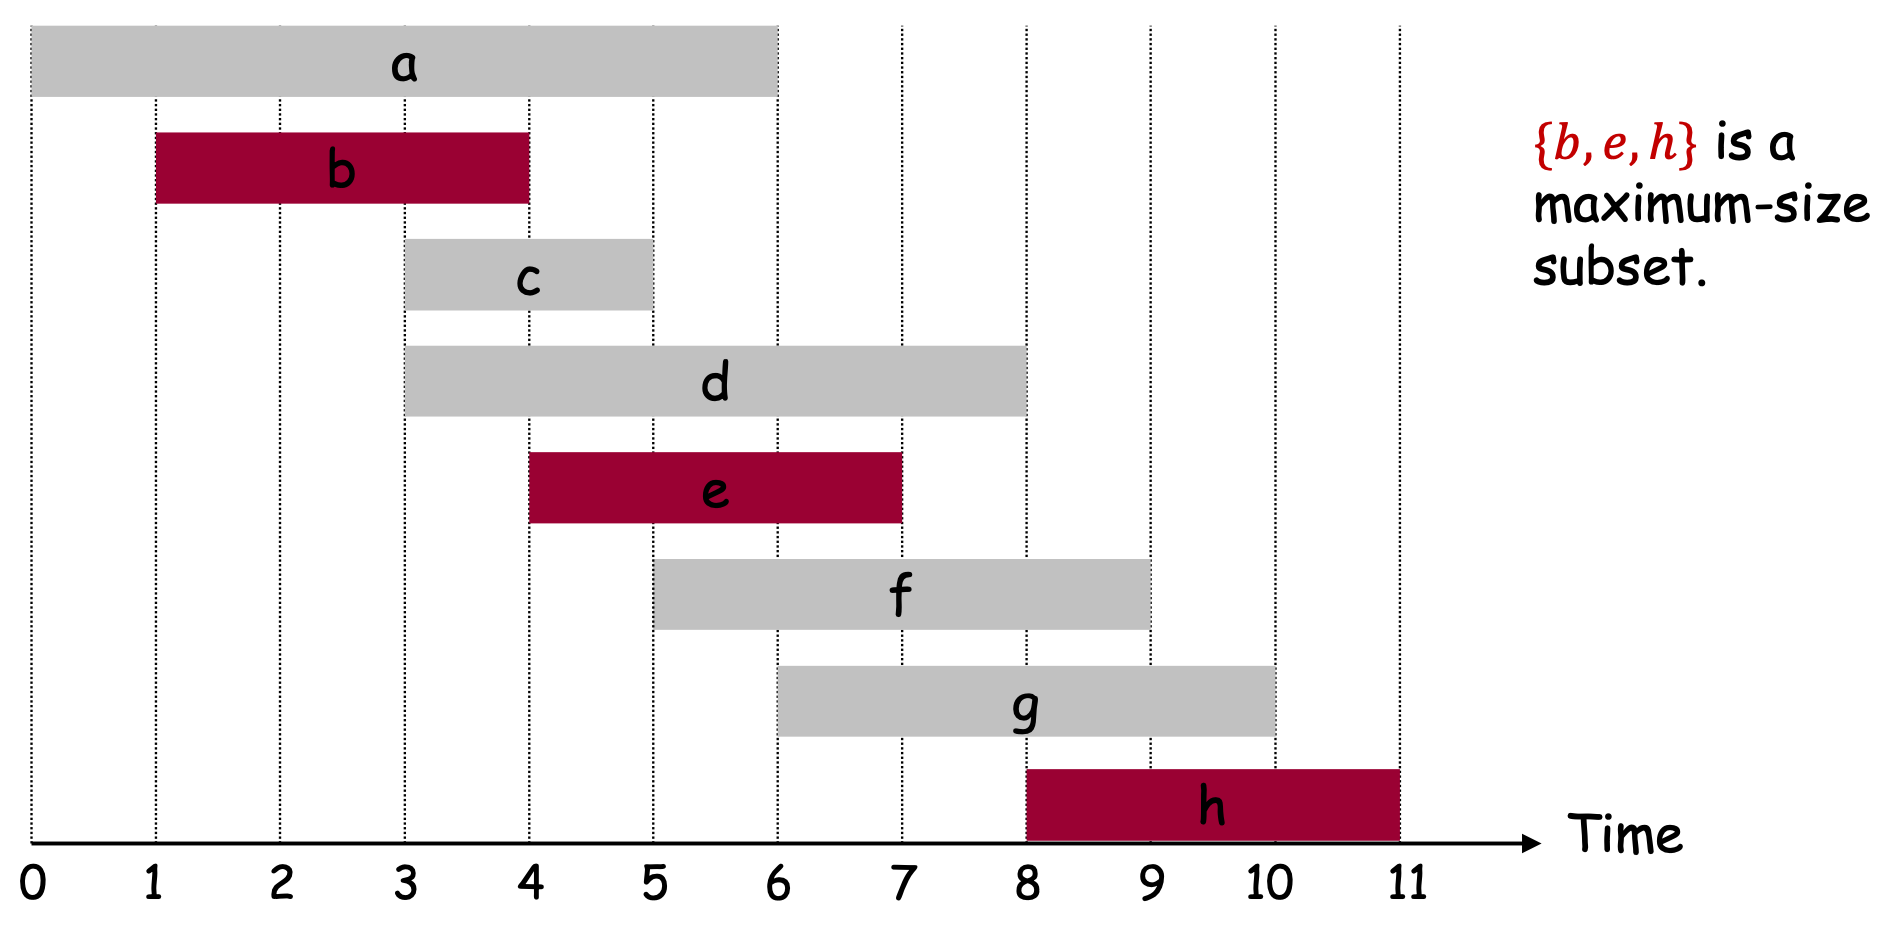
\includegraphics[scale=0.35]{images/07-interval-example.png}
    \end{center}
    We first give the code that implements this algorithm, and then formally prove it.
    
    \begin{algorithm*}
        \caption{Interval-Schedule($(s_1,f_1), \cdots, (s_n, f_n)$)}
        Sort jobs by finish time so that $f_1\le f_2\le \cdots \le f_n$

        $A\lar \emptyset$ \qquad \tcp{$A$ is the set to store the subset we found}

        $last \lar 0$   \qquad \tcp{$last$ records the {\it finish time} of last job we've chosen}

        \For{$j\lar 1$ to $n$}{
            \tcp{If job $j$ is compatiable with previous jobs, i.e., starts no earliear than 
            the finish time of last job we've chosen}
            \If{$s_j\ge last$}{
                $A\lar A\cup \{j\}$\qquad \tcp{Add job $j$ into our set}

                $last \lar f_j$ \qquad \tcp{Update $last$}
            }
        }
        return $A$
    \end{algorithm*}

    The running time of this algorithm is dominated by sorting process, which causes $\Theta(n\log n)$.

    Now let's prove the correctness of this algorithm, i.e., {\it the greedy algorithm is optimal}.

    Assume the set of jobs we get from greedy algorithm is different from an optimal set.
    Let $i_1,i_2,\cdots, i_k$ be the set of jobs found by greedy algorithm, while 
    $j_1,j_2,\cdots,j_m$ be the set of jobs in optimal solution. Our basic idea is to 
    {\it modify} optimal solution into the same as our greedy solution, while at the same time 
    {\it ensure the solution is still optimal after modification.}

    We start by finding largest possible value of $r$ such that $i_1=j_1, i_2=j_2, \cdots, i_r=j_r$,
    that is, find the last job that are the same in both sets. Thus, $i_{r+1}\ne j_{r+1}$.

    Notice in our greedy algorithm, we sort jobs by increasing of finish time, so if $i_{r+1}\ne j_{r+1}$,
    there must be job $i_{r+1}$ finishes no later than $j_{r+1}$, i.e., $f_{i_{r+1}}\le f_{j_{r+1}}$.
    \begin{center}
        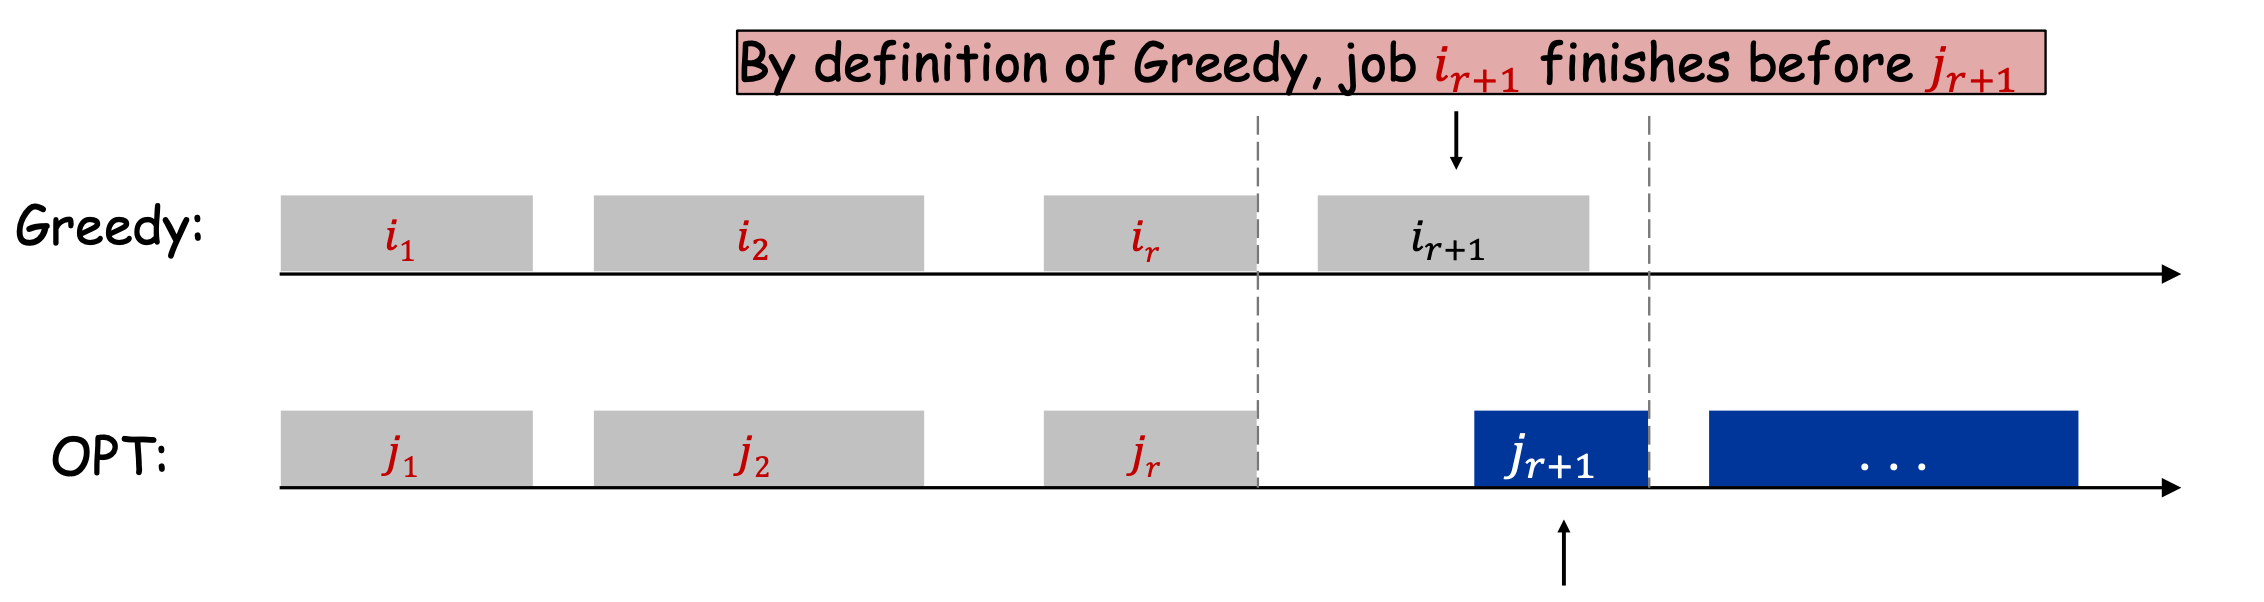
\includegraphics[scale=0.35]{images/07-interval-proof.png}
    \end{center}
    Then, we try to modify optimal solution, say, create $OPT^\star$ from $OPT$ by just replacing 
    $j_{r+1}$ with $i_{r+1}$. Notice now $OPT^\star$ is still a legal solution, the jobs are
    still mutually compatible, and $OPT^\star$ has the same size as $OPT$, so $OPT^\star$ is 
    also an optimal solution!

    Let's do this process again, until the optimal solution is the same as greedy.
    A minor problem is that they may not have the same size, i.e., $k\ne m$. 
    If this happens, the only possible is $k<m$, since $m$ is the size of optimal solution, 
    it must be the largest! However, $k<m$ is also impossible, since after replacing 
    all jobs using above method, $i_1=j_1, i_2=j_2,\cdots, i_k=j_k$. If there is 
    still jobs in optimal solution, say $j_{k+1}$, that is compatible with all previous 
    jobs, then our greedy algorithm must would have chosen that(this holds immediately 
    from our algorithm). So there must be $k=m$.


    \vspace{0.5in}
    \section{Knapsack}

    {\bf Problem:} Given $n$ items, where item $i$ has weight $w_i$ and value $v_i$.
    You now only has a knapsack that can holds weight at most $W$, you want to fill 
    your knapsack with as much {\it value} as possible. Notice in this problem an item 
    can be {\it partially used}, like each item is some liquid.

    The idea is quite simple: since we can partially use an item, we just first choose 
    items with largest ``value-weight ratio'', i.e., largest $\dfrac{v_i}{w_i}$.
    If the bag is full, we stop choosing, otherwise, we repeat the process 
    on remaining items.

    \begin{algorithm*}
        \caption{Fractional-Knapsack($w_1, v_1, w_2, v_2, \cdots, w_n, v_n, W$)}
        Sort items so that $\dfrac{v_1}{w_1}\ge \dfrac{v_2}{w_2}\ge \cdots \ge \dfrac{v_n}{w_n}$

        $w\lar W$\qquad \tcp{$w$ records how many {\it more} weight can the knapsack hold}

        \For{$i\lar 1$ to $n$}{
            \tcp{If $w_i\le w$, we can choose whole item, otherwise, we can only choose partial}
            \eIf{$w_i\le w$}{
                $x_i\lar 1$\qquad \tcp{$x_i$ records how much of the item is chosen, 1 means whole}

                $w\lar w-w_i$\qquad \tcp{update remaining capacity of the knapsack}
            }{
                $x_i\lar w/w_i$\qquad \tcp{choose partial}

                return \qquad \tcp{No need to update $w$, since we are already done}
            }
        }
        return
    \end{algorithm*}

    Again, its running time depends on the sorting process, which is $\Theta(n\log n)$.

    To prove the correctness of this greedy algorithm, we can assume $\disp \sum_{i=1}^n w_i\ge W$, 
    i.e., the knapsack is fully packed. Otherwise, the algorithm just takes all items thus 
    is trivially optimal.

    For the following proof, we assume the items are already {\it sorted by 
    } ``value-weight ratio''.
    
    We will use the technique in last example, let the greedy solution be 
    $G=(x_1,x_2,\cdots, x_k, 0, \cdots, 0)$, where for $i<k, x_i=1$, since we fully take those items,
    and for $k$-th item, $0\le x_k\le 1$, since we may or may not fully take it, and 
    for $i>k, x_i=0$, since they are not so ``valuable'' and we didn't take it.
    Also consider some optimal solution $OPT=(y_1,y_2,\cdots, y_n)$. Note that since 
    both of them must fully pack the knapsack, there must be:
    $$\sum_{i=1}^k x_i w_i=\sum_{i=1}^n y_i w_i = W$$

    Again, we find the first item $i$ where $G$ and $OPT$ differ:
    
    \begin{tabular}{ccccccccccccc}
        $G$ & $=$ & $x_1$ & $x_2$ & $x_3$ & $\cdots$ & $x_{i-1}$ & {\blue $x_i$} & $\cdots$ & $x_k$ & $\cdots$ & 0 & 0\\
        $OPT$ & $=$ & $x_1$ & $x_2$ & $x_3$ & $\cdots$ & $x_{i-1}$ & {\blue $y_i$} & $\cdots$ & $y_k$ & $\cdots$ & $y_{n-1}$ & $y_n$\\
    \end{tabular}
   
    Since our algorithm is greedy, it will take item $i$ as much as possible, 
    so there must be $x_i>y_i$. We let $\Delta x=x_i-y_i>0$.

    We can then modify the $OPT$ as follows:
    \begin{itemize}
        \item change $y_i$ to $x_i$, i.e., take as much as what we've taken in greedy 
        \item remove some items in $i+1,\cdots,n$, such that their total weights equal 
        to $\Delta x$.
        \item What we have done up to now is that we take more item $i$ while 
        throw away equal weights of $i+1,\cdots,n$ items.
        \item Since those items are sorted by ``value-weight ratio'', as stated before, 
        the value of $OPT$ after modification {\it must have not decreased}.(think why)
        \item Since the value of $OPT$ must have already been the largest before modification, 
        so the value of $OPT$ must not change. 
        \item So the new solution $OPT^\star$ must still be an optimal solution.
    \end{itemize}

    In the same way, we repeat this process, and will eventually convert $OPT$ to $G$.

    Hence our greedy algorithm yields an optimal solution, the correctness is proved.

    \vspace{0.3in}
    One thing worths mentioning is that if this problem is modified into ``items 
    cannot be partially used'', i.e., you can only either choose the item, or 
    not choose the item(also known as ``0/1 Knapsack Problem''), then there is no 
    greedy algorithm that yields optimal solution. We will come back to this in 
    Dynamic Programming.


    \section{Interval Partitioning}

    {\bf Problem:} There are $n$ lectures, where lecture $j$ starts at 
    time $s_j$ and finishes at time $f_j$. Our goal is to find the {\it minimum 
    number of classrooms} to schedule ALL lectures so that no two occurs at the 
    same time in the same room.

    For example, the below schedule, which uses 3 classrooms, is the optimal 
    solution for given lectures.
    \begin{center}
        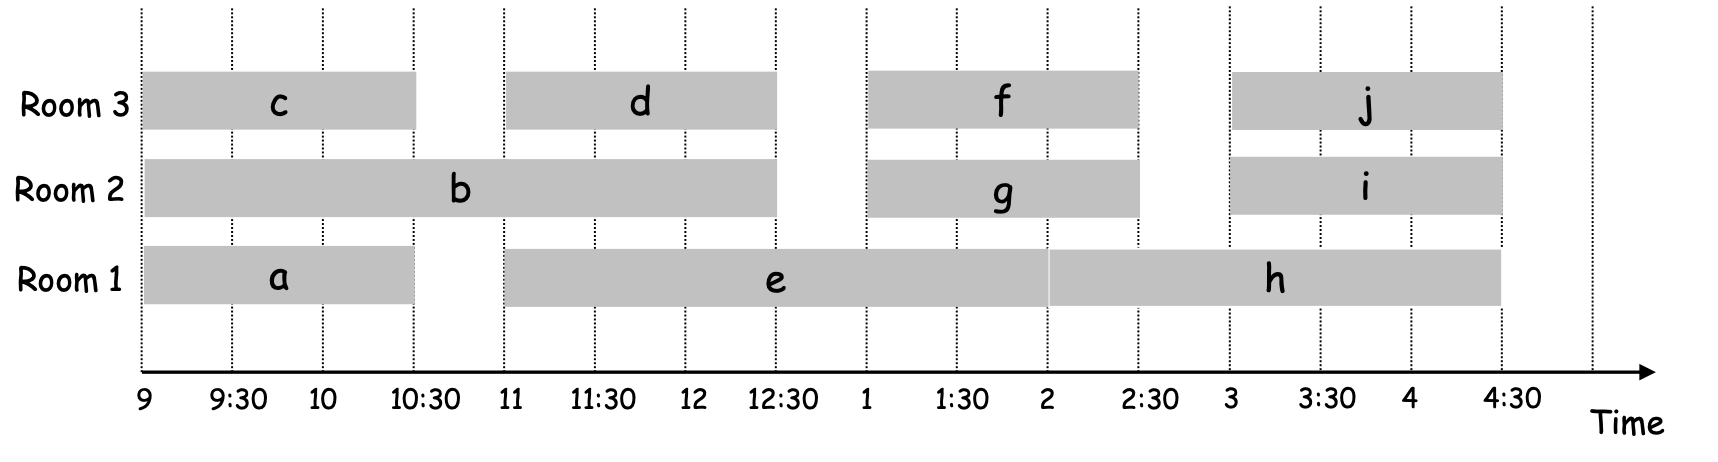
\includegraphics[scale=0.5]{images/07-interval-part-demo.png}
    \end{center}

    For this problem, we sort lectures in increasing order of {\it start time}, 
    and assign each lecture to any compatible classroom. That is, 
    for each lecture $j$, if there is an existing classroom $k$ such that 
    $k$ is empty during time interval $(s_j, f_j)$, then we assign lecture $j$
    to classroom $k$.

    Otherwise, if all existing classrooms are incompatible with the lecture, 
    we allocate it to a new classroom.

    The algorithm is shown below:

    \begin{algorithm*}[htbp]
        \caption{Interval-Partition($(s_1,f_1)\cdots (s_n, f_n)$)}
        Sort intervals by starting time so that $s_1\le s_2\le \cdots \le s_n$

        $d\lar 0$\quad \tcp{$d$ records \# of classrooms used so far}

        \For{$j\lar 1$ to $n$}{
            \eIf{lecture $j$ is compatible with some classroom $k$}{
                schedule lecture $j$ in classroom $k$
            }{
                allocate a new classroom numbered $d+1$

                schedule lecture $j$ in classroom $d+1$

                $d\lar d+1$
            }
        }
        return $d$
    \end{algorithm*}

    (Before we prove this is optimal, you should convince yourself that sorting by 
    finish time does not yield optimal.)

    Firstly, we define ``depth'' of a set of lectures(or generally, a set of open intervals).

    \begin{definition}
        The {\bf depth} of a set of open intervals is the maximum number that 
        exist at any instant of time.
    \end{definition}
    Intuitively, at each second of the day, you record how many {\it simultaneous classes}
    are being taught at that second, and the ``depth'' is the max number of all 
    those numbers you have recorded.

    Unsurprisingly, the minimum number of classrooms required must be $\ge $ depth.
    For example, back to our example at the beginning, the {\bf depth of the lectures} 
    is 3, so we expect we should at least use 3 classrooms. Well, interestingly, 
    the schedule we give below uses just 3 classrooms. Thus, we are sure that this schedule
    is optimal.
    \begin{center}
        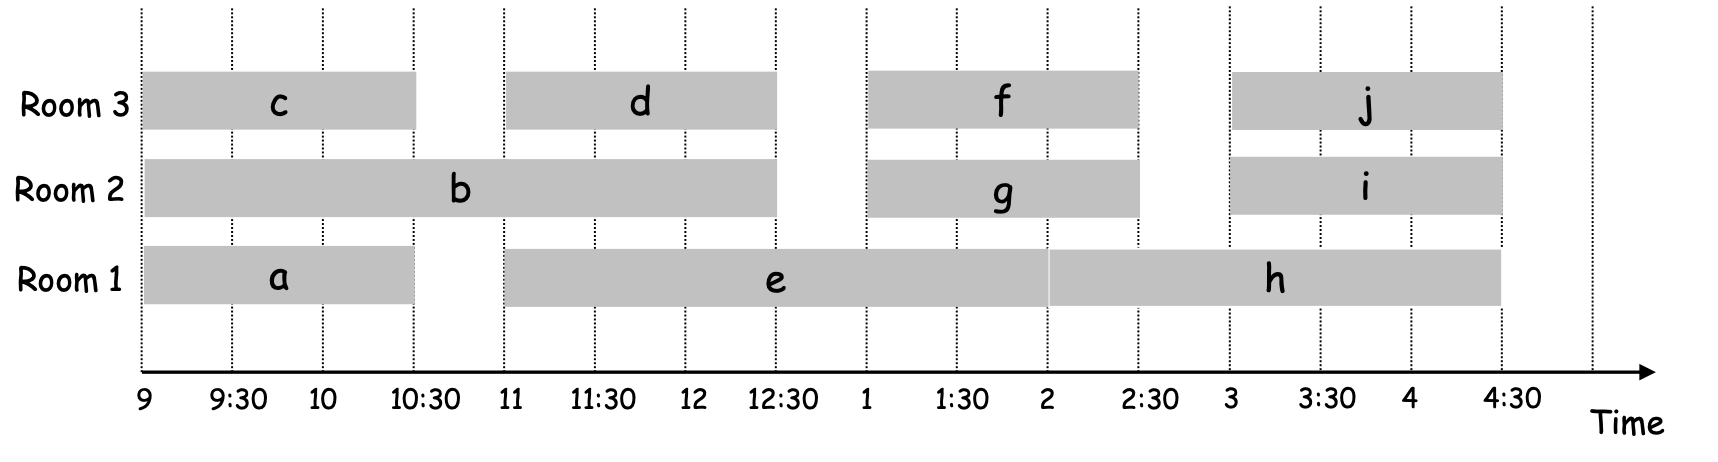
\includegraphics[scale=0.5]{images/07-interval-part-demo.png}
    \end{center}

    Now, to prove our greedy algorithm is optimal, we only need to show 
    the \# classrooms used by our greedy algorithm {\it equals to} ``depth''.

    \begin{theorem}
        The number of classrooms used by greedy, say $d$, is no more than 
        the {\bf depth} of the set of lectures, i.e., $${\rm depth} \ge d$$
    \end{theorem}

    \begin{proof}
        Let $d$ be the number of classrooms used by greedy.
        \begin{itemize}
            \item Classroom $d$ is opened because we need to schedule a lecture $j$, 
            while $j$ is incompatible with all $d-1$ other classrooms.
            \item Since we sorted by start time, all these incompatibilities are caused 
            by lectures that are {\it start no later than $s_j$}, and 
            {\it finish later than $s_j$}.
            \item Thus, there $\exists \epsilon > 0$, where at time $s_j+\epsilon$,
            all $d$ lectures(the $d-1$ incompatible ones and lecture $j$) are overlapping. 
            \item Therefore, there are at least $d$ lectures at time $s_j+\epsilon$
            \item $\Rightarrow $ depth $\ge d$ 
        \end{itemize}
        Since the number of classrooms used by greedy, $d$, is $\le $ depth,
        our greedy is optimal.
    \end{proof}

    Now back to our algorithm, let's analyze its running time. (see codes below)

    \begin{algorithm*}[htbp]
        \caption{Interval-Partition($(s_1,f_1)\cdots (s_n, f_n)$)}
        Sort intervals by starting time so that $s_1\le s_2\le \cdots \le s_n$

        $d\lar 0$\quad \tcp{$d$ records \# of classrooms used so far}

        \For{$j\lar 1$ to $n$}{
            \eIf{lecture $j$ is compatible with some classroom $k$ \qquad (*)}{
                schedule lecture $j$ in classroom $k$ \qquad (**)
            }{
                allocate a new classroom numbered $d+1$

                schedule lecture $j$ in classroom $d+1$ \qquad (***)

                $d\lar d+1$
            }
        }
        return $d$
    \end{algorithm*}

    To achieve line (*), we need to maintain for each classroom, the finishing time 
    of the last lecture placed in that classroom. So at line (*), we compare 
    $s_j$ with those finishing times. If $s_j\ge $ any one of those finishing time,
    we can schedule lecture $j$ into that classroom.

    Therefore, line (*) uses $O(n)$ time to check, this algorithm runs in $O(n^2)$ time.

    However, it is possible to improve it. Consider if the finishing time of 
    classrooms are
    $$[3, 5, 6, 4, 9],$$
    and now we have a lecture $j$ such that $s_j=2$. Notice that since $s_j$ is 
    incompatible with the first classroom, which ends at 3, then we don't bother 
    to check all remaining ones! 3 is the {\it earliest finishing time} among all 
    classrooms, if $j$ is not compatible with that one, it cannot be compatible
    with any other classrooms. On the contrary, if we have a lecture $k$ such that 
    $s_k=3$, then we also only need to check the first classroom, which ends at 3, 
    and they are compatible! And we still need to check others.

    Hence, we could maintain the classrooms in a {\bf min priority queue}, 
    using the finishing time of the last class in that room as the key value.
    To implement (*), we do {\bf extract-min} to get the {\it earliest finishing
    time} among all classrooms $f_{min}$, and check whether $f_{min}\le s_j$.
    If $f_{min}> s_j$, we need a new classroom.

    For line (**), we just need to add the new finishing time $f_j$ to 
    priority queue.

    For line (***), we {\it re-insert} $f_{min}$ back to priority queue,
    (since we extracted it before) AND 
    insert the new finishing time $f_j$ into priority queue.

    Under this implementation, all (*), (**), and (***) lines are $O(\log n)$
    jobs, so the algorithm runs in $O(n\log n)$ time.



    \section{Huffman Coding}





    



    \newpage
    \section{Exercises}

    {\it Those problems are extracted from COMP3711 past paper or previous assignments. 
    Please find solution after the problems.}

    1. (2019Spring, Midterm, 3, 18pts) {\bf Interval Scheduling}
    
    In this problem you will describe and explain the correctness of the interval scheduling algorithm that was taught in class.
    
    {\it The Interval Scheduling Problem}: Suppose that you are given $n$ intervals $I_{1}, I_{2}, \ldots, I_{n-1}, I_{n}$ that are sorted from left to right according to some criterion. For $1 \leq i \leq n$, the start and finish times of $I_{i}$ are denoted by $s_{i}$ and $f_{i}$, respectively. Two intervals $I_{i}$ and $I_{j}$ are compatible if their interior do not overlap, i.e., $s_{i} \geq f_{j}$ or $s_{j} \geq f_{i}$. The interval scheduling problem is to select a subset of mutually compatible intervals that has the maximum size.
    
    {\it The Greedy Algorithm}: The following pseudocode describes a greedy algorithm for the interval scheduling problem.
    
    1. $A \leftarrow\left\{I_{1}\right\}$;\\
    2. for $j=2$ to $n$\\
    3. \quad if $I_{j}$ is compatible with the intervals in $A$\\
    4. \quad \quad \quad $A \leftarrow A \cup\left\{I_{j}\right\} ; \quad /^{*}$ add $I_{j}$ to the set $A * /$\\
    5. output the set $A$

    We have not specified HOW the intervals are sorted. Consider the following two ways of sorting:
    
    \noindent (a) By increasing starting time, i.e., $s_{1} \leq s_{2} \leq \cdots \leq s_{n}$.\\
    (b) By increasing finishing time, i.e., $f_{1} \leq f_{2} \leq \cdots \leq f_{n}$.
    
    Answer the following question separately for each of the two sorting orders in (a) and (b) above.
    
    {\bf Will the greedy algorithm return a subset of mutually compatible intervals that has the maximum size? Explain.}
    
    If the answer is yes, provide a formal proof of correctness.
    
    If the answer is no, provide a counterexample. Your counterexample should specify a set of input intervals. You should state the subset returned by the greedy algorithm and explain why that subset is not a correct solution.


    \newpage
    2. (2021Spring, Final, 3, 14pts) {\bf Greedy Classroom Scheduling}

    Recall the greedy Interval Partitioning algorithm taught in class. The input was $n$ pairs of numbers $\left(s_{i}, f_{i}\right), i=1, \ldots, n$ for which $s_{i}<f_{i}$. Each pair represented a class: $s_{i}$ is class $i$ 's starting time, $f_{i}$ is its ending time. The goal was to find the minimum number of classrooms required to schedule all lectures so that no two occur at the same time in the same room. The algorithm taught in class is given below:
    
    1) Sort intervals by starting time so that $s_{1} \leq s_{2} \leq \cdots \leq s_{n}$\\
    2) $d \leftarrow 0 \quad$ \% \# classrooms used so far\\
    3) for $j \leftarrow 1$ to $n$\\
    4) \quad if lecture $j$ is compatible with some classroom $k$ then $\left(^{*}\right)$\\
    5) \quad \qquad schedule lecture $j$ in classroom $k\left(^{* *}\right)$\\
    6) \quad else\\
    7) \quad \qquad allocate a new classroom $d+1$\\
    8) \quad \qquad schedule lecture $j$ in classroom $d+1(* * *)$\\
    9) \quad \qquad $d \leftarrow d+1$
    
    (a) Prove that this algorithm gives the correct answer, i.e., it only opens the minimum number of classrooms necessary to schedule all classes.
    
    (b) Explain how to implement this algorithm in $O(n \log n)$ time. You need to say
    
    \qquad (i) what data structure you are using, and, in particular,

    \qquad (ii) how you use it to implement lines $4,5,8$ and

    \qquad (iii) why your algorithm requires $O(n \log n)$ time.

    \newpage
    3. (2020Spring, Final, 1, 15pts) {\bf Greedy Algorithms}

    Given two sequences of characters $X=\left(x_{1}, \ldots, x_{m}\right)$ and $Y=\left(y_{1}, \ldots, y_{n}\right)$ with $m \leq n$, design an $O(n)$ time algorithm that determines if $X$ is a subsequence of $Y$.
    
    Formally, $X$ is a subsequence of $Y$

    \qquad if there exists $1 \leq j_{1}<j_{2}<\cdots<j_{m} \leq n$ such that $x_{i}=y_{j_{i}}$.
    
    Example: let $Y=A B B C B D A B, X_{1}=B C B A$ and $X_{2}=B D B A$.
    
    Then $X_{1}$ IS a subsequence of $Y$, but $X_{2}$ is NOT a subsequence of $Y$.
    
    Your algorithm should return "YES" if $X$ is a subsequence of $Y$ and "NO" if $X$ is not a subsequence of $Y$.
    
    You can assume that your inputs are given as two character arrays $X[1 \ldots m]$ and $Y[1 \ldots n]$ storing $X$ and $Y$.
    
    (A) Using documented psuedocode, clearly describe how your algorithm works.
    
    (B) Formally prove that your algorithm is correct
    
    (C) Explain why it runs in $O(n)$ time.
    
    In part (B), put every argument on a separate line with space betwen the lines.
    
    Write your proof clearly. If you use induction in your proof, you must clearly state what your induction hypothesis is. If you prove by contradiction, clearly identify the statement that is being assumed wrong, etc.


    \newpage
    4. (2019Spring, Midterm, 2, 10pts) {\bf Huffman Coding}

    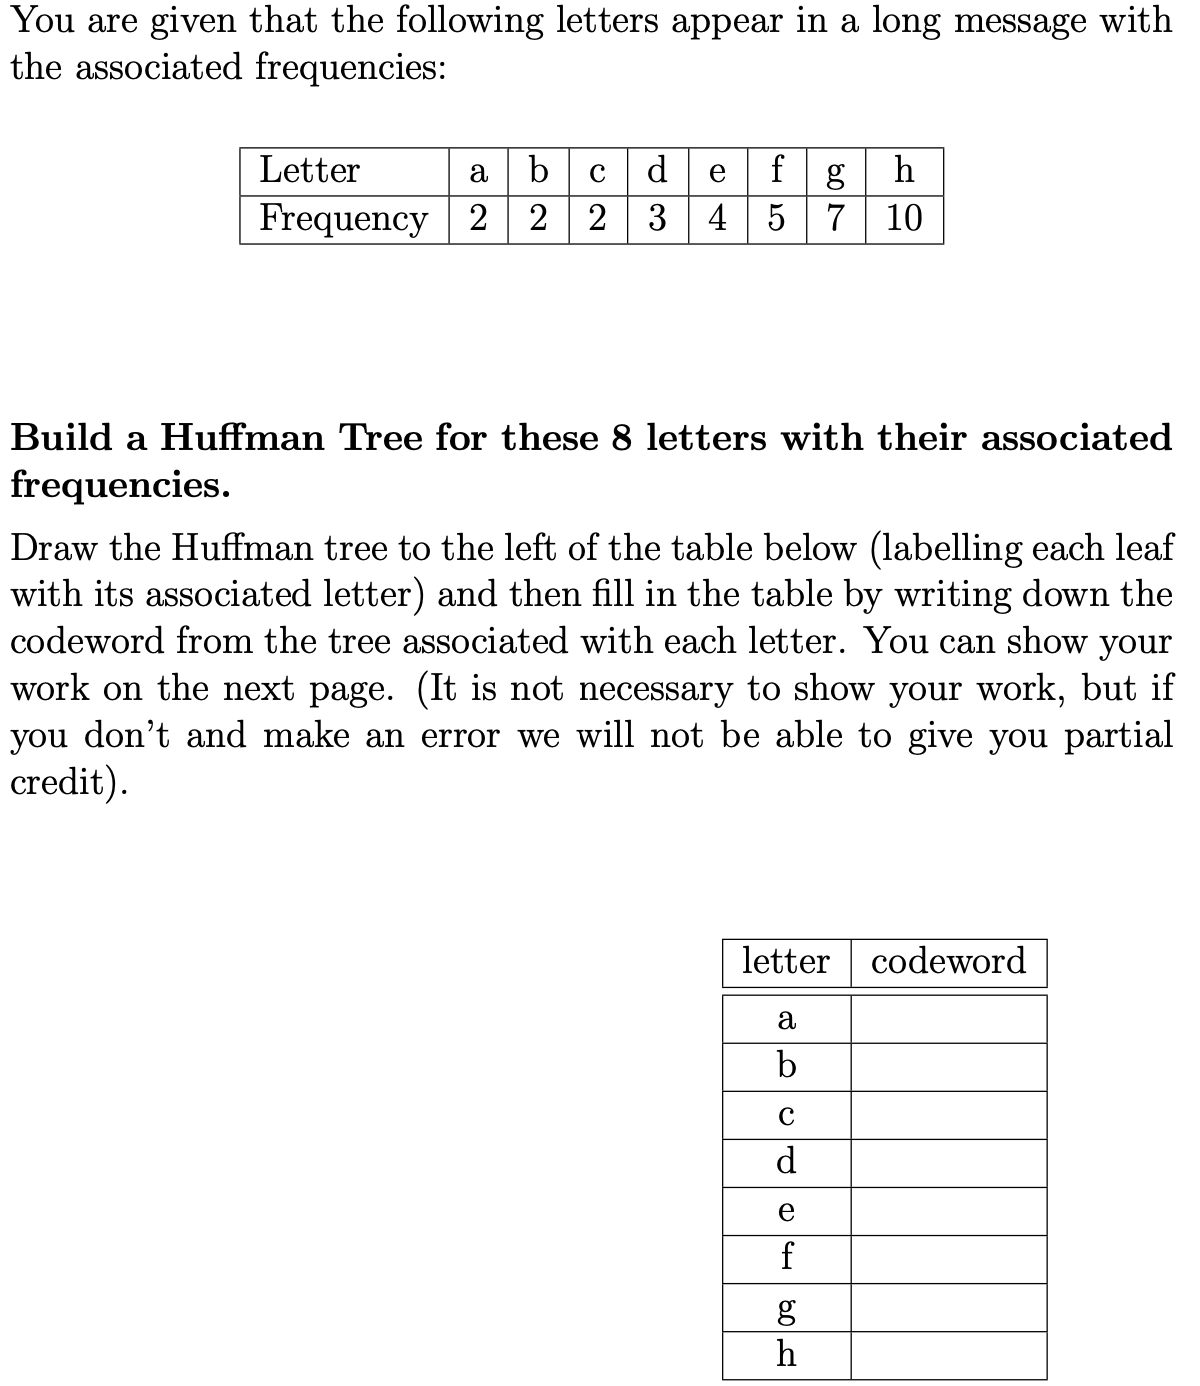
\includegraphics[scale=0.65]{images/07-exercise-2019s-huffman-question.png}

    \newpage
    5. (2021Fall, Assignment 3, Problem 4, 29pts) {\bf Greedy Covering}

    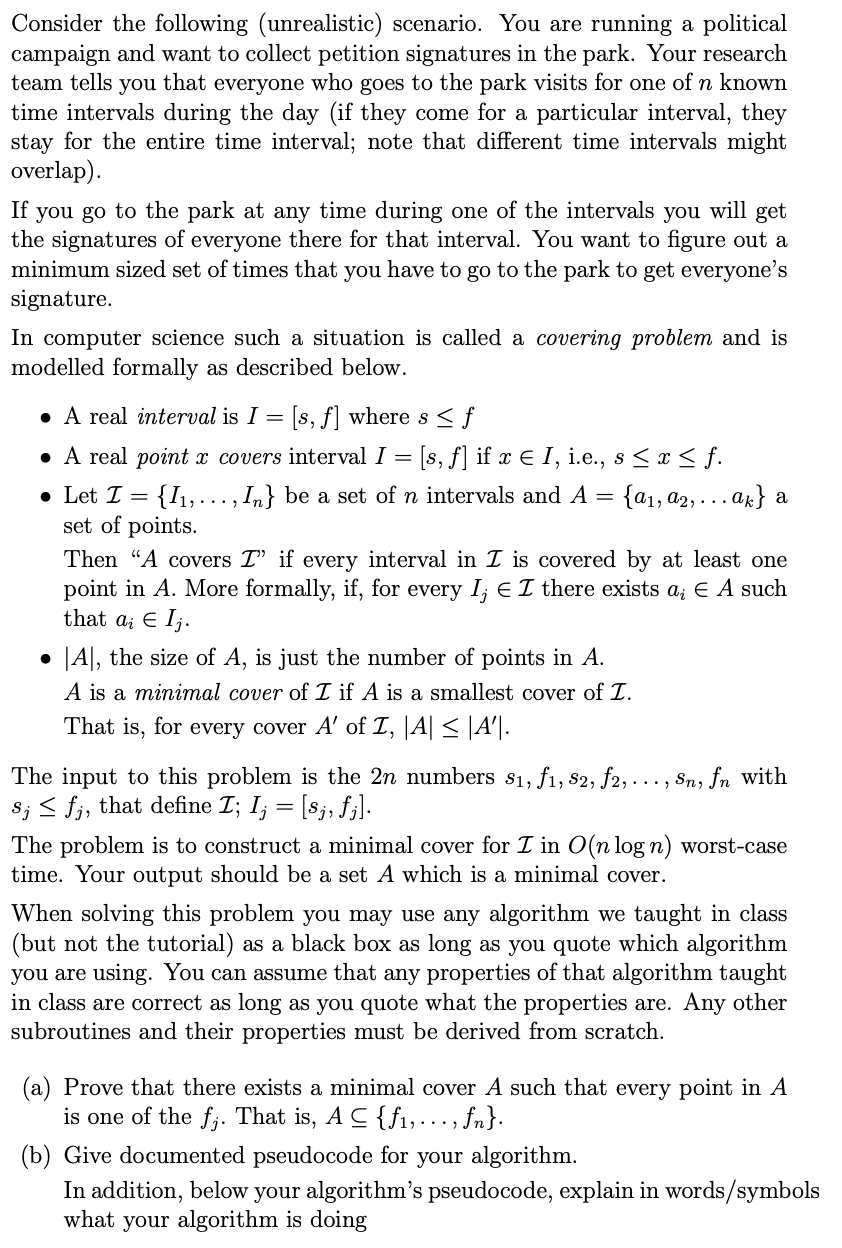
\includegraphics[scale=1.05]{images/07-exercise-2021f-hw-question.png}

    \newpage
    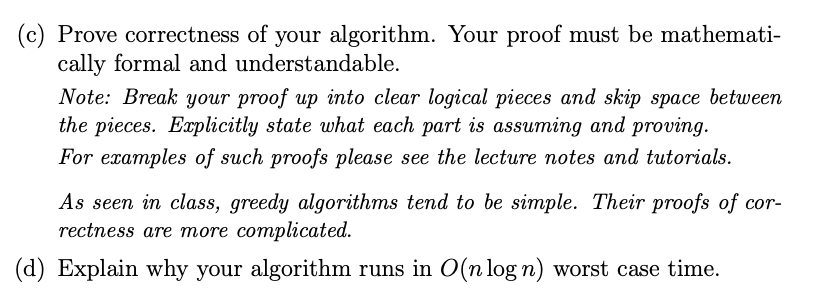
\includegraphics[scale=1.05]{images/07-exercise-2021f-hw-question2.png}



    \newpage
    \section{Solution to Exercises}

    1. (2019Spring, Midterm, 3, 18pts) {\bf Interval Scheduling} 

    (a) When the intervals are sorted by increasing start time the solution does not have to be correct. Consider this counterexample:
    $$
    I_{1}=(1,6), I_{2}=(2,3), I_{3}=(4,5).
    $$
    The optimal solution is $\left\{I_{2}, I_{3}\right\}$ while the greedy algorithm will return just the one interval $\left\{I_{1}\right\}$.
    
    (b) When the intervals are sorted by increasing finish time the solution us optimal.
    
    This is the analysis from the class notes:
    
    \setlength{\parindent}{2em}

    (a) Assume greedy is different than OPT
    
    (b) Let $i_{1}, i_{2}, \ldots, i_{k}$ denote the set of intervals selected by greedy We are ordering them so that $i_{1}<i_{2}<\cdots$
    
    (c) Let $j_{1}, j_{2}, \ldots, j_{m}$ denote the set of intervals selected by OPT Again we are ordering them so that $j_{1}<j_{2}<\cdots$
    Since an interval must end before the next one starts this means $f_{j_{r}} \leq s_{j_{r+1}}$ for all $r$
    
    (d) Note that by the definition of OPT, $m \geq k$.
    
    (e) Find largest possible value of $r$ such that $i_{1}=j_{1}, i_{2}=j_{2}, \ldots$, $i_{r}=j_{r}$.
    This means that we can write OPT as
    $$
    O P T=i_{1}, i_{2}, \ldots, i_{r}, \mathbf{j}_{\mathbf{r}+1}, j_{r+2}, \ldots, j_{m} .
    $$
    Note that it's possible that $r=0$.
    
    (f) By the definition of the greedy algorithm $j_{r+1}$ can not finish before $i_{r+1}$, otherwise the greedy algorithm would have chosen $j_{r+1}$. This means that $f_{i_{r+1}} \leq f_{j_{r+1}}$
    
    (g) From the comment in (c) above, this automatically implies that $f_{i_{r+1}} \leq f_{j_{r+1}} \leq s_{j_{r+2}}$.
    This simply means that we can replace $j_{r+1}$ with $i_{r+1}$ in OPT and still have a set of compatable coverings. This gives us
    $$
    O P T^{\prime}=i_{1}, i_{2}, \ldots, i_{r}, \mathbf{i}_{\mathbf{r}+\mathbf{1}}, j_{r+2}, \ldots, j_{m} .
    $$
    Now note that size $\left(O P T^{\prime}\right)=m=\operatorname{size}(O P T)$ so $O P T^{\prime}$ is also optimal.
    
    (h) We have therefore found an optimal solution that agrees with OPT with at least $r+1$ places instead of $r$ places.
    
    (i) We can repeat lines (a)-(g) until we have found an optimal solution OPT that agrees with greedy on all of its first $k$ places
    
    (j) If $m>k$ then greedy could have chosen $j_{k+1}$ after choosing $i_{k}$. Since greedy did not choose it, $j_{k+1}$ does not exist so $m=k$.
    
    (k) Since $m=k$, greedy is optimal

    \setlength{\parindent}{0em}

    \vspace{0.5in}
    2. (2021Spring, Final, 3, 14pts) {\bf Greedy Classroom Scheduling} 

    (a) Here is the proof we derived in class.
    \begin{itemize}
        \item (A) The depth of a set of open intervals is the maximum number of classes that exist at any instant of time.
        \item  - Let $t$ be some time at which depth classes exist simultaneously. Such a $t$ must exist from the definition of depth.
        \item  - At this time $t$, at least $d$ classrooms must be open to host the depth classes.
        \item  - $\Rightarrow$ (B) any class scheduling solution must open at least depth classrooms
        \item - Now, let $d$ be the number of classrooms opened by the greedy algorithm.
        \item - Classroom $d$ is opened because we needed to schedule a lecture, say $j$, that is incompatible with all $d-1$ other classrooms.
        \item - Since we sorted by start time, all these incompatibilities are caused by lectures that all start no later than $s_{j}$ and finish later than $s_{j}$
        \item - Thus, there is a time at which $d$ lectures all overlap. The time is $s_{j}+\epsilon$ for some $\epsilon>0$; the $d$ lectures are the $d-1$ incompatible ones and lecture $j$,
        \item - $\Rightarrow(\mathrm{C})$ depth $\geq d$
        \item - Since every schedule must use at least depth classrooms and greedy uses only $d \leq$ depth classrooms, greedy uses no more than any other solution so greedy is optimal.
    \end{itemize}

    (b) We can keep the classrooms in a min-heap (min priority queue) using the finishing times of the last class in the room as the classroom's key.
    
    To check in line 4 whether there is a compatible classroom we do an extract$\min$ to find the minimum finishing time currently stored in the priority queue.
    
    If line 5 is called, then just insert the new finishing time $s_{j}$ to p.queue
    
    If line 8 is called, then re-insert that minimum finishing time back into the p.queue AND insert the new finishing time $s_{j}$ into the p.queue
    
    Note that extract-mins and inserts can be performed in $O(\log N)$ time in a min priority queue with $N$ items. Since the number of items in the queue at any specific time will be $O(n)$, each extract-min and insert operation will $\operatorname{cost} O(\log n)$ time; thus, each call to line $(*),(* *)$ or $(* * *)$ will require only $O(\log n)$ time.
    
    Since each of lines $4,5,7$ are called at most once for each value of $j$, the total work for performing them is $O(n \log n)$ time. The sort in line (1) also requires $O(n \log n)$ time so the entire algorithm uses only $O(n \log n)$ time.


    \vspace{0.5in}
    3. (2020Spring, Final, 1, 15pts) {\bf Greedy Algorithms} 

    {\it The solution to this problem is so long, please refer to past paper.}

    \vspace{0.5in}
    4. (2019Spring, Midterm, 2, 10pts) {\bf Huffman Coding}

    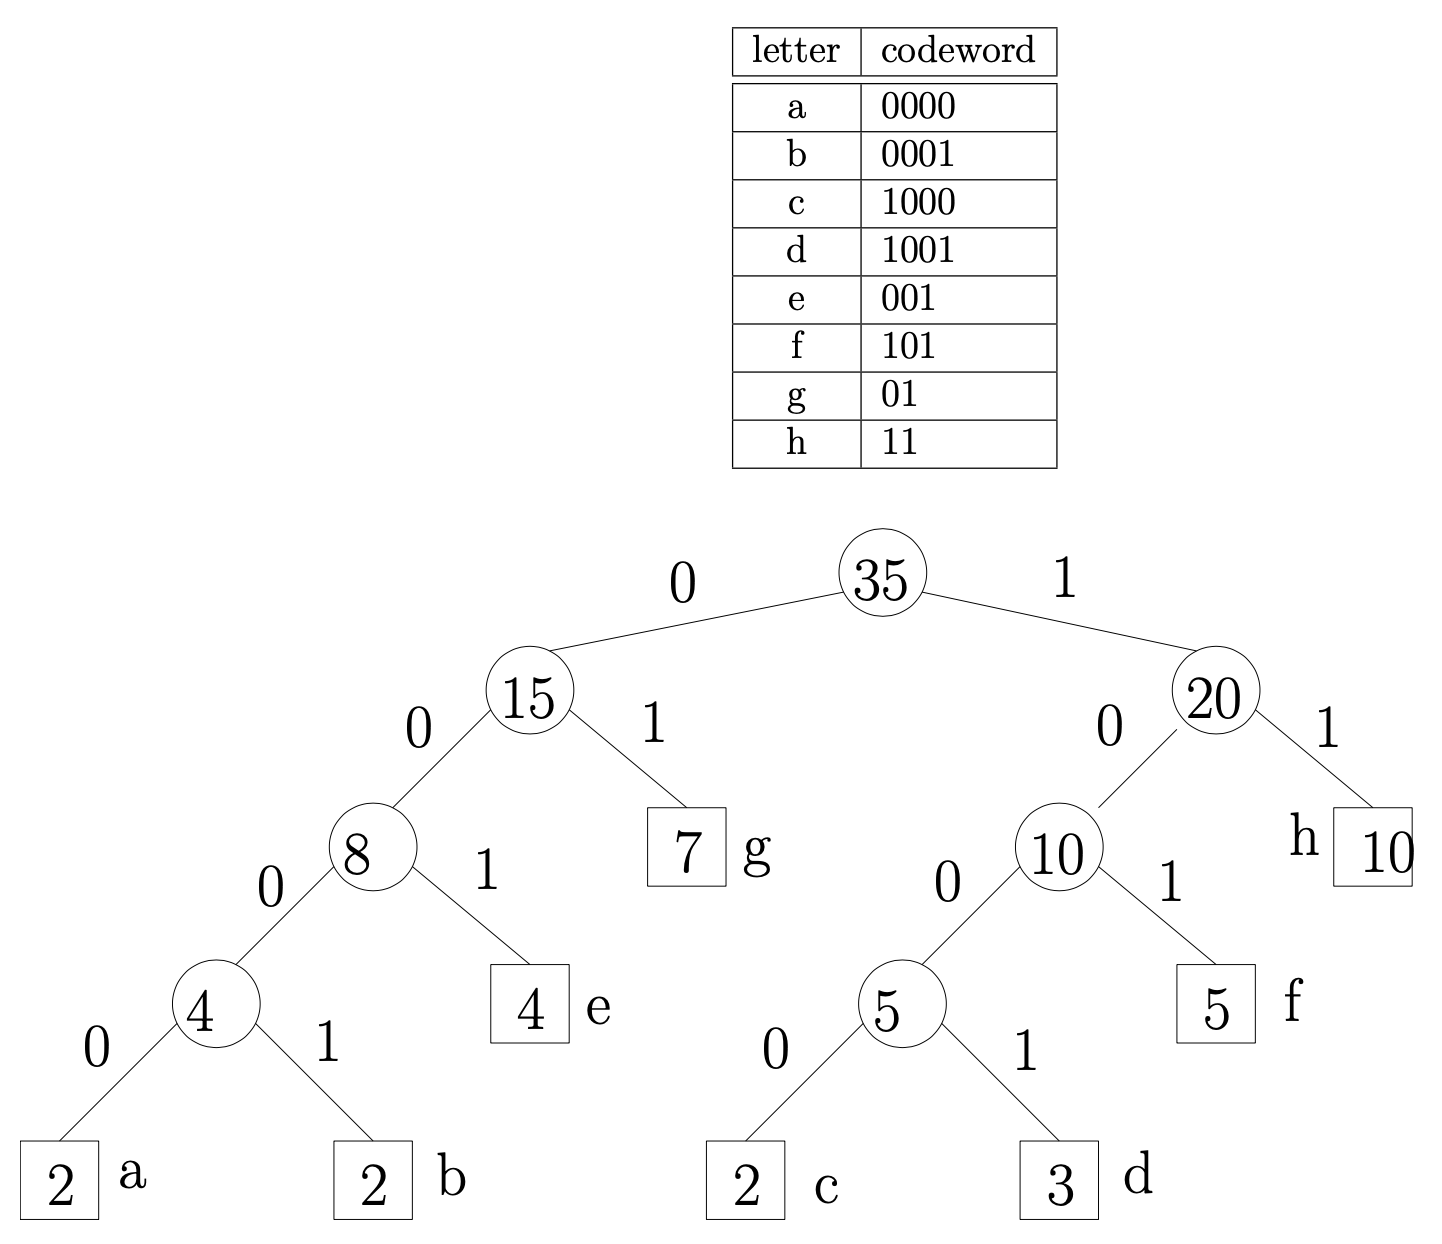
\includegraphics[scale=0.55]{images/07-exercise-2019s-huffman-sol.png}

    \newpage
    5. (2021Fall, Assignment 3, Problem 4, 29pts) {\bf Greedy Covering} 

    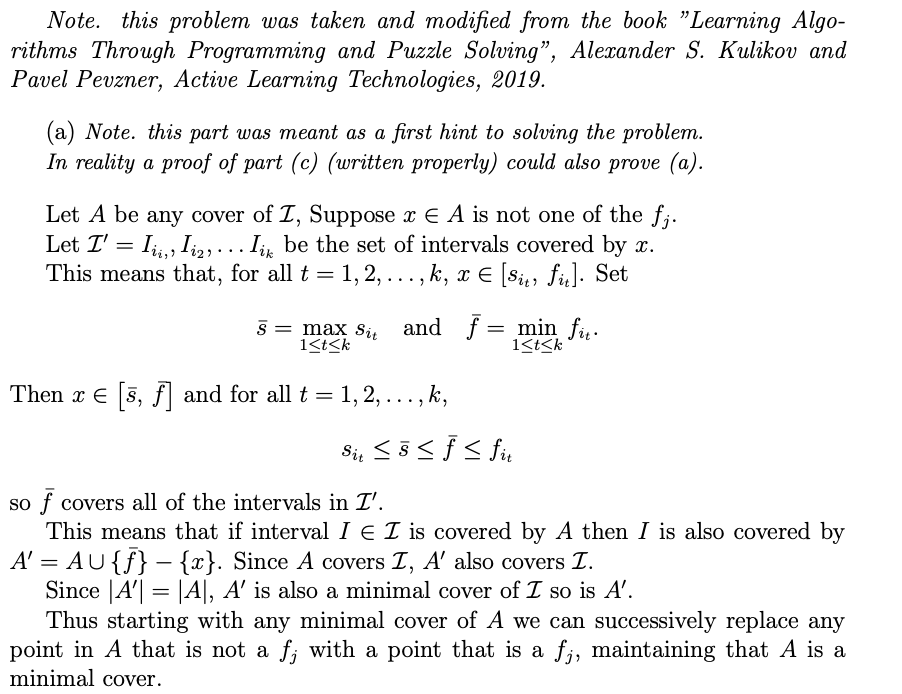
\includegraphics[scale=1.05]{images/07-exercise-2021f-hw-sol1}

    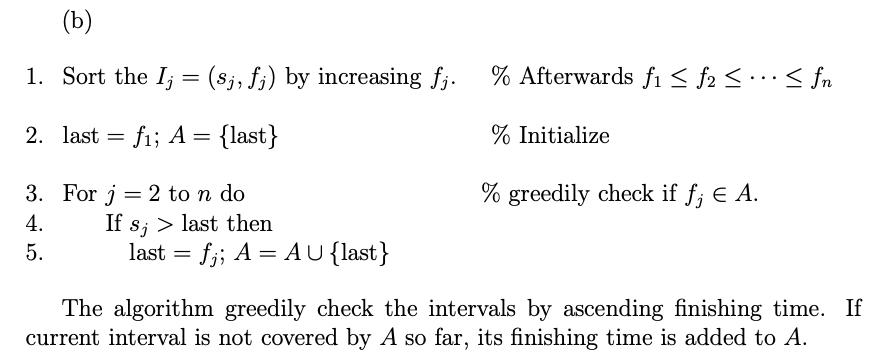
\includegraphics[scale=1.05]{images/07-exercise-2021f-hw-sol2}

    \newpage
    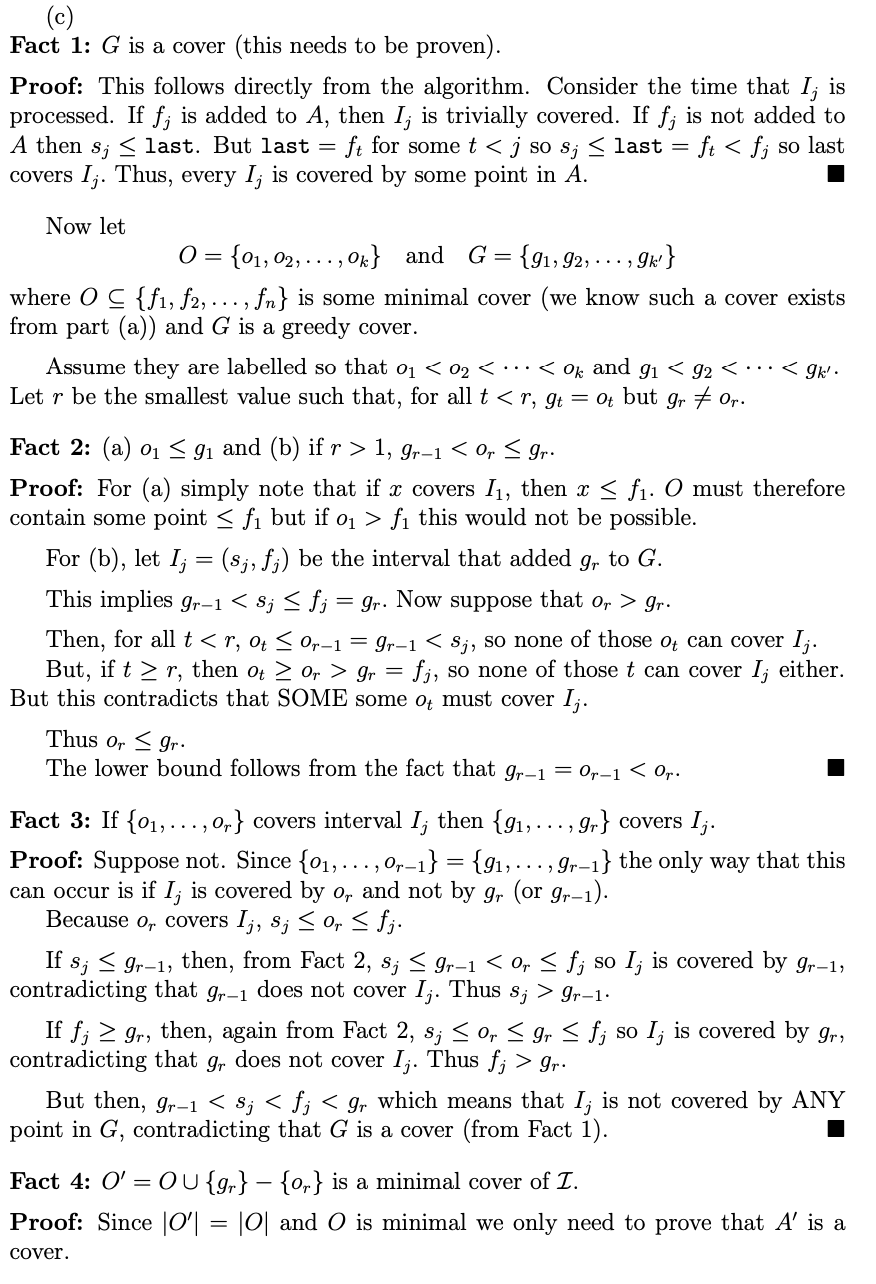
\includegraphics[scale=1.05]{images/07-exercise-2021f-hw-sol3}

    \newpage
    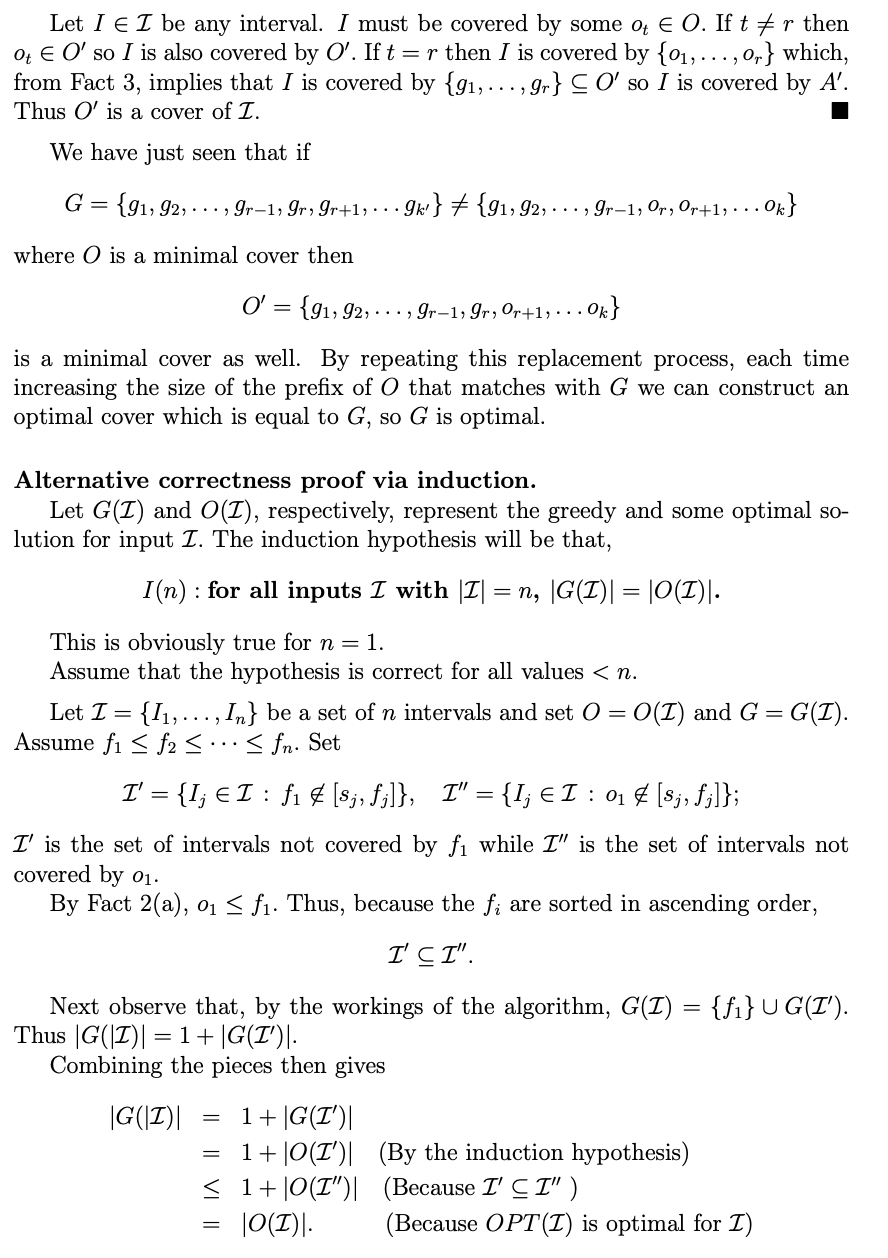
\includegraphics[scale=1.05]{images/07-exercise-2021f-hw-sol4}

    \newpage
    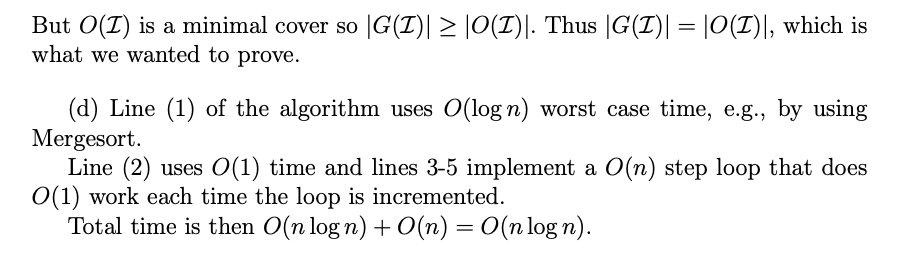
\includegraphics[scale=1.00]{images/07-exercise-2021f-hw-sol5}

\end{spacing}

\chapter{Dynamic Programming: 1D}

\input{Chapters/Ch08-DP.tex}

\chapter{Dynamic Programming: 2D}

\chapter{Dynamic Programming: over intervals}




% %----------------------------------------------------------------------------------------
% %	CHAPTER 1
% %----------------------------------------------------------------------------------------

% \chapterimage{chapter_head_2.pdf} % Chapter heading image

% \chapter{Asymptotic}

% \section{Paragraphs of Text}\index{Paragraphs of Text}

% \lipsum[1-7] % Dummy text

% %------------------------------------------------

% \section{Citation}\index{Citation}

% This statement requires citation \cite{article_key}; this one is more specific \cite[162]{book_key}.

% %------------------------------------------------

% \section{Lists}\index{Lists}

% Lists are useful to present information in a concise and/or ordered way\footnote{Footnote example...}.

% \subsection{Numbered List}\index{Lists!Numbered List}

% \begin{enumerate}
% \item The first item
% \item The second item
% \item The third item
% \end{enumerate}

% \subsection{Bullet Points}\index{Lists!Bullet Points}

% \begin{itemize}
% \item The first item
% \item The second item
% \item The third item
% \end{itemize}

% \subsection{Descriptions and Definitions}\index{Lists!Descriptions and Definitions}

% \begin{description}
% \item[Name] Description
% \item[Word] Definition
% \item[Comment] Elaboration
% \end{description}

% %----------------------------------------------------------------------------------------
% %	CHAPTER 2
% %----------------------------------------------------------------------------------------

% \chapter{In-text Elements}

% \section{Theorems}\index{Theorems}

% This is an example of theorems.

% \subsection{Several equations}\index{Theorems!Several Equations}
% This is a theorem consisting of several equations.

% \begin{theorem}[Name of the theorem]
% In $E=\mathbb{R}^n$ all norms are equivalent. It has the properties:
% \begin{align}
% & \big| ||\mathbf{x}|| - ||\mathbf{y}|| \big|\leq || \mathbf{x}- \mathbf{y}||\\
% &  ||\sum_{i=1}^n\mathbf{x}_i||\leq \sum_{i=1}^n||\mathbf{x}_i||\quad\text{where $n$ is a finite integer}
% \end{align}
% \end{theorem}

% \subsection{Single Line}\index{Theorems!Single Line}
% This is a theorem consisting of just one line.

% \begin{theorem}
% A set $\mathcal{D}(G)$ in dense in $L^2(G)$, $|\cdot|_0$. 
% \end{theorem}

% %------------------------------------------------

% \section{Definitions}\index{Definitions}

% This is an example of a definition. A definition could be mathematical or it could define a concept.

% \begin{definition}[Definition name]
% Given a vector space $E$, a norm on $E$ is an application, denoted $||\cdot||$, $E$ in $\mathbb{R}^+=[0,+\infty[$ such that:
% \begin{align}
% & ||\mathbf{x}||=0\ \Rightarrow\ \mathbf{x}=\mathbf{0}\\
% & ||\lambda \mathbf{x}||=|\lambda|\cdot ||\mathbf{x}||\\
% & ||\mathbf{x}+\mathbf{y}||\leq ||\mathbf{x}||+||\mathbf{y}||
% \end{align}
% \end{definition}

% %------------------------------------------------

% \section{Notations}\index{Notations}

% \begin{notation}
% Given an open subset $G$ of $\mathbb{R}^n$, the set of functions $\varphi$ are:
% \begin{enumerate}
% \item Bounded support $G$;
% \item Infinitely differentiable;
% \end{enumerate}
% a vector space is denoted by $\mathcal{D}(G)$. 
% \end{notation}

% %------------------------------------------------

% \section{Remarks}\index{Remarks}

% This is an example of a remark.

% \begin{remark}
% The concepts presented here are now in conventional employment in mathematics. Vector spaces are taken over the field $\mathbb{K}=\mathbb{R}$, however, established properties are easily extended to $\mathbb{K}=\mathbb{C}$.
% \end{remark}

% %------------------------------------------------

% \section{Corollaries}\index{Corollaries}

% This is an example of a corollary.

% \begin{corollary}[Corollary name]
% The concepts presented here are now in conventional employment in mathematics. Vector spaces are taken over the field $\mathbb{K}=\mathbb{R}$, however, established properties are easily extended to $\mathbb{K}=\mathbb{C}$.
% \end{corollary}

% %------------------------------------------------

% \section{Propositions}\index{Propositions}

% This is an example of propositions.

% \subsection{Several equations}\index{Propositions!Several Equations}

% \begin{proposition}[Proposition name]
% It has the properties:
% \begin{align}
% & \big| ||\mathbf{x}|| - ||\mathbf{y}|| \big|\leq || \mathbf{x}- \mathbf{y}||\\
% &  ||\sum_{i=1}^n\mathbf{x}_i||\leq \sum_{i=1}^n||\mathbf{x}_i||\quad\text{where $n$ is a finite integer}
% \end{align}
% \end{proposition}

% \subsection{Single Line}\index{Propositions!Single Line}

% \begin{proposition} 
% Let $f,g\in L^2(G)$; if $\forall \varphi\in\mathcal{D}(G)$, $(f,\varphi)_0=(g,\varphi)_0$ then $f = g$. 
% \end{proposition}

% %------------------------------------------------

% \section{Examples}\index{Examples}

% This is an example of examples.

% \subsection{Equation and Text}\index{Examples!Equation and Text}

% \begin{example}
% Let $G=\{x\in\mathbb{R}^2:|x|<3\}$ and denoted by: $x^0=(1,1)$; consider the function:
% \begin{equation}
% f(x)=\left\{\begin{aligned} & \mathrm{e}^{|x|} & & \text{si $|x-x^0|\leq 1/2$}\\
% & 0 & & \text{si $|x-x^0|> 1/2$}\end{aligned}\right.
% \end{equation}
% The function $f$ has bounded support, we can take $A=\{x\in\mathbb{R}^2:|x-x^0|\leq 1/2+\epsilon\}$ for all $\epsilon\in\intoo{0}{5/2-\sqrt{2}}$.
% \end{example}

% \subsection{Paragraph of Text}\index{Examples!Paragraph of Text}

% \begin{example}[Example name]
% \lipsum[2]
% \end{example}

% %------------------------------------------------

% \section{Exercises}\index{Exercises}

% This is an example of an exercise.

% \begin{exercise}
% This is a good place to ask a question to test learning progress or further cement ideas into students' minds.
% \end{exercise}

% %------------------------------------------------

% \section{Problems}\index{Problems}

% \begin{problem}
% What is the average airspeed velocity of an unladen swallow?
% \end{problem}

% %------------------------------------------------

% \section{Vocabulary}\index{Vocabulary}

% Define a word to improve a students' vocabulary.

% \begin{vocabulary}[Word]
% Definition of word.
% \end{vocabulary}

% %----------------------------------------------------------------------------------------
% %	PART
% %----------------------------------------------------------------------------------------

% \part{Part Two}

% %----------------------------------------------------------------------------------------
% %	CHAPTER 3
% %----------------------------------------------------------------------------------------

% \chapterimage{chapter_head_1.pdf} % Chapter heading image

% \chapter{Presenting Information}

% \section{Table}\index{Table}

% \begin{table}[h]
% \centering
% \begin{tabular}{l l l}
% \toprule
% \textbf{Treatments} & \textbf{Response 1} & \textbf{Response 2}\\
% \midrule
% Treatment 1 & 0.0003262 & 0.562 \\
% Treatment 2 & 0.0015681 & 0.910 \\
% Treatment 3 & 0.0009271 & 0.296 \\
% \bottomrule
% \end{tabular}
% \caption{Table caption}
% \label{tab:example} % Unique label used for referencing the table in-text
% %\addcontentsline{toc}{table}{Table \ref{tab:example}} % Uncomment to add the table to the table of contents
% \end{table}

% Referencing Table \ref{tab:example} in-text automatically.

% %------------------------------------------------

% \section{Figure}\index{Figure}

% \begin{figure}[h]
% \centering
\includegraphics[scale=0.5]{placeholder.jpg}
% \caption{Figure caption}
% \label{fig:placeholder} % Unique label used for referencing the figure in-text
% %\addcontentsline{toc}{figure}{Figure \ref{fig:placeholder}} % Uncomment to add the figure to the table of contents
% \end{figure}

% Referencing Figure \ref{fig:placeholder} in-text automatically.

% %----------------------------------------------------------------------------------------
% %	BIBLIOGRAPHY
% %----------------------------------------------------------------------------------------

% \chapter*{Bibliography}
% \addcontentsline{toc}{chapter}{\textcolor{ocre}{Bibliography}} % Add a Bibliography heading to the table of contents

% %------------------------------------------------

% \section*{Articles}
% \addcontentsline{toc}{section}{Articles}
% \printbibliography[heading=bibempty,type=article]

% %------------------------------------------------

% \section*{Books}
% \addcontentsline{toc}{section}{Books}
% \printbibliography[heading=bibempty,type=book]

% %----------------------------------------------------------------------------------------
% %	INDEX
% %----------------------------------------------------------------------------------------

% \cleardoublepage % Make sure the index starts on an odd (right side) page
% \phantomsection
% \setlength{\columnsep}{0.75cm} % Space between the 2 columns of the index
% \addcontentsline{toc}{chapter}{\textcolor{ocre}{Index}} % Add an Index heading to the table of contents
% \printindex % Output the index

% %----------------------------------------------------------------------------------------

\end{document}
